\documentclass{article}
% generated by Madoko, version 1.1.4
%mdk-data-line={1}


\usepackage[heading-base={2},section-num={False},bib-label={hide},fontspec={True}]{madoko2}


\begin{document}



%mdk-data-line={15}
\noindent\mdline{15}IC-FEDS WEBSITE SCREENS%mdk

%mdk-data-line={61}
\section{\mdline{61}1.\hspace*{0.5em}\mdline{61}SCREENS SECTION}\label{sec-screens-section}%mdk%mdk

%mdk-data-line={64}
\noindent\mdline{64}This section shows the screens that were designed
corresponding to the various Insurance Commission processes that were
selected for Proof-of-Concept development. Note that the website will
have screens for Insurance Commission examiners, and screens for the
users from regulated entities (companies). This document presents both
types of screens together, organized by IC Division, for greater ease of
understanding.%mdk

%mdk-data-line={74}
\mdline{74}The screens presented here are updated from the preliminary
designs that are included in the System Design Specification
document.The updates are based on the comments of IC staff who reviewed
the site during user-acceptance testing. A compilation of these comments
can be found in the Comments Section of this document.%mdk

%mdk-data-line={80}
\section{\mdline{80}2.\hspace*{0.5em}\mdline{80}FINANCIAL EXAMINATIONS GROUP}\label{sec-financial-examinations-group}%mdk%mdk

%mdk-data-line={83}
\subsection{\mdline{83}2.1.\hspace*{0.5em}\mdline{83}1.  Brokers Division}\label{sec-1-brokers-division}%mdk%mdk

%mdk-data-line={86}
\noindent\mdline{86}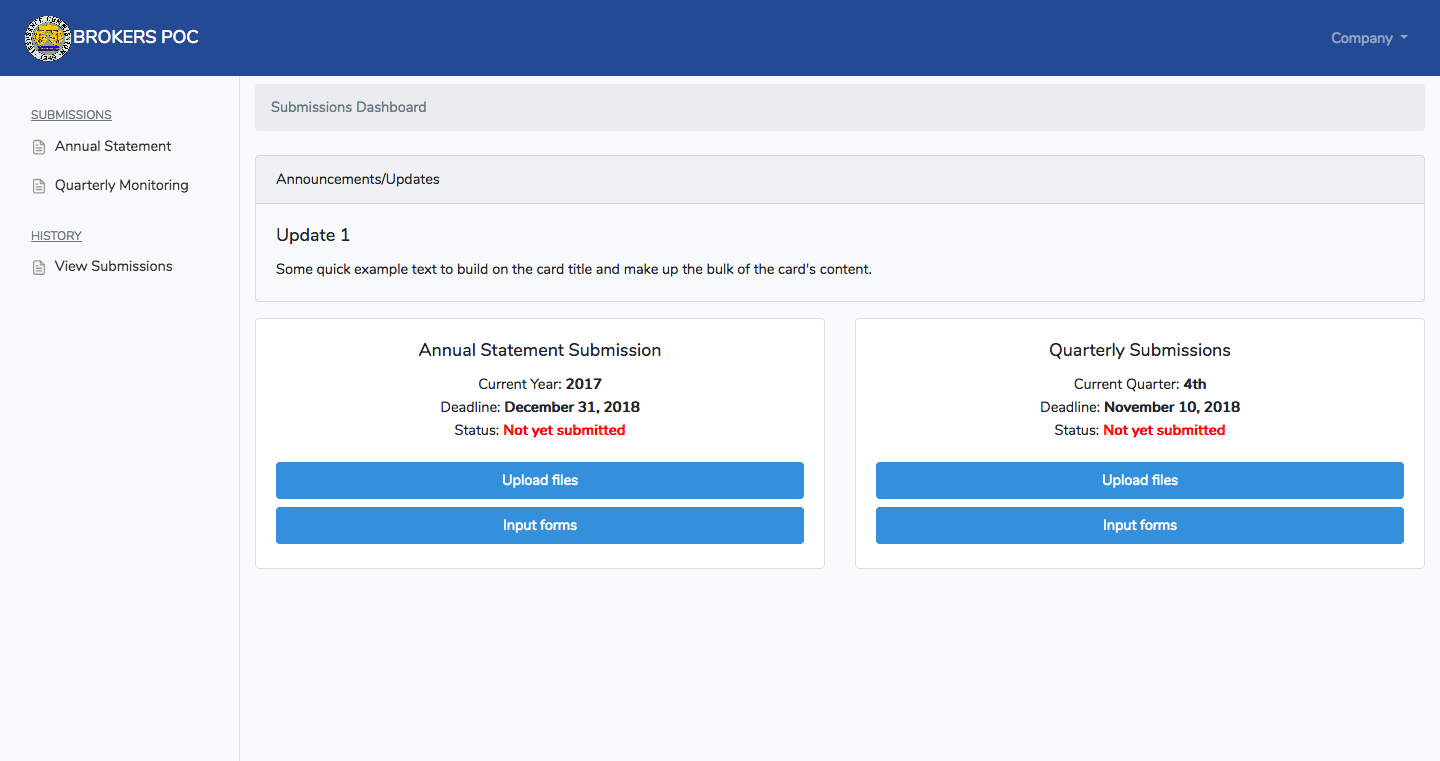
\includegraphics[keepaspectratio=true]{up-ic-screens/image141}{}\mdline{86}{}[\mdline{86}Company’s view\mdline{86}]\mdline{86} This is the Submissions Dashboard for
companies under Brokers Division.%mdk

%mdk-data-line={89}
\mdline{89}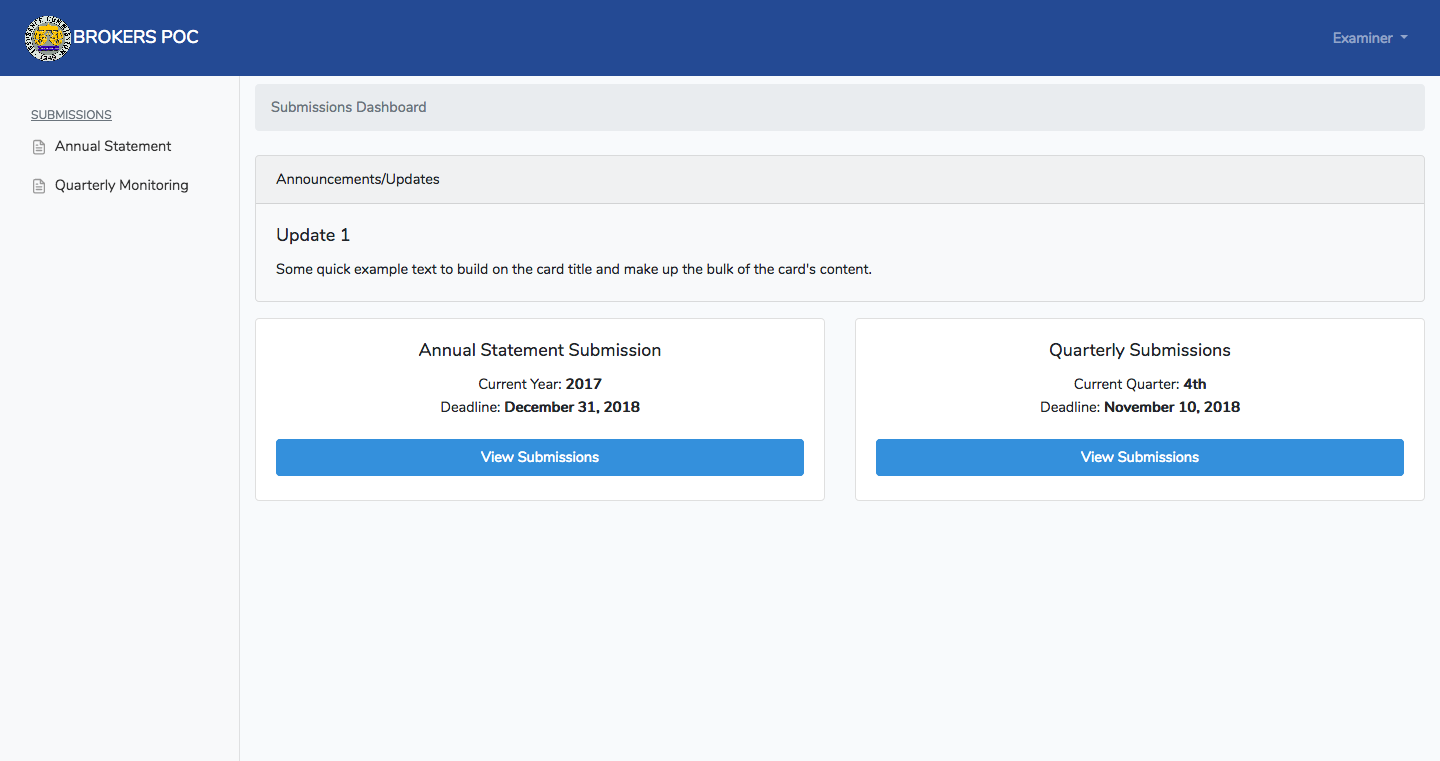
\includegraphics[keepaspectratio=true]{up-ic-screens/image92}{}\mdline{89}{}[\mdline{89}Examiner’s view\mdline{89}]\mdline{89} This is the dashboard for examiners of
 Brokers Division.%mdk

%mdk-data-line={96}
\begin{enumerate}[noitemsep,topsep=\mdcompacttopsep]%mdk

%mdk-data-line={96}
\item{}
%mdk-data-line={96}
\subsubsection{\mdline{96}2.1.1.\hspace*{0.5em}\mdline{96}Annual Submission and Examination of Financial Condition/Standing}\label{sec-annual-submission-and-examination-of-financial-conditionstanding}%mdk%mdk%mdk
%mdk
\end{enumerate}%mdk

%mdk-data-line={98}
\noindent\mdline{98}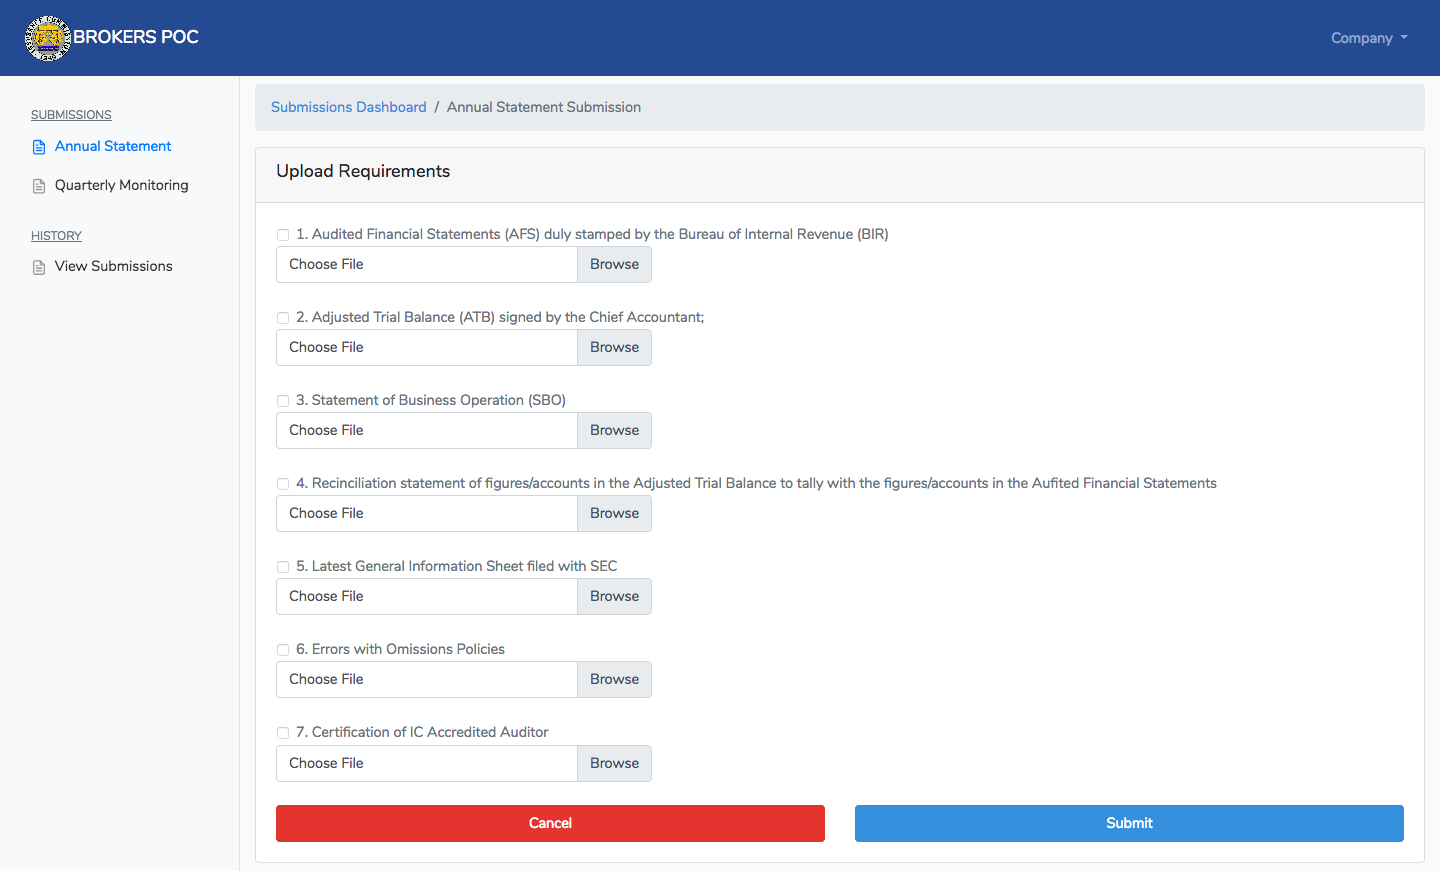
\includegraphics[keepaspectratio=true]{up-ic-screens/image108}{}\mdline{98}%mdk

%mdk-data-line={100}
\mdline{100}{}[\mdline{100}Company’s view\mdline{100}]\mdline{100} This is the screen where the company
must upload the checklist of files needed.%mdk

%mdk-data-line={103}
\mdline{103}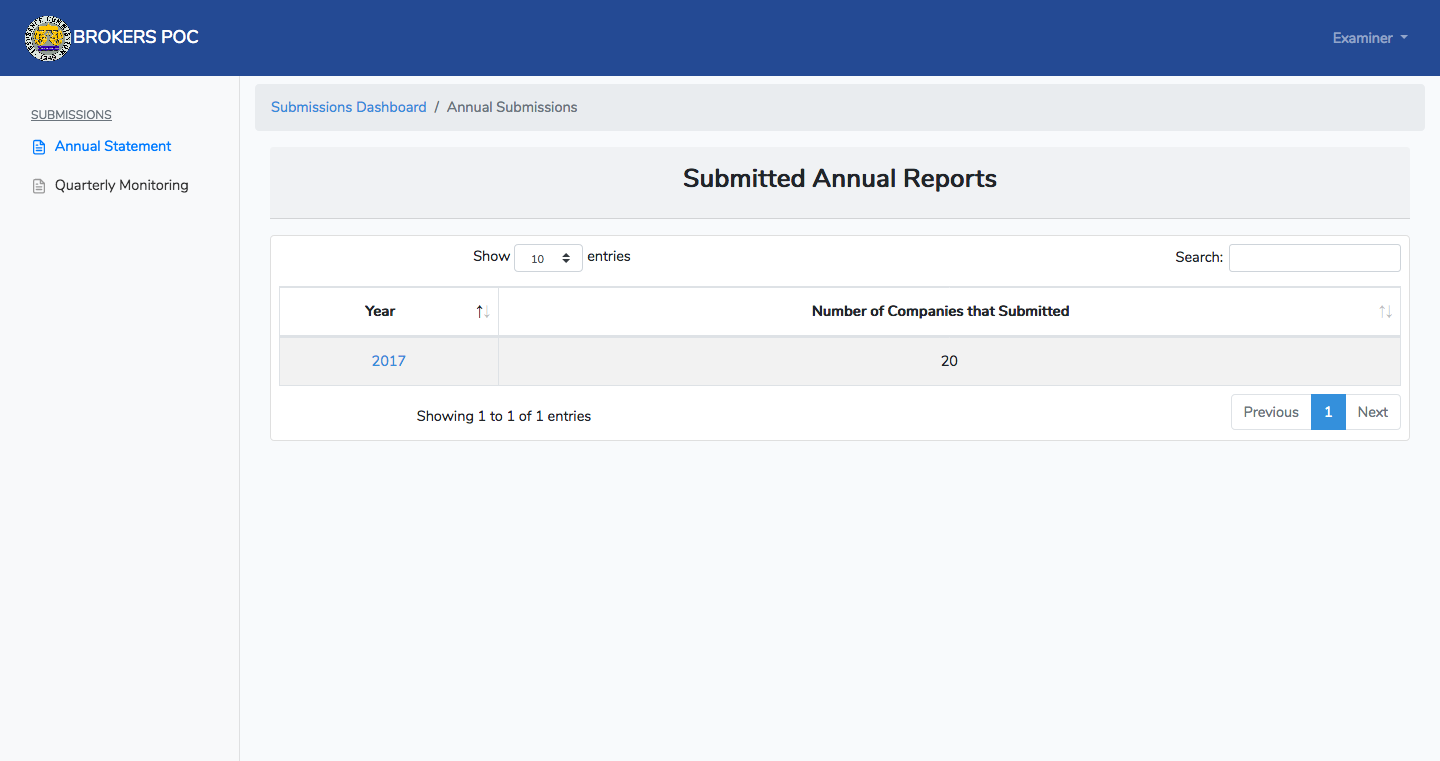
\includegraphics[keepaspectratio=true]{up-ic-screens/image138}{}\mdline{103}%mdk

%mdk-data-line={105}
\mdline{105}{}[\mdline{105}Examiner’s view\mdline{105}]\mdline{105} This is the Submitted Annual
Reports page. The year, together with the number of companies that
submitted an Annual Report,  are listed on this screen. Upon clicking
the year, the user will see the list of companies that submitted that
year.%mdk

%mdk-data-line={115}
\mdline{115}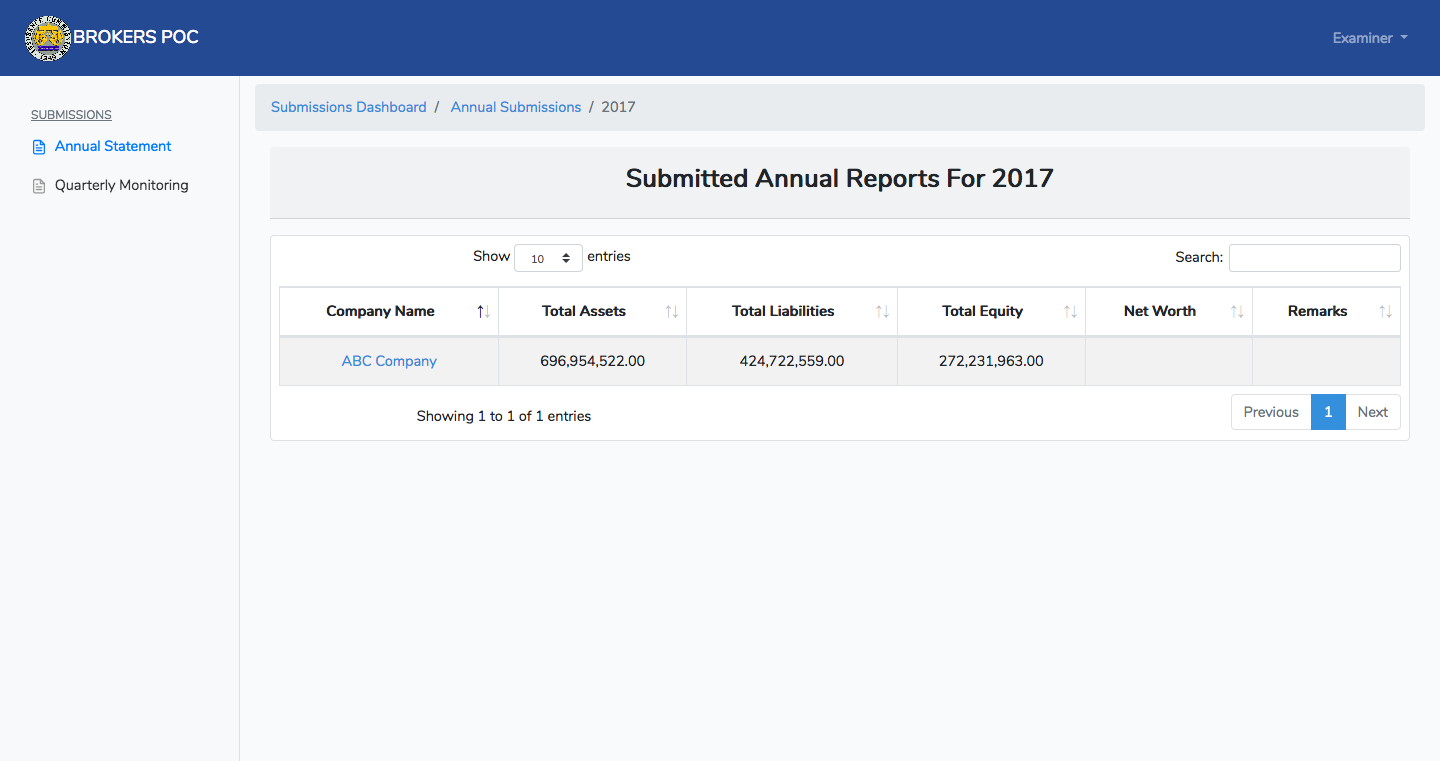
\includegraphics[keepaspectratio=true]{up-ic-screens/image76}{}\mdline{115}%mdk

%mdk-data-line={117}
\mdline{117}{}[\mdline{117}Examiner’s view\mdline{117}]\mdline{117} This is the list of companies that
submitted Annual Report for the year 2017. The name of Company, Total
Assets, Total Liabilities, Total Equity, Net Worth and Remarks are
already flashed on the screen. When the user click the company name, the
user will see the Working Balance sheet of the company.%mdk

%mdk-data-line={125}
\mdline{125}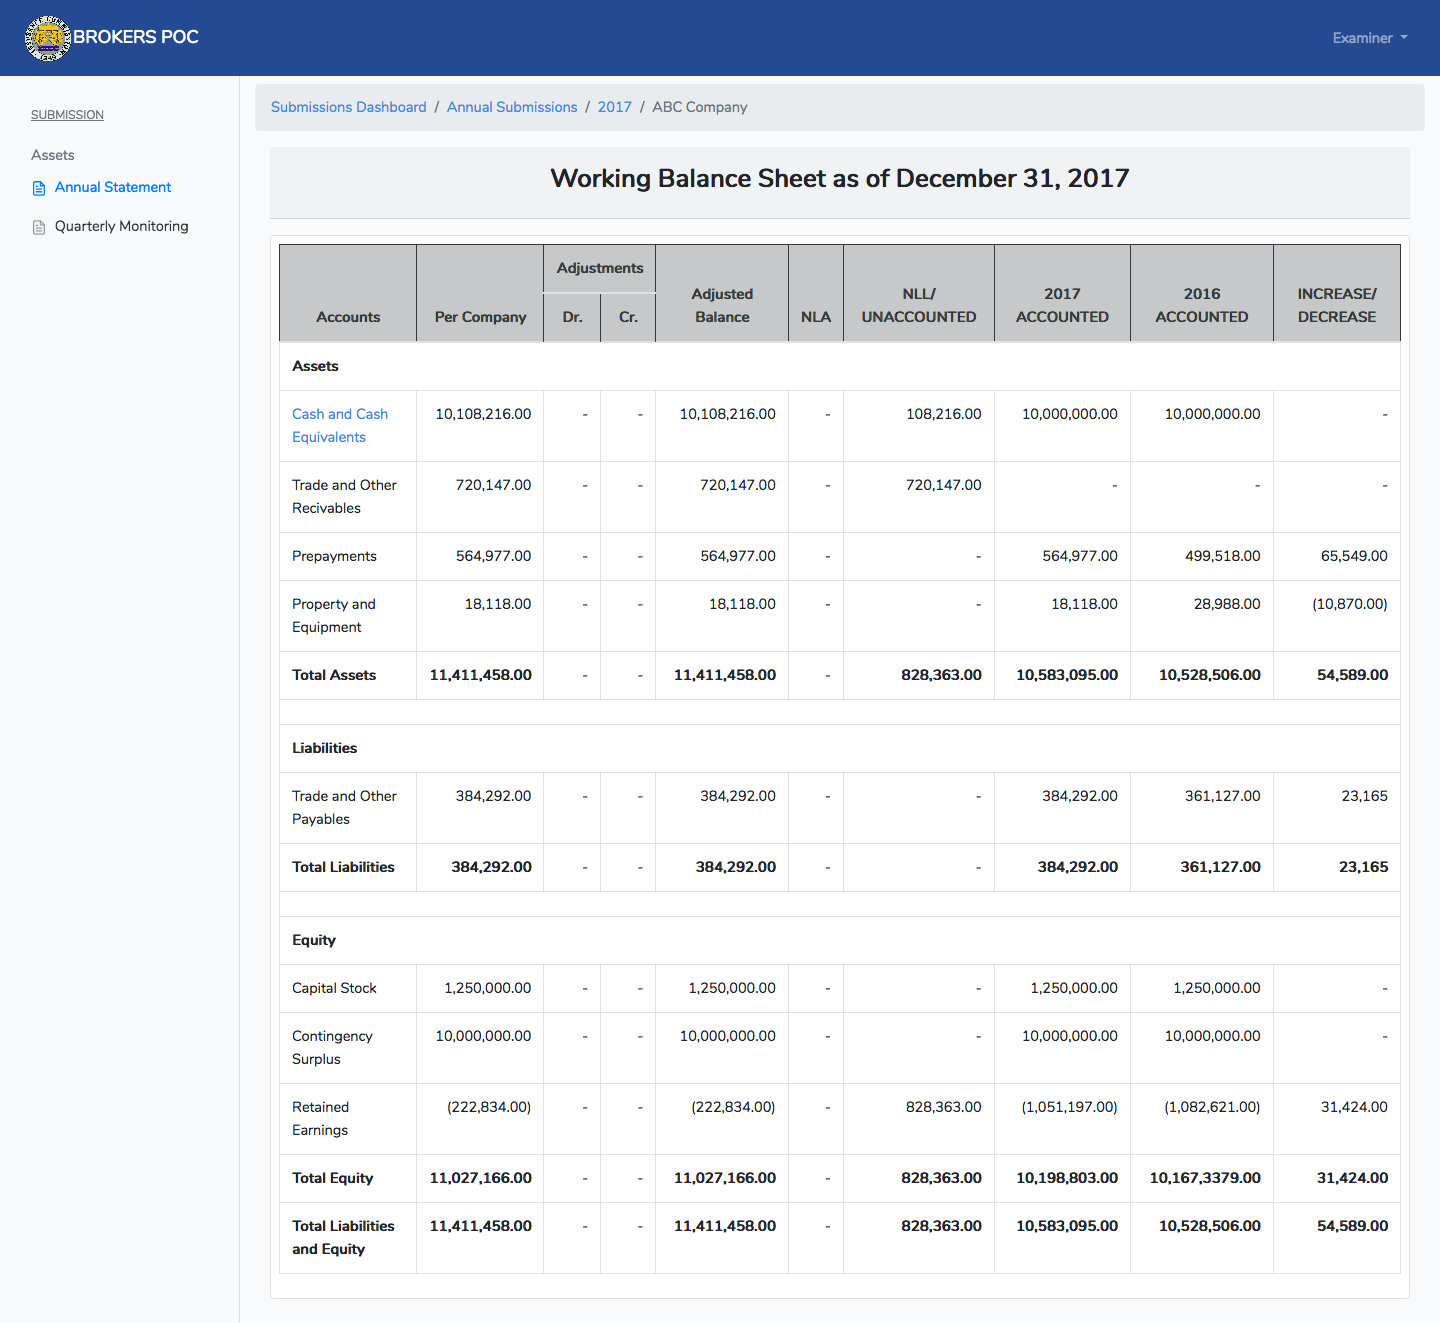
\includegraphics[keepaspectratio=true]{up-ic-screens/image35}{}\mdline{125}{}[\mdline{125}Examiner’s view\mdline{125}]\mdline{125} This is the Working balance sheet. When
the user click the accounts (summaries), the details will be
shown.%mdk

%mdk-data-line={131}
\mdline{131}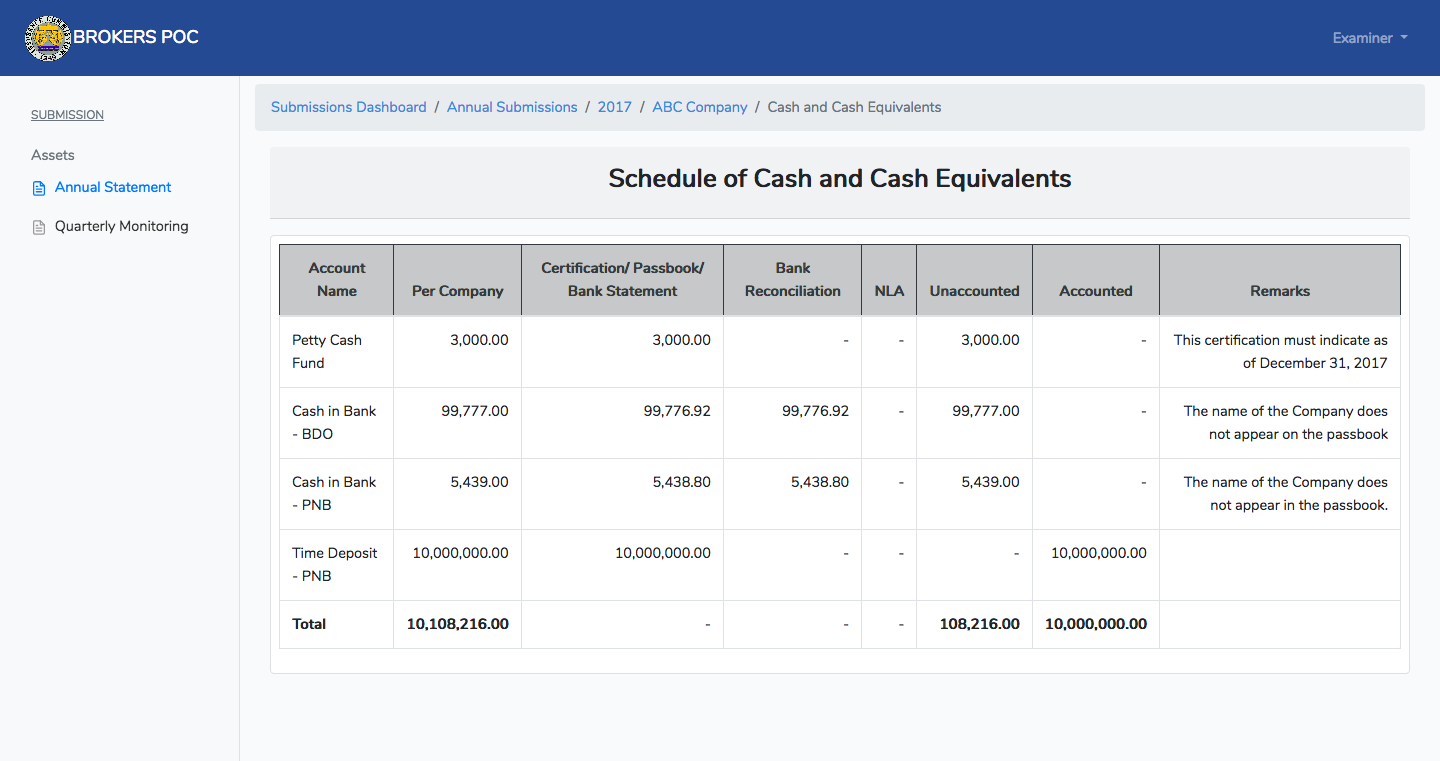
\includegraphics[keepaspectratio=true]{up-ic-screens/image135}{}\mdline{131}{}[\mdline{131}Examiner’s view\mdline{131}]\mdline{131} This is the details of the summary. For
this example, this is the Schedule of Cash and Cash Equivalents.%mdk

%mdk-data-line={138}
\begin{enumerate}[noitemsep,topsep=\mdcompacttopsep]%mdk

%mdk-data-line={138}
\item{}
%mdk-data-line={138}
\subsubsection{\mdline{138}2.1.2.\hspace*{0.5em}\mdline{138}Quarterly Submission and Monitoring of Client’s Money Compliance}\label{sec-quarterly-submission-and-monitoring-of-clients-money-compliance}%mdk%mdk%mdk
%mdk
\end{enumerate}%mdk

%mdk-data-line={140}
\noindent\mdline{140}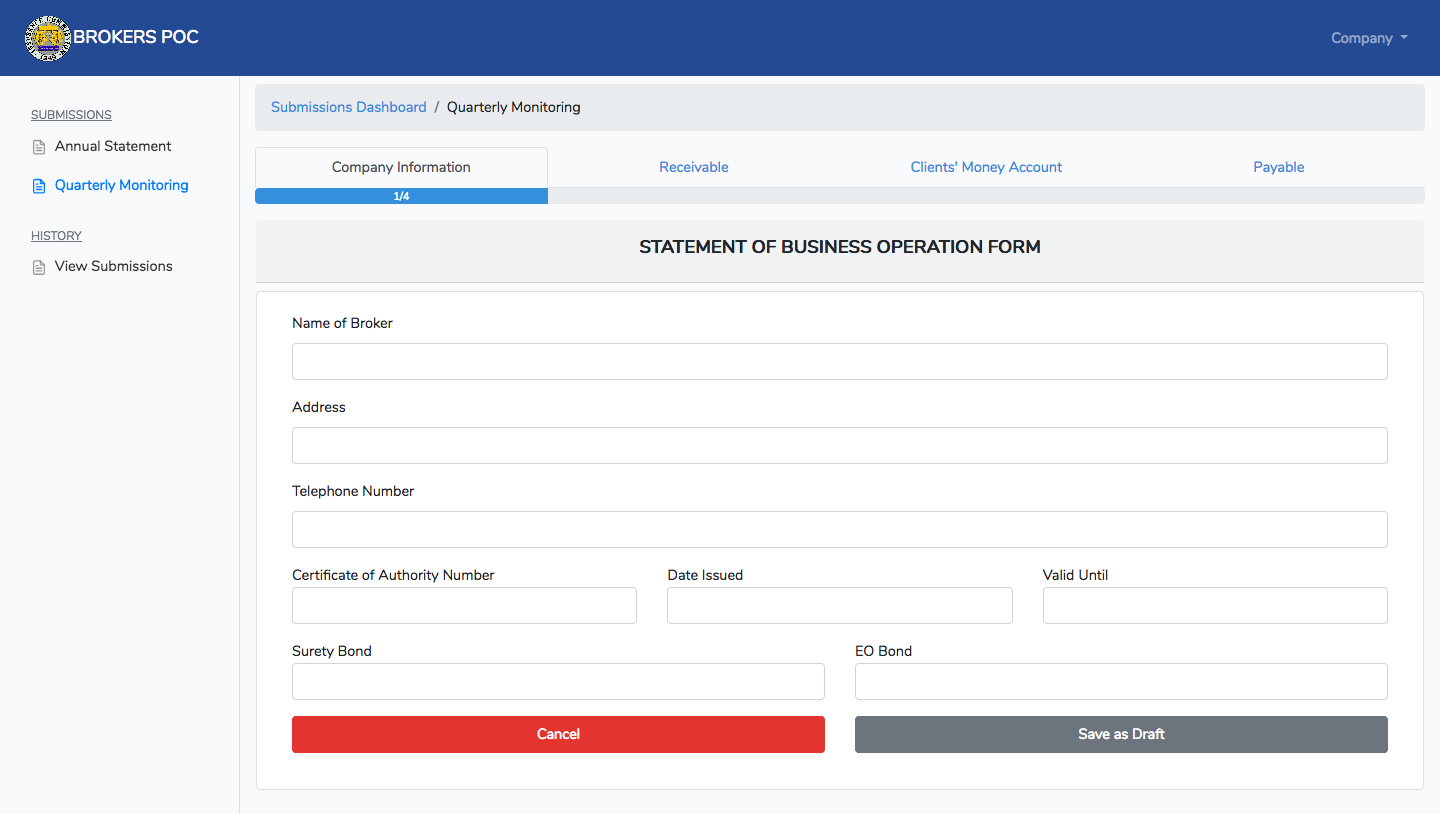
\includegraphics[keepaspectratio=true]{up-ic-screens/image55}{}\mdline{140}%mdk

%mdk-data-line={142}
\mdline{142}{}[\mdline{142}Company’s view\mdline{142}]\mdline{142} The first screen for the Statement
of Business Operation (SBO) Form is the Company Profile which will come
straight from the Licensing’s records. All forms for this process is
separated using tabs. Once the user click a tab, he/she will be
redirected to the form indicated at the top of the tab.%mdk

%mdk-data-line={150}
\mdline{150}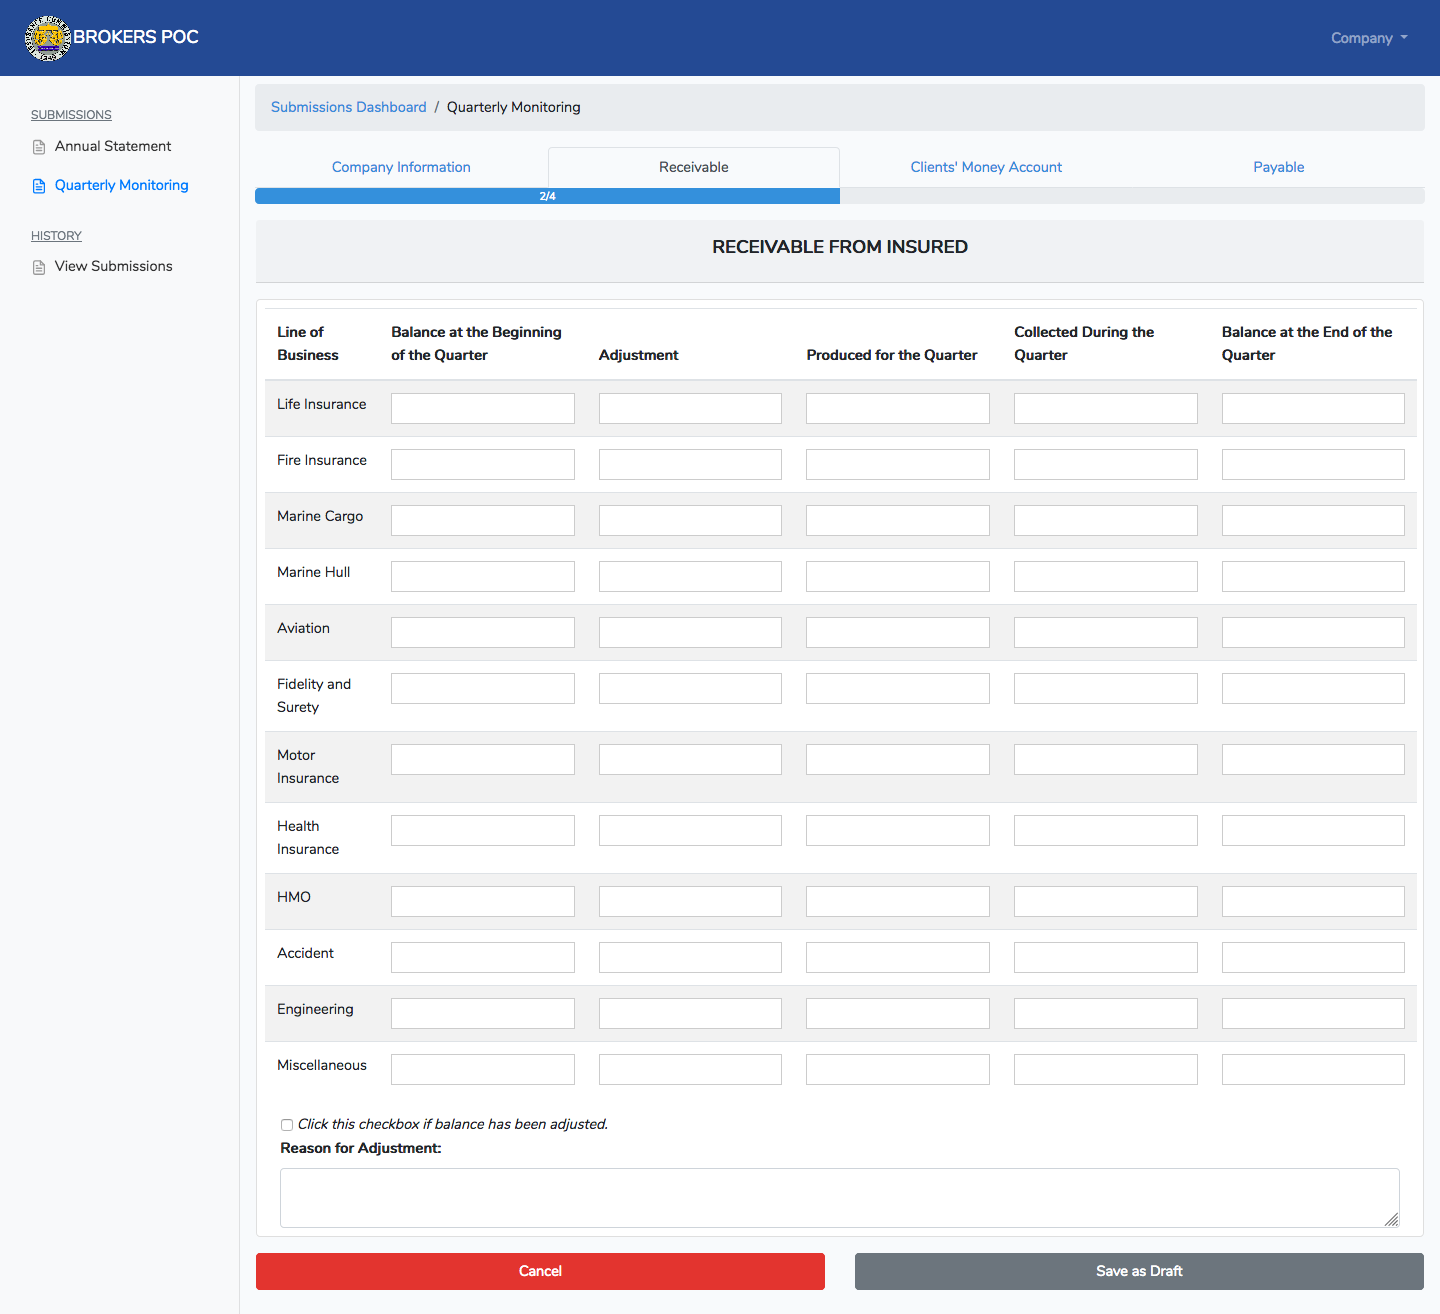
\includegraphics[keepaspectratio=true]{up-ic-screens/image160}{}\mdline{150}%mdk

%mdk-data-line={152}
\mdline{152}{}[\mdline{152}Company’s view\mdline{152}]\mdline{152} This is the Receivable from insured
tab.%mdk

%mdk-data-line={155}
\mdline{155}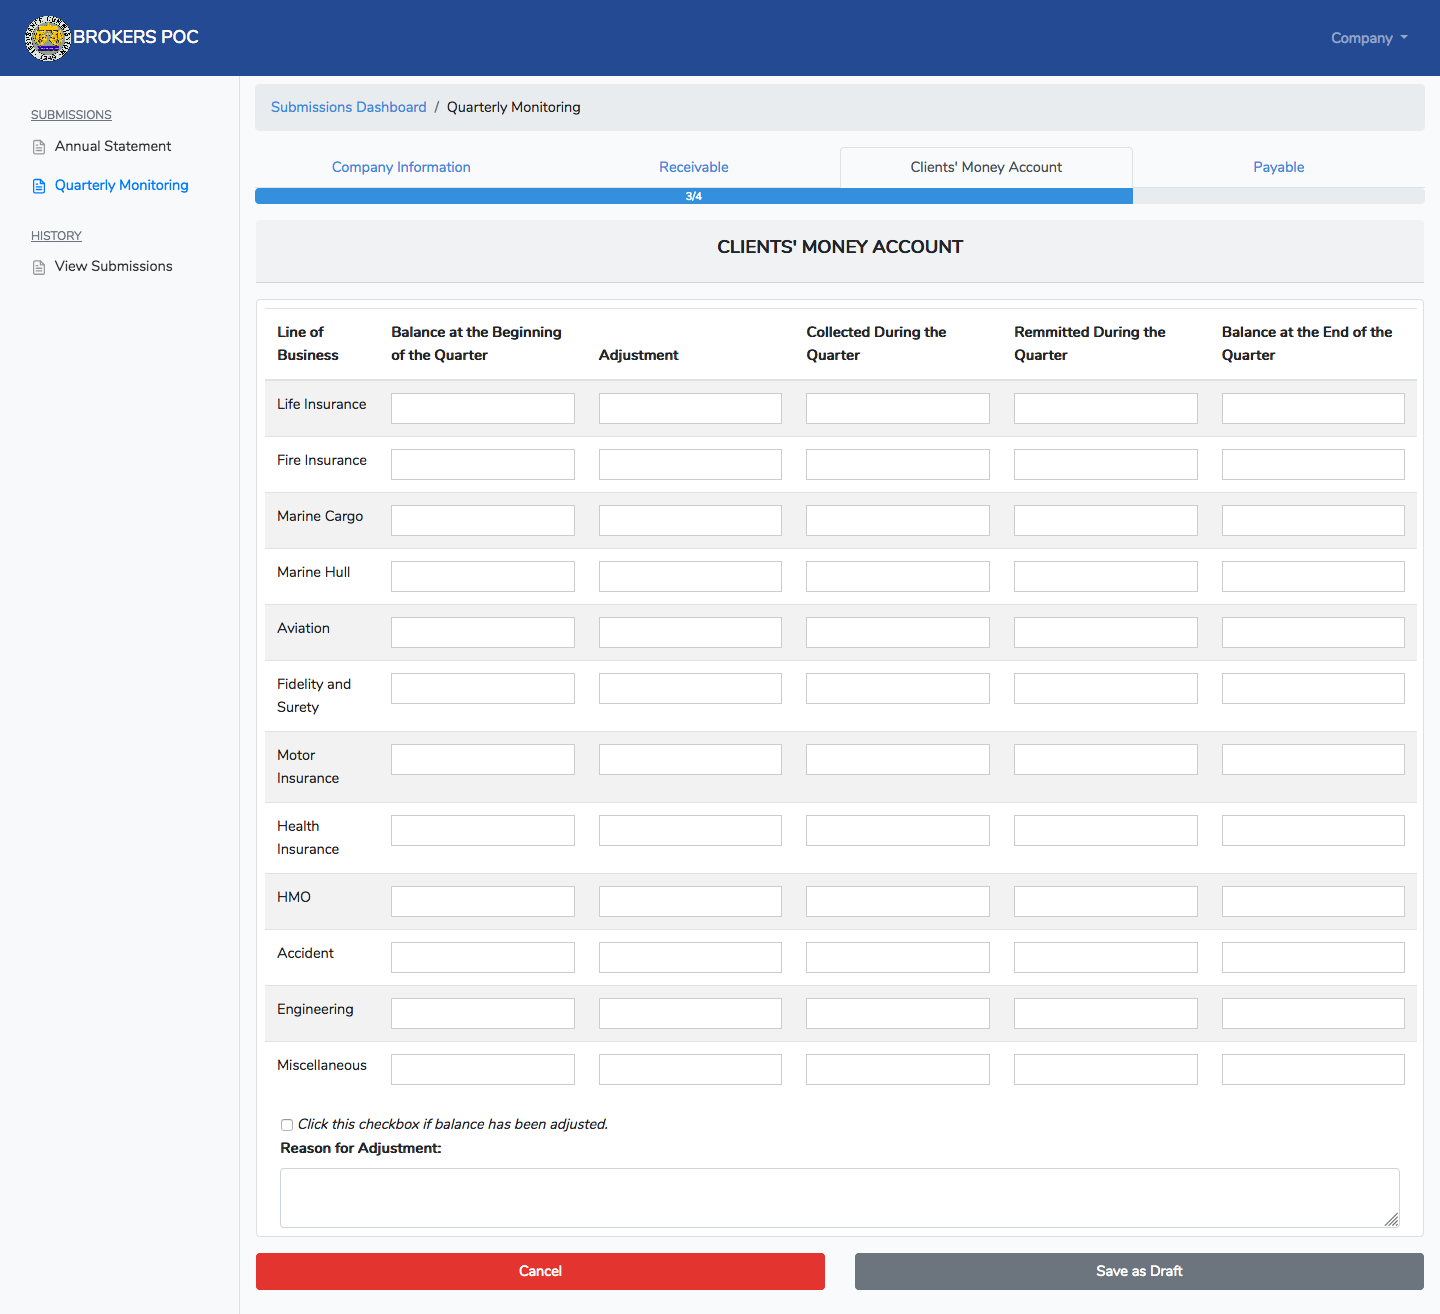
\includegraphics[keepaspectratio=true]{up-ic-screens/image180}{}\mdline{155}%mdk

%mdk-data-line={157}
\mdline{157}{}[\mdline{157}Company’s view\mdline{157}]\mdline{157} This is the Clients’ Money Account
tab.%mdk

%mdk-data-line={160}
\mdline{160}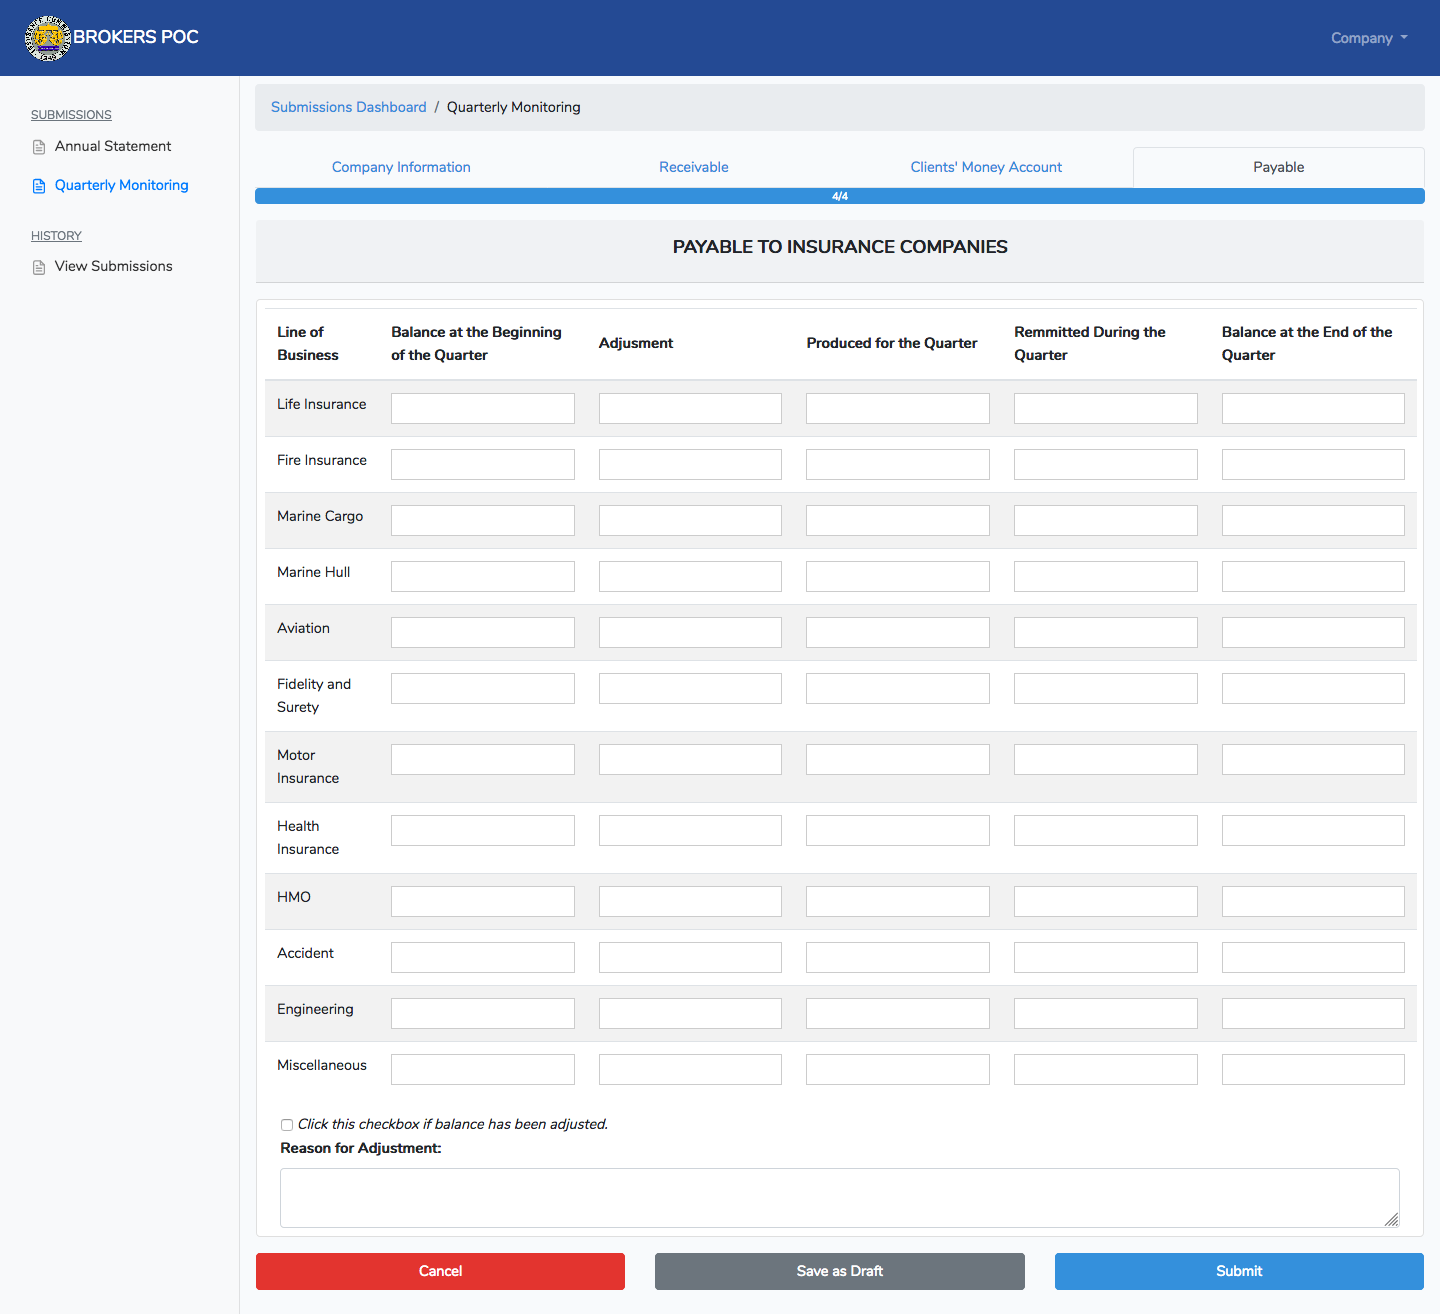
\includegraphics[keepaspectratio=true]{up-ic-screens/image149}{}\mdline{160}%mdk

%mdk-data-line={162}
\mdline{162}{}[\mdline{162}Company’s view\mdline{162}]\mdline{162} This is the Payable from Insurance
Companies tab.%mdk

%mdk-data-line={167}
\mdline{167}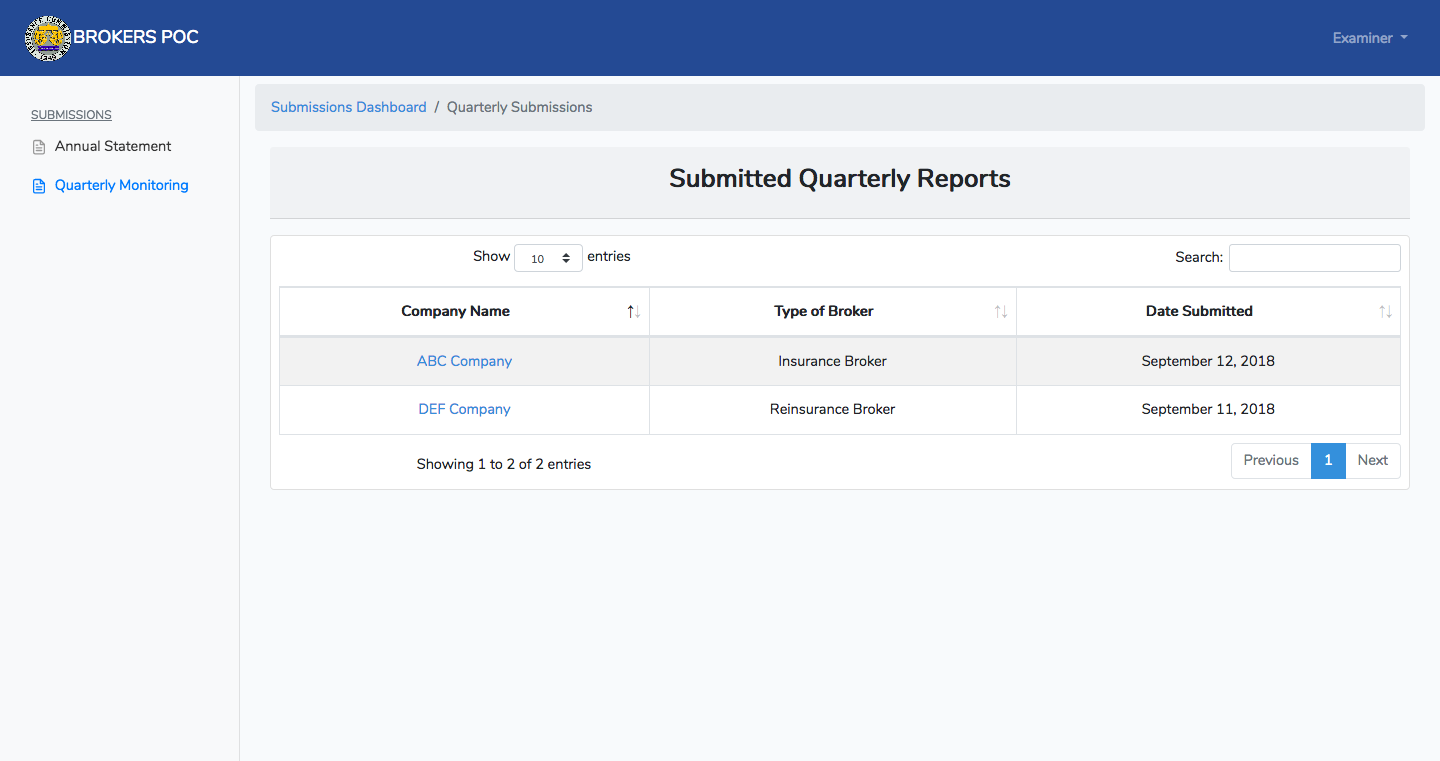
\includegraphics[keepaspectratio=true]{up-ic-screens/image74}{}\mdline{167}{}[\mdline{167}Examiner’s view\mdline{167}]\mdline{167} This screen lists all the companies that
submitted SBO. Once the examiner click the name of the company, the
screen will show the submission details of the company.%mdk

%mdk-data-line={173}
\mdline{173}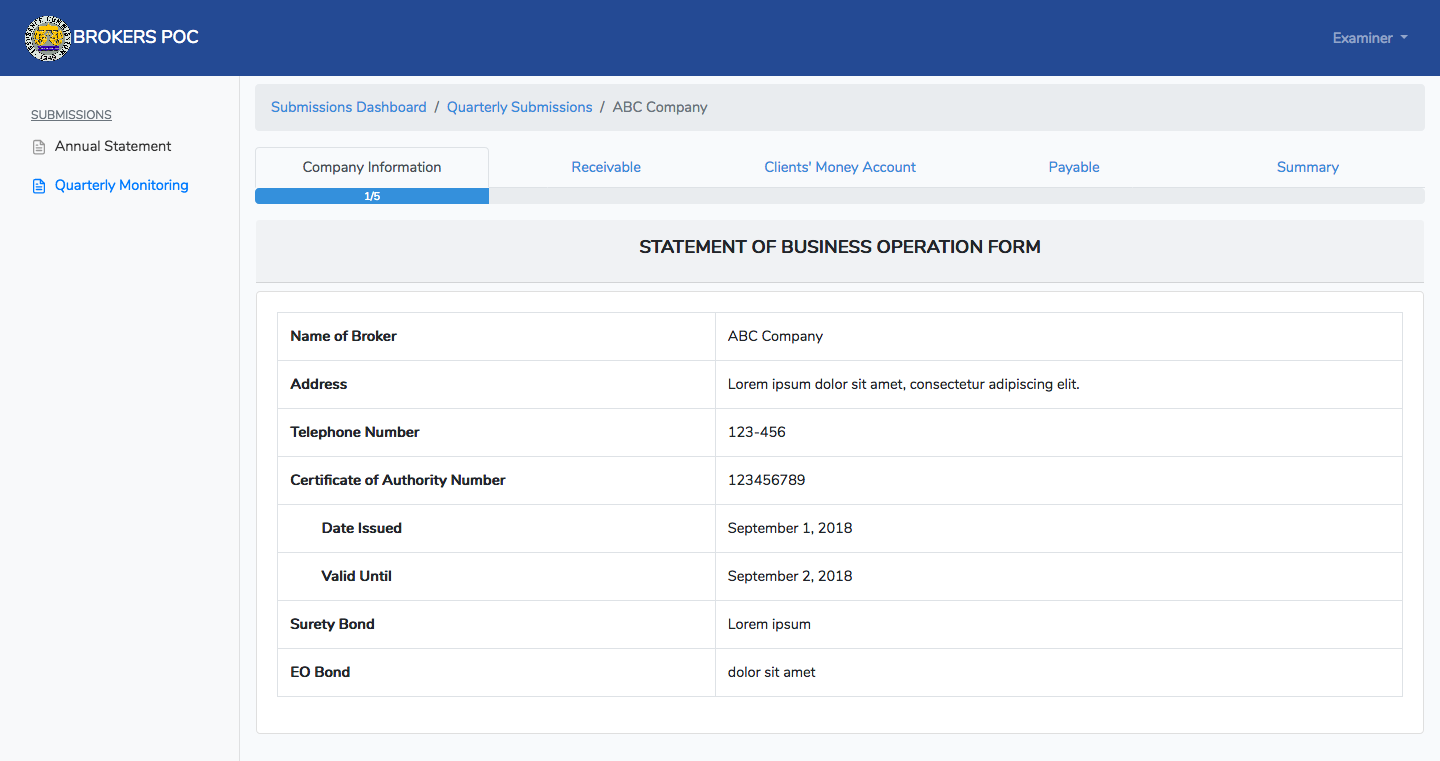
\includegraphics[keepaspectratio=true]{up-ic-screens/image70}{}\mdline{173}{}[\mdline{173}Examiner’s view\mdline{173}]\mdline{173} Like the company’s view, each section is
separated using tabs. This screen is the Company profile tab.%mdk

%mdk-data-line={180}
\mdline{180}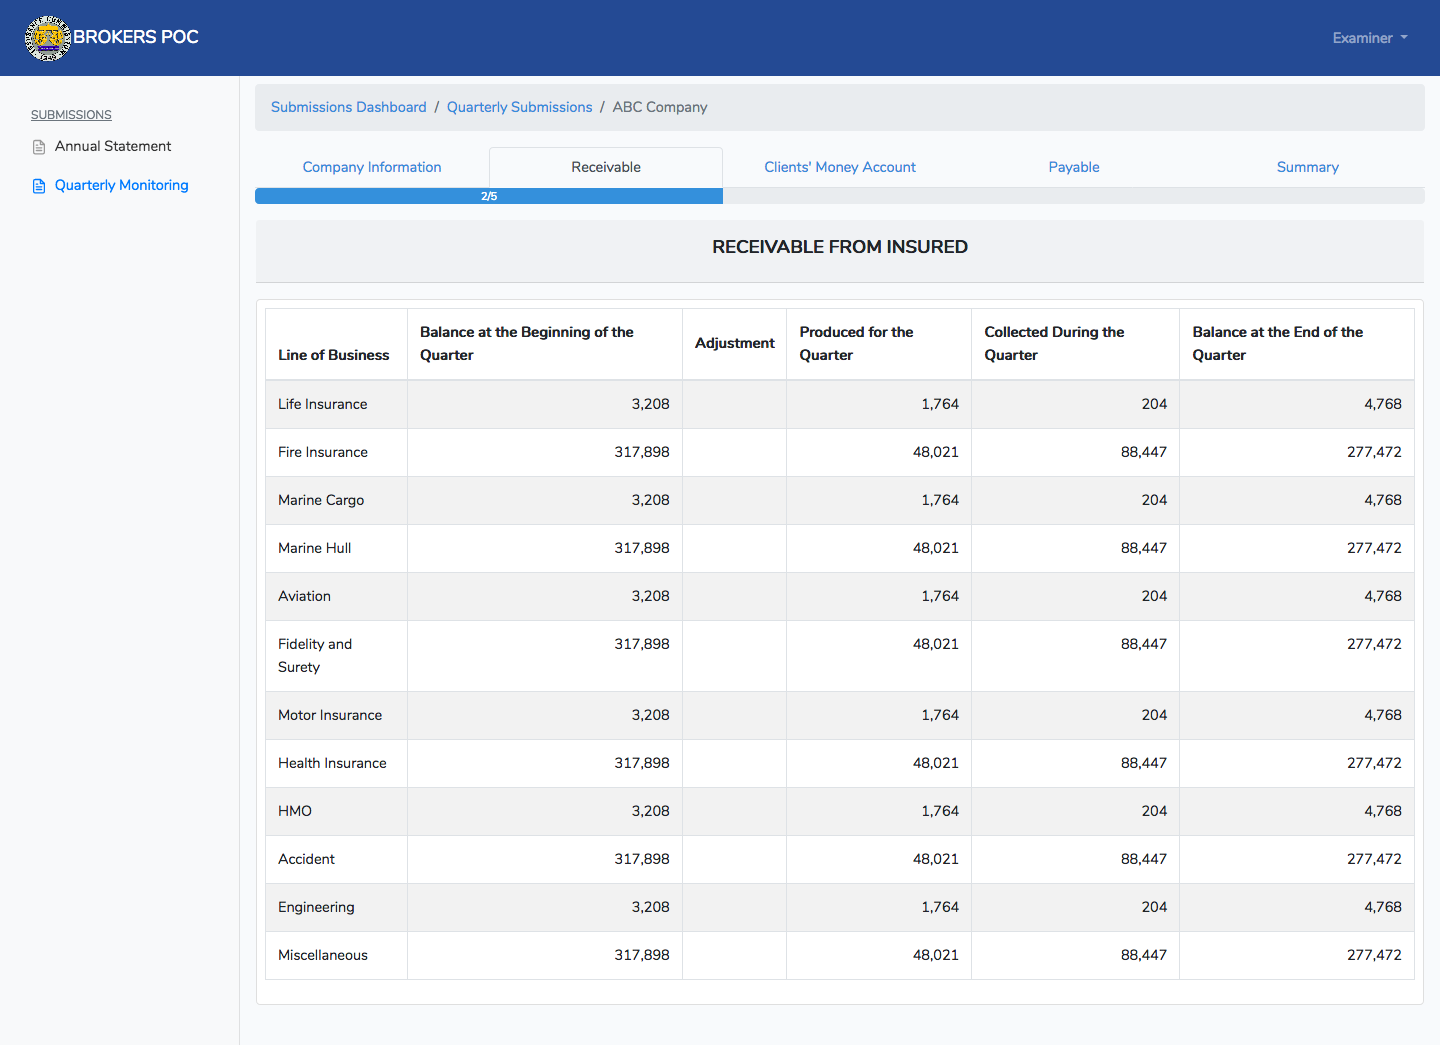
\includegraphics[keepaspectratio=true]{up-ic-screens/image189}{}\mdline{180}{}[\mdline{180}Examiner’s view\mdline{180}]\mdline{180} This is the receivable from insured
tab.%mdk

%mdk-data-line={185}
\mdline{185}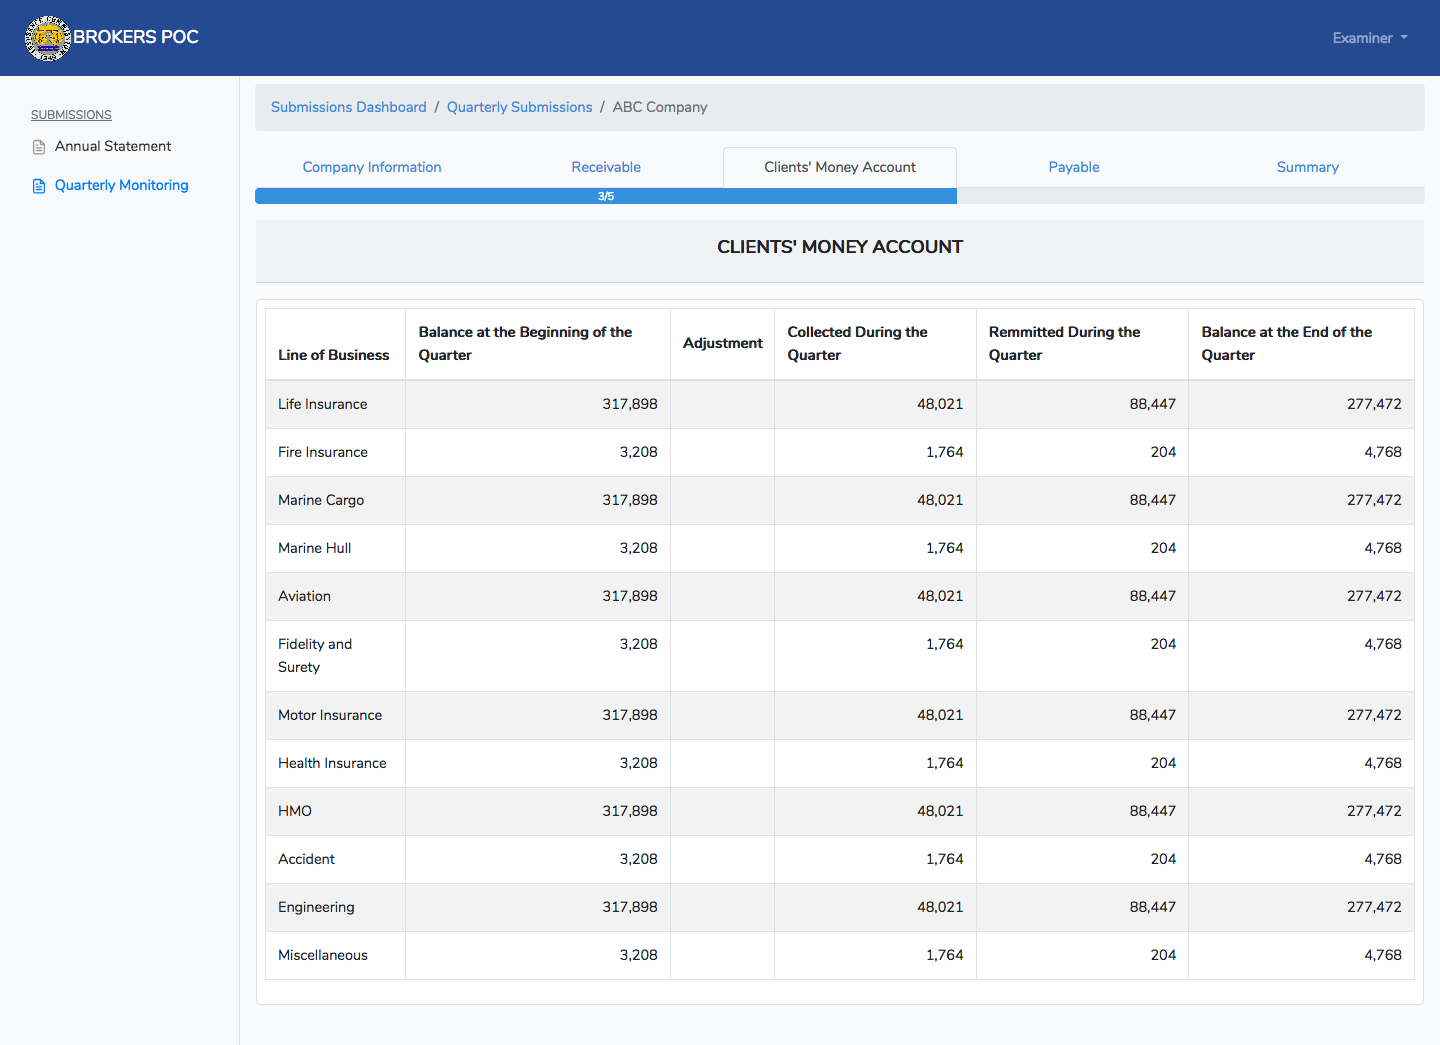
\includegraphics[keepaspectratio=true]{up-ic-screens/image5}{}\mdline{185}{}[\mdline{185}Examiner’s view\mdline{185}]\mdline{185} This is the Clients’ Money Account
tab.%mdk

%mdk-data-line={190}
\mdline{190}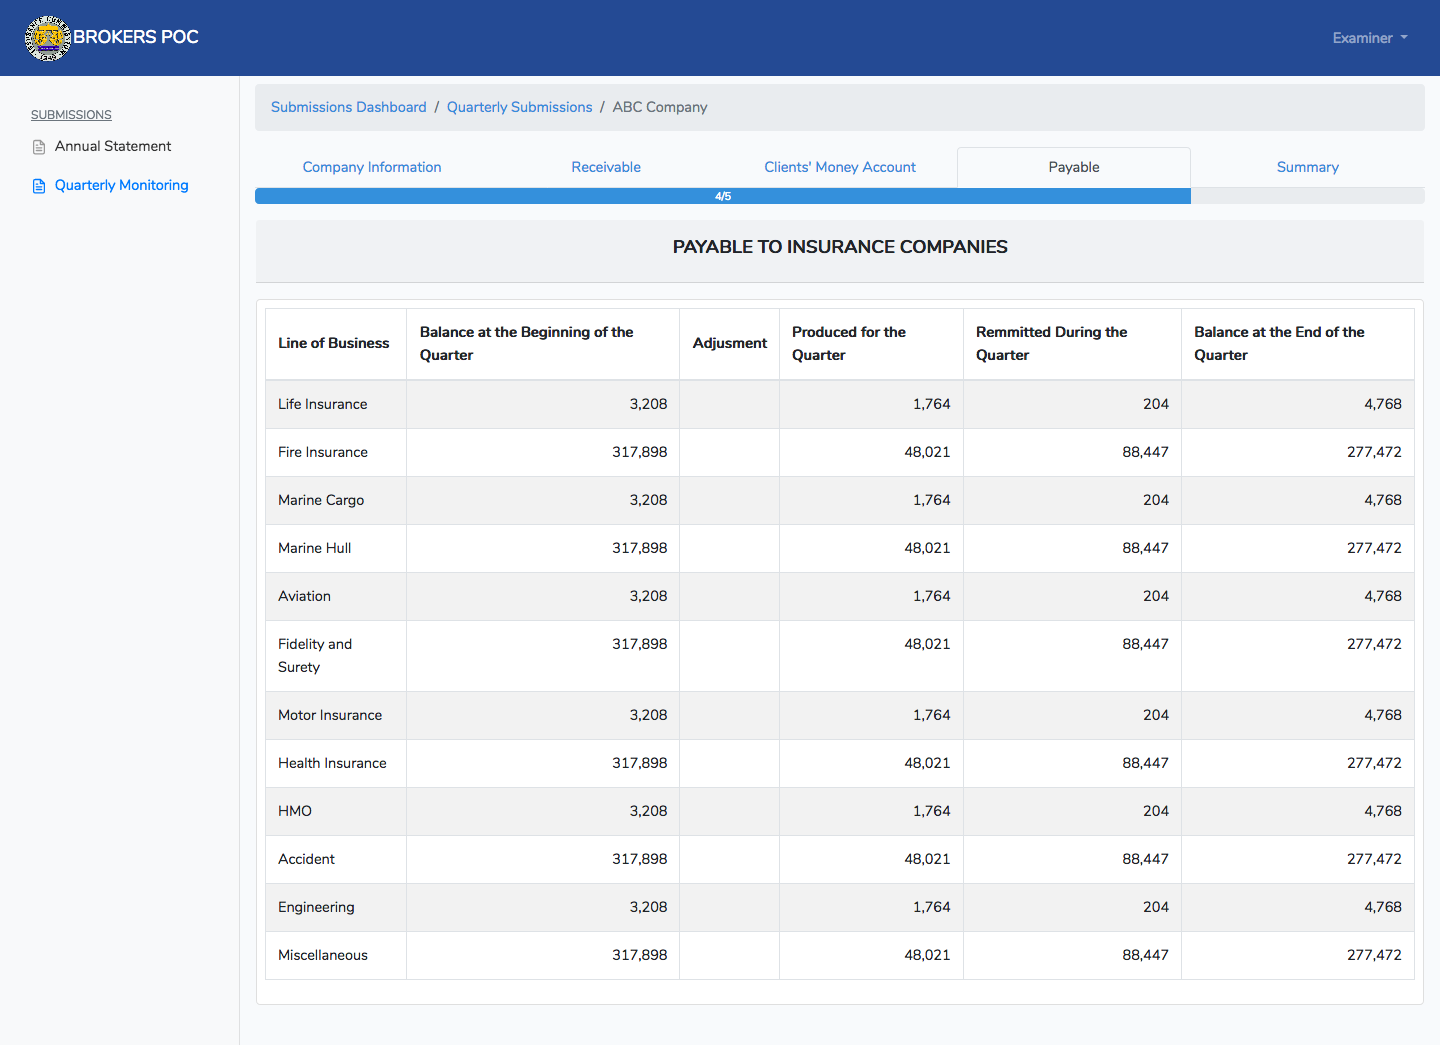
\includegraphics[keepaspectratio=true]{up-ic-screens/image175}{}\mdline{190}{}[\mdline{190}Examiner’s view\mdline{190}]\mdline{190} This is the Payable to Insurance Company
tab.%mdk

%mdk-data-line={195}
\mdline{195}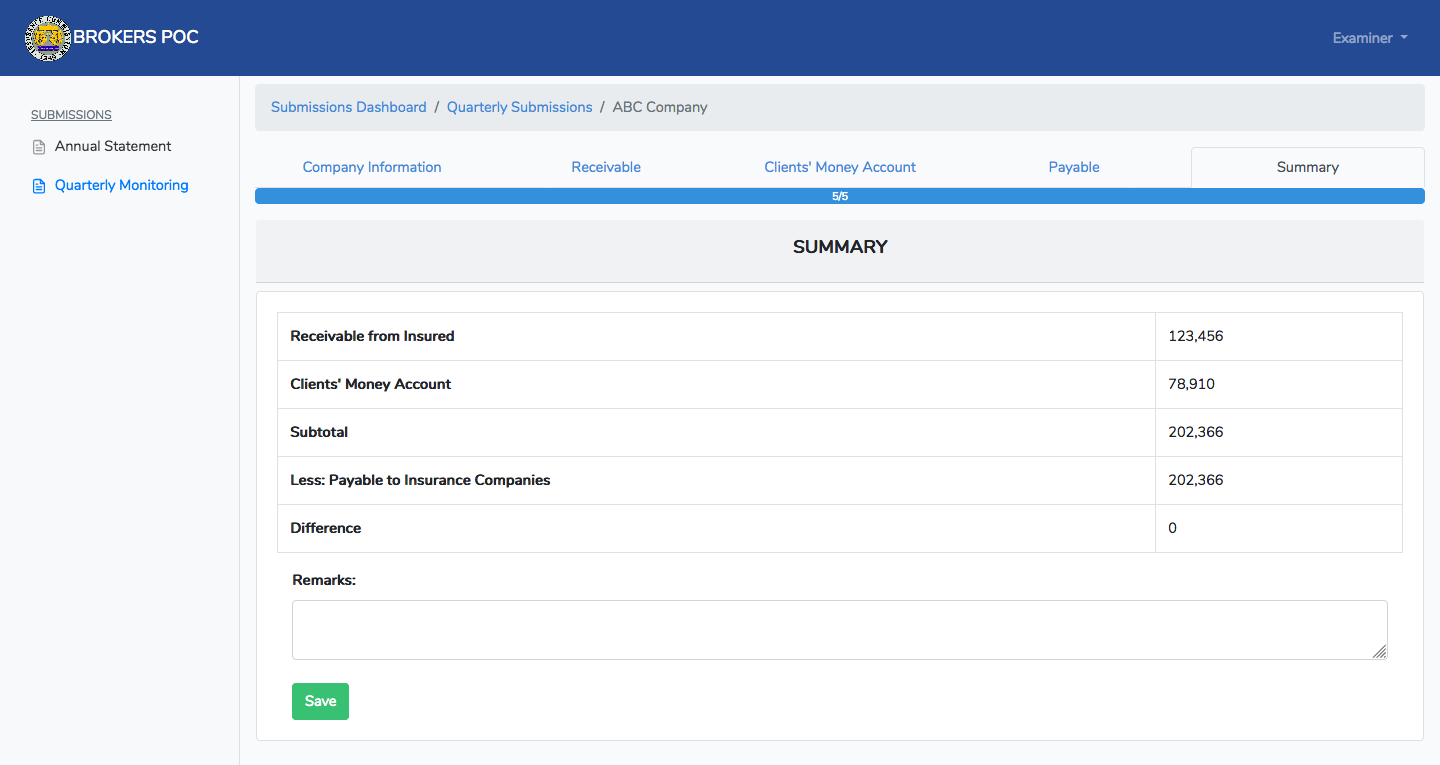
\includegraphics[keepaspectratio=true]{up-ic-screens/image12}{}\mdline{195}{}[\mdline{195}Examiner’s view\mdline{195}]\mdline{195} Lastly, this is the Summary tab. The
examiner can already view the details here\mdline{196} \mdline{196}- total Receivable from
insured (A), total Clients’ Money (B) , the sum of Receivable and
Clients’ Money (A+B), the total Payable to insurance company (C), the
difference between the sum of Receivable and Clients’ Money, and Payable
to insurance company (A+B-C). Finally, the examiner can put any remarks,
or comments, he/she needs to write.%mdk

%mdk-data-line={205}
\mdhr{}%mdk

%mdk-data-line={208}
\noindent\mdline{208}=============================%mdk

%mdk-data-line={210}
\subsection{\mdline{210}2.2.\hspace*{0.5em}\mdline{210}1.  HMO Division}\label{sec-1-hmo-division}%mdk%mdk

%mdk-data-line={213}
\noindent\mdline{213}{}[\mdline{213}Company View\mdline{213}]\mdline{213} Below is the the company dashboard.
Shown are the processes accessible by companies.%mdk

%mdk-data-line={216}
\mdline{216}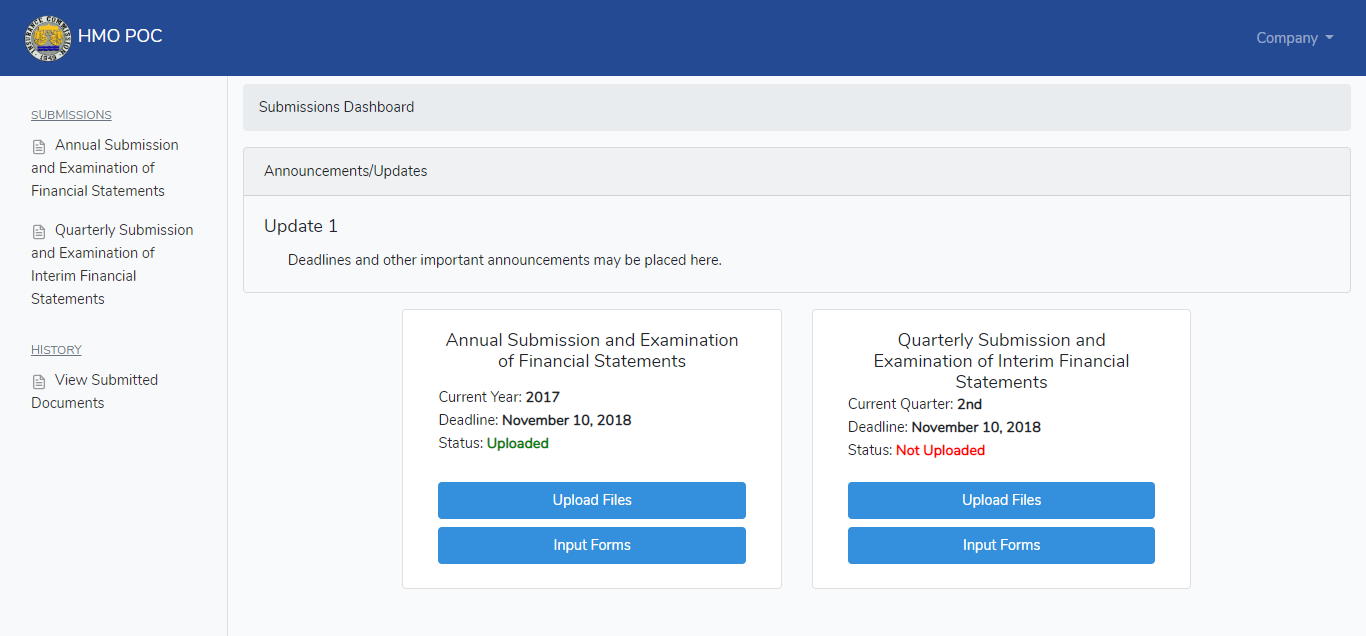
\includegraphics[keepaspectratio=true]{up-ic-screens/image197}{}\mdline{216}%mdk

%mdk-data-line={218}
\mdline{218}{}[\mdline{218}Examiner View\mdline{218}]\mdline{218} Below is the examiner dashboard.
Shown are the submissions made by companies.%mdk

%mdk-data-line={221}
\mdline{221}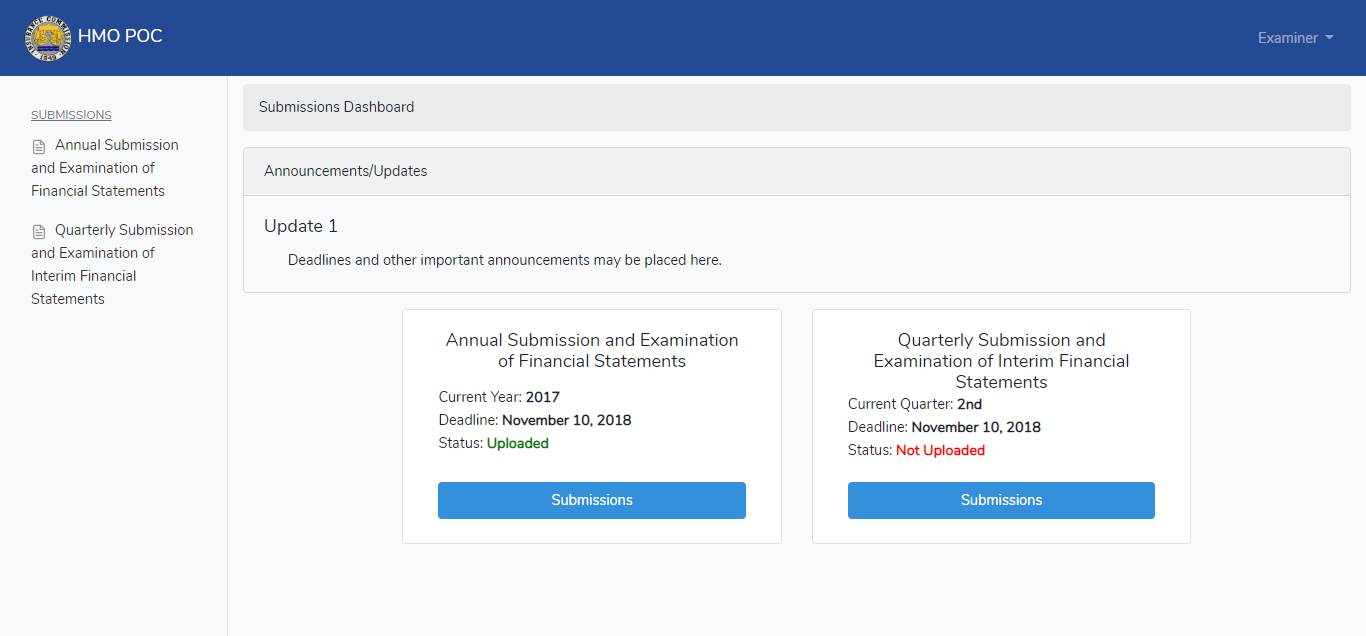
\includegraphics[keepaspectratio=true]{up-ic-screens/image179}{}\mdline{221}%mdk

%mdk-data-line={223}
\begin{enumerate}[noitemsep,topsep=\mdcompacttopsep]%mdk

%mdk-data-line={223}
\item{}
%mdk-data-line={223}
\subsubsection{\mdline{223}2.2.1.\hspace*{0.5em}\mdline{223}Annual Submission and Examination of Financial Statements}\label{sec-annual-submission-and-examination-of-financial-statements}%mdk%mdk%mdk
%mdk
\end{enumerate}%mdk

%mdk-data-line={225}
\noindent\mdline{225}{}[\mdline{225}Company View\mdline{225}]\mdline{225} Below is where companies can upload
their files for the annual submission.%mdk

%mdk-data-line={228}
\mdline{228}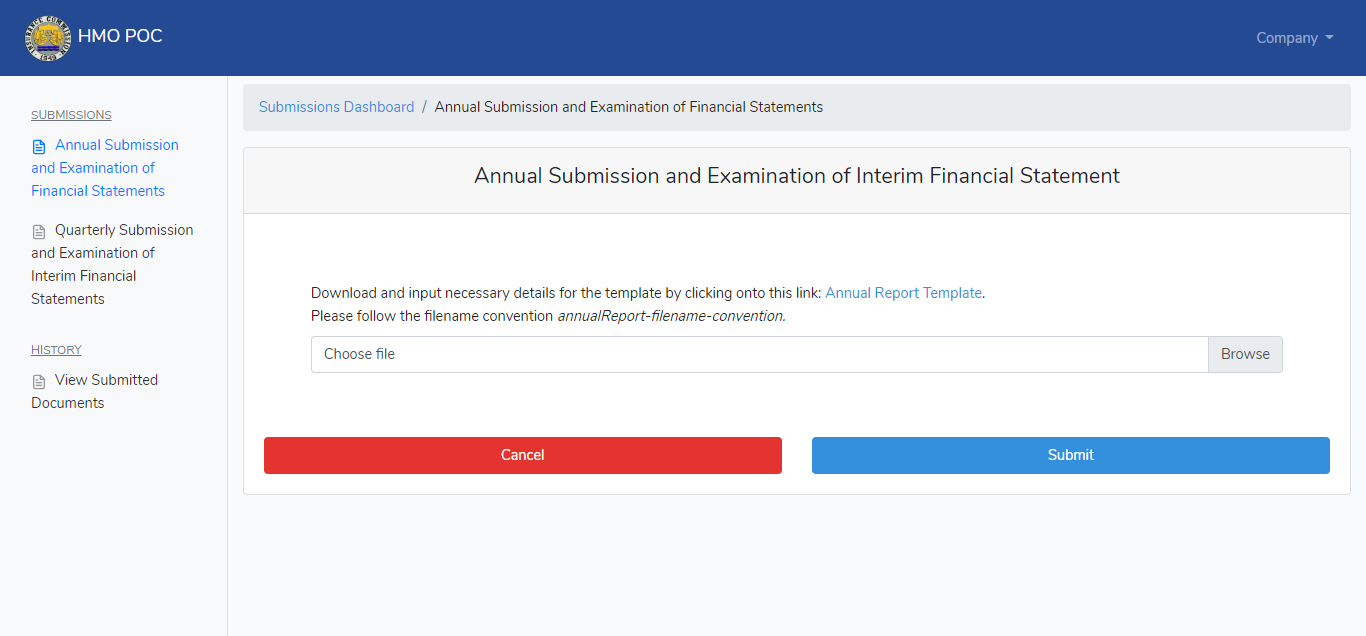
\includegraphics[keepaspectratio=true]{up-ic-screens/image87}{}\mdline{228}%mdk

%mdk-data-line={230}
\mdline{230}{}[\mdline{230}Company View\mdline{230}]\mdline{230} Below are the forms for companies to
fill out which are tabbed as SFP and SCI for annual submissions.%mdk

%mdk-data-line={233}
\mdline{233}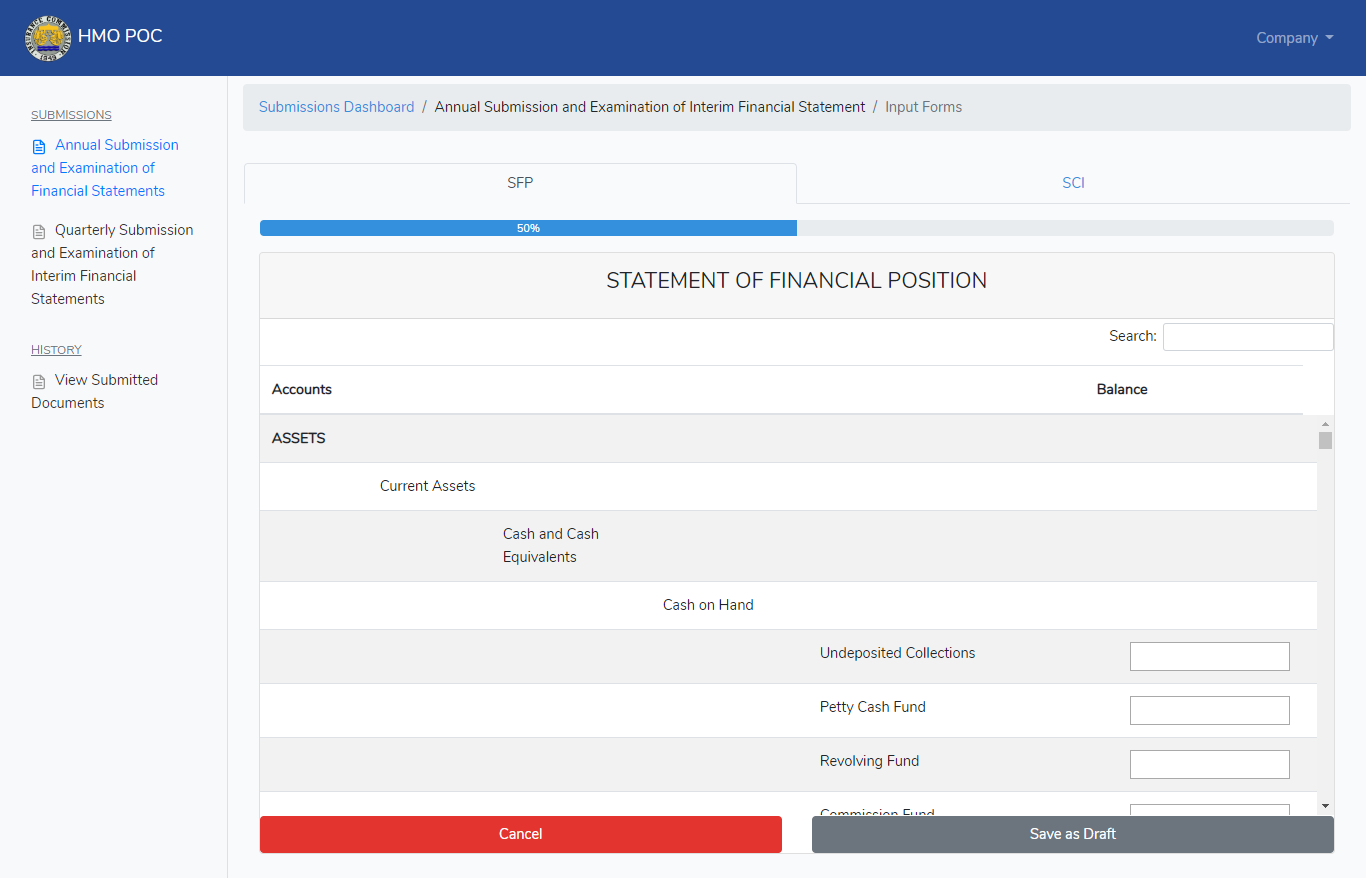
\includegraphics[keepaspectratio=true]{up-ic-screens/image217}{}\mdline{233}%mdk

%mdk-data-line={235}
\mdline{235}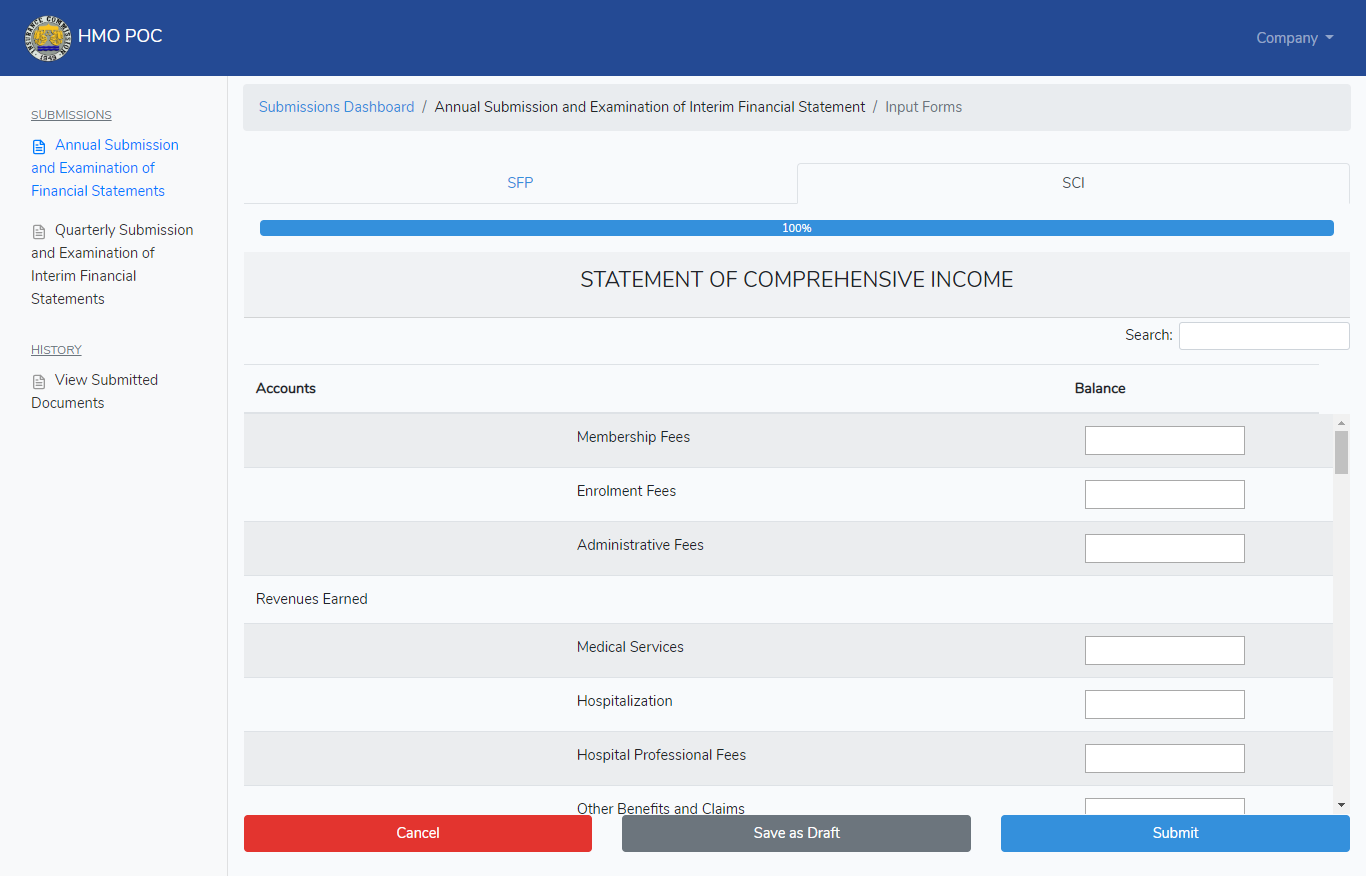
\includegraphics[keepaspectratio=true]{up-ic-screens/image115}{}\mdline{235}%mdk

%mdk-data-line={237}
\mdline{237}{}[\mdline{237}Examiner View\mdline{237}]\mdline{237} Below is the submissions by companies
for annual reports.%mdk

%mdk-data-line={240}
\mdline{240}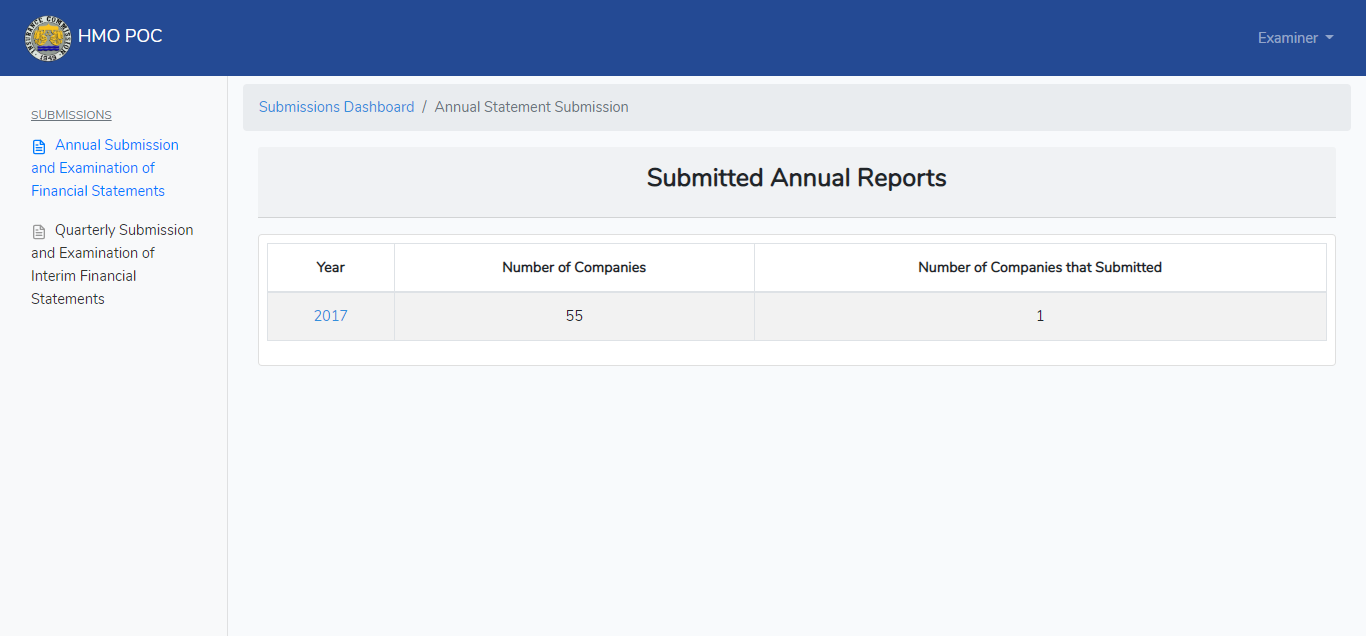
\includegraphics[keepaspectratio=true]{up-ic-screens/image53}{}\mdline{240}%mdk

%mdk-data-line={242}
\begin{enumerate}[noitemsep,topsep=\mdcompacttopsep]%mdk

%mdk-data-line={242}
\item{}
%mdk-data-line={242}
\subsubsection{\mdline{242}2.2.2.\hspace*{0.5em}\mdline{242}Quarterly Submission and Examination of Interim Financial Statements}\label{sec-quarterly-submission-and-examination-of-interim-financial-statements}%mdk%mdk%mdk
%mdk
\end{enumerate}%mdk

%mdk-data-line={244}
\noindent\mdline{244}{}[\mdline{244}Company View\mdline{244}]\mdline{244} Below is where companies can upload their files
for quarterly submission\mdline{245}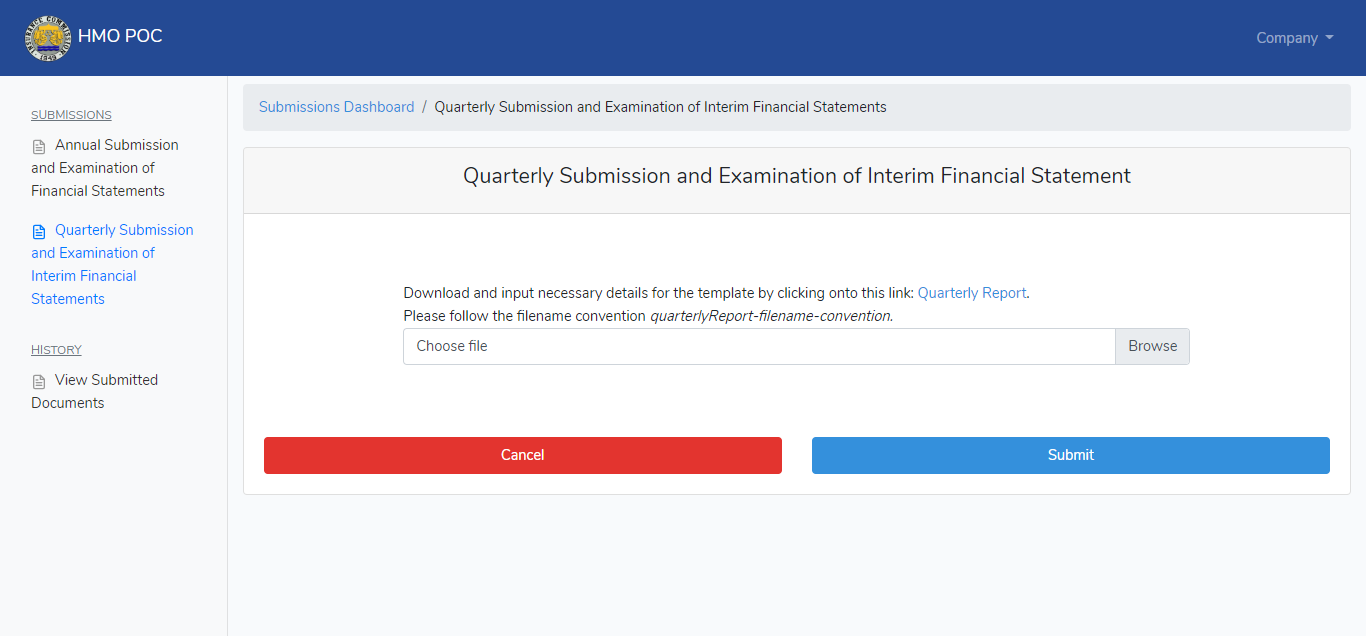
\includegraphics[keepaspectratio=true]{up-ic-screens/image167}{}\mdline{245}%mdk

%mdk-data-line={247}
\mdline{247}{}[\mdline{247}Company View\mdline{247}]\mdline{247} Below are the forms for companies to
fill out which are tabbed as SFP and SCI for quarterly submissions.%mdk

%mdk-data-line={251}
\mdline{251}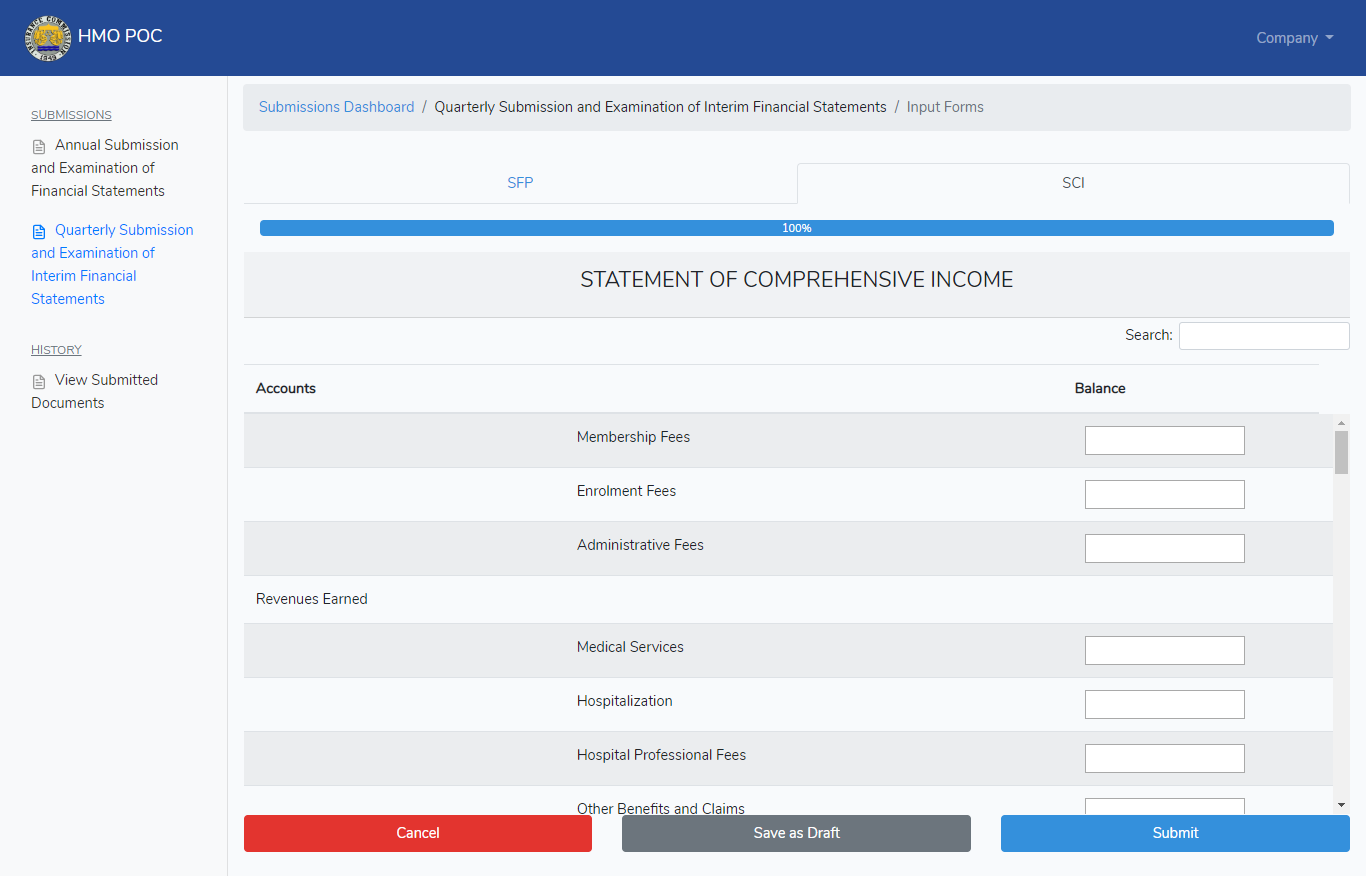
\includegraphics[keepaspectratio=true]{up-ic-screens/image116}{}\mdline{251}%mdk

%mdk-data-line={253}
\mdline{253}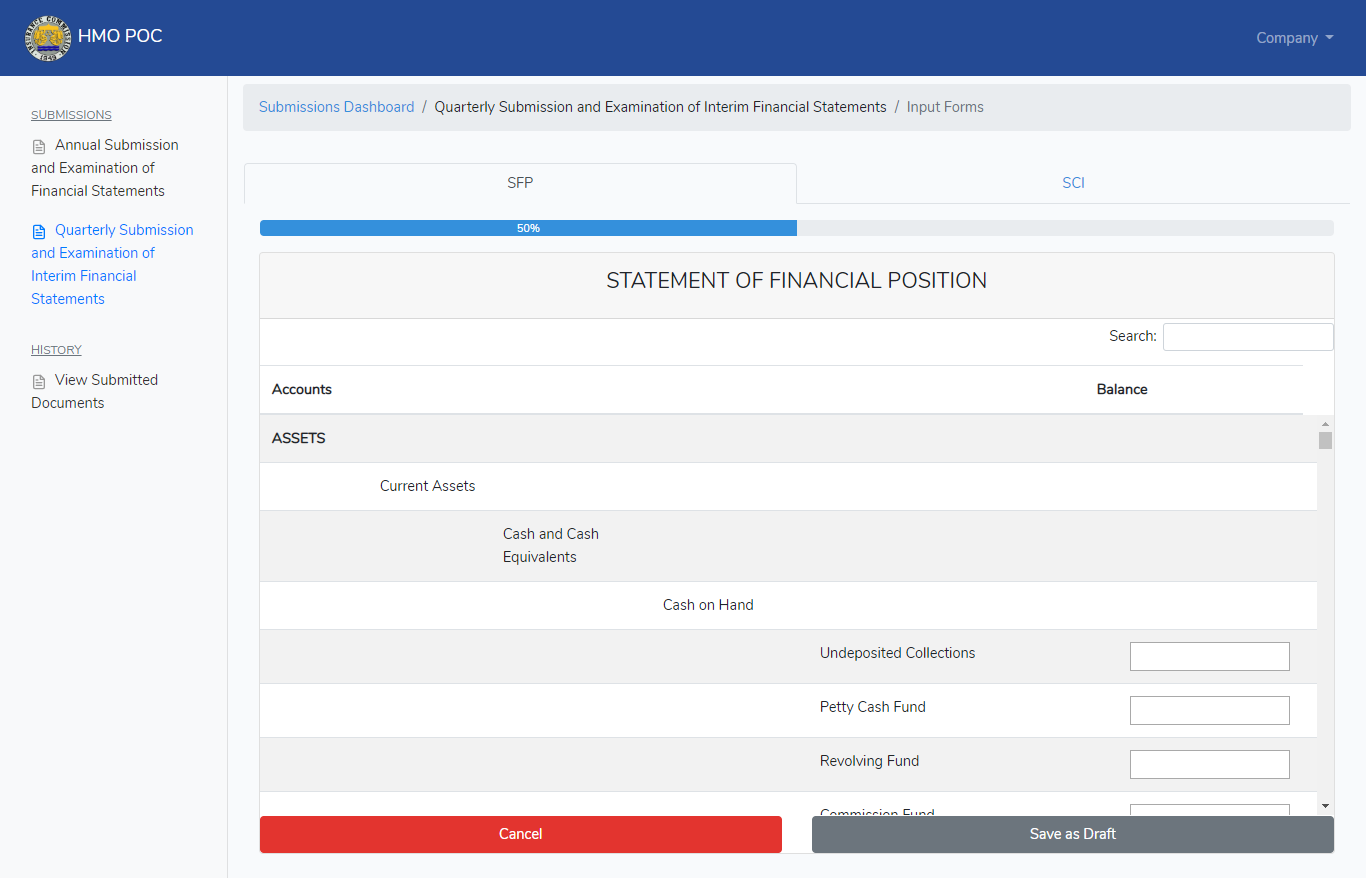
\includegraphics[keepaspectratio=true]{up-ic-screens/image211}{}\mdline{253}%mdk

%mdk-data-line={255}
\mdline{255}{}[\mdline{255}Examiner View\mdline{255}]\mdline{255} Below are the quarterly submissions
by companies summarized and individual company view,
respectively.%mdk

%mdk-data-line={259}
\mdline{259}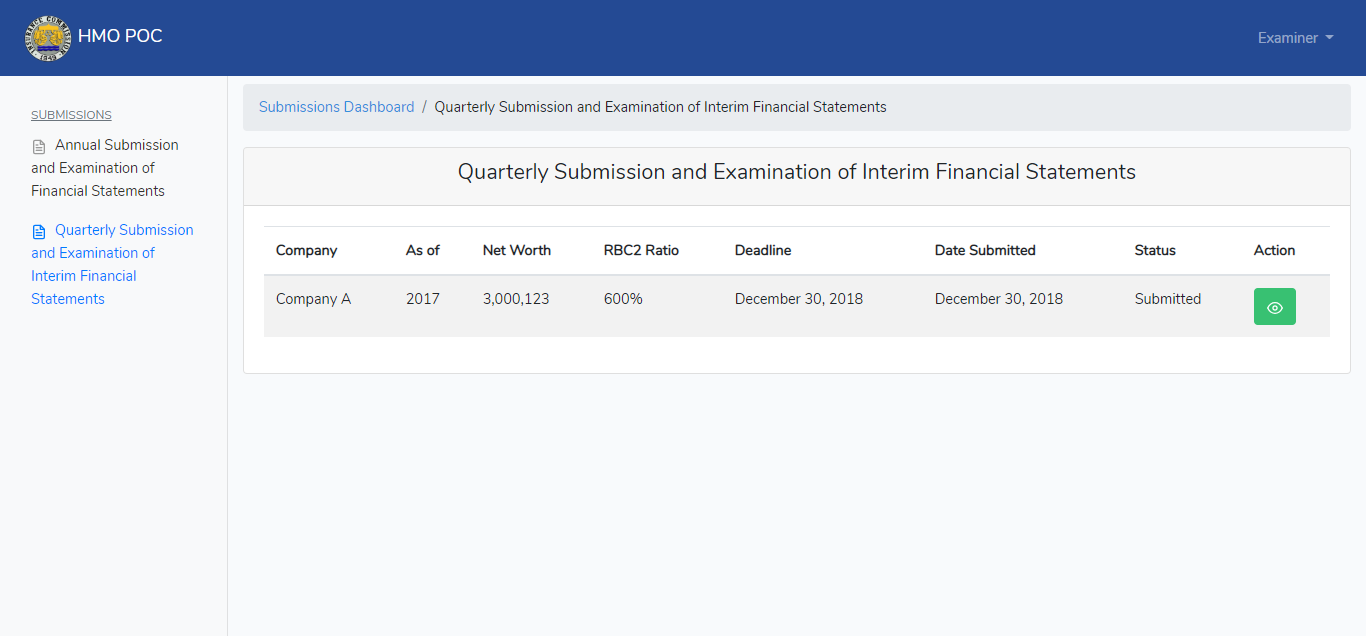
\includegraphics[keepaspectratio=true]{up-ic-screens/image125}{}\mdline{259}%mdk

%mdk-data-line={261}
\mdline{261}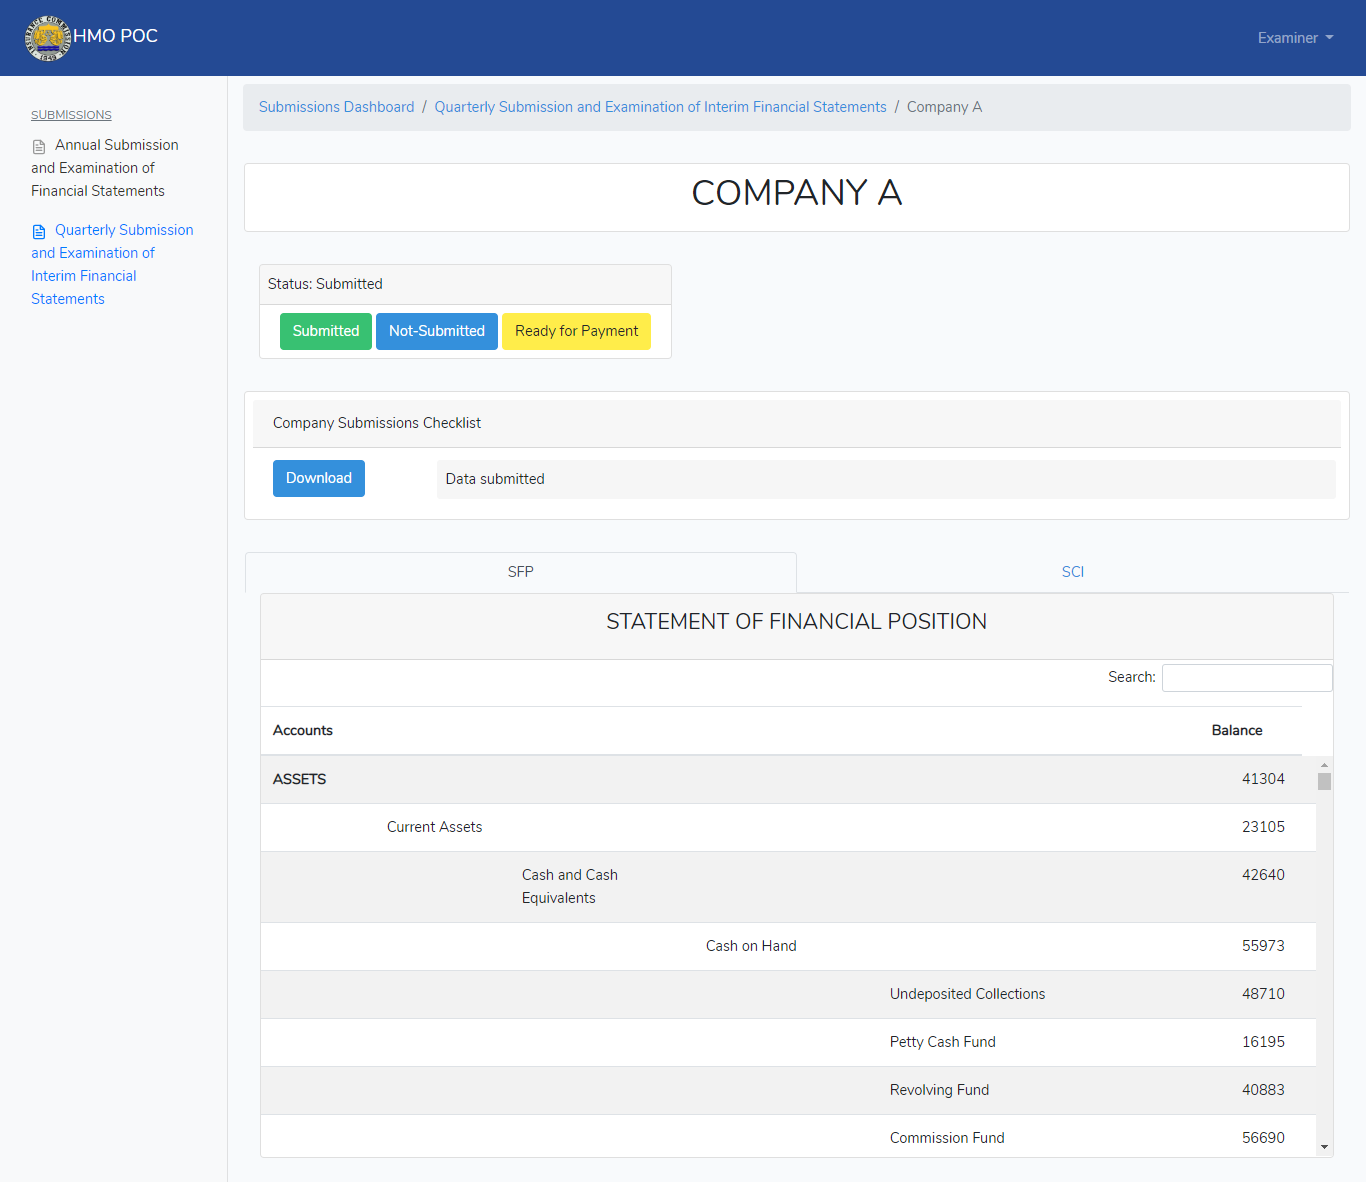
\includegraphics[keepaspectratio=true]{up-ic-screens/image96}{}\mdline{261}%mdk

%mdk-data-line={263}
\mdhr{}%mdk

%mdk-data-line={266}
\noindent\mdline{266}=============================%mdk

%mdk-data-line={268}
\subsection{\mdline{268}2.3.\hspace*{0.5em}\mdline{268}1.  Life/ MBA/ Trust Division}\label{sec-1-life-mba-trust-division}%mdk%mdk

%mdk-data-line={273}
\begin{enumerate}[noitemsep,topsep=\mdcompacttopsep]%mdk

%mdk-data-line={273}
\item{}
%mdk-data-line={273}
\subsubsection{\mdline{273}2.3.1.\hspace*{0.5em}\mdline{273}Annual Submission and Examination of Financial Standing of Life Companies with Separate Presentation for Composite Insurance Companies}\label{sec-annual-submission-and-examination-of-financial-standing-of-life-companies-with-separate-presentation-for-composite-insurance-companies}%mdk%mdk%mdk
%mdk
\end{enumerate}%mdk

%mdk-data-line={277}
\noindent\mdline{277}Company View%mdk

%mdk-data-line={279}
\mdline{279}This page will appear upon logging in a company
account. The page consist of a sidebar on the left side, a navigation
bar above with the insurance commission logo and a specified label, if
any. On the middle, it has the dashboard which has the
announcements/updates regarding submissions of documents. There\mdline{283}'\mdline{283}s also
the cards which are consisting of all the submissions needed by the
companies. Each card consist of the Document submission header, current
quarter of submission, its deadline and status of the company on
submission. Beside the document submission header is a question icon
which pops up a modal when clicked that consist of requirements,
guidelines and circular letters for that specific submission.%mdk

%mdk-data-line={291}
\mdline{291}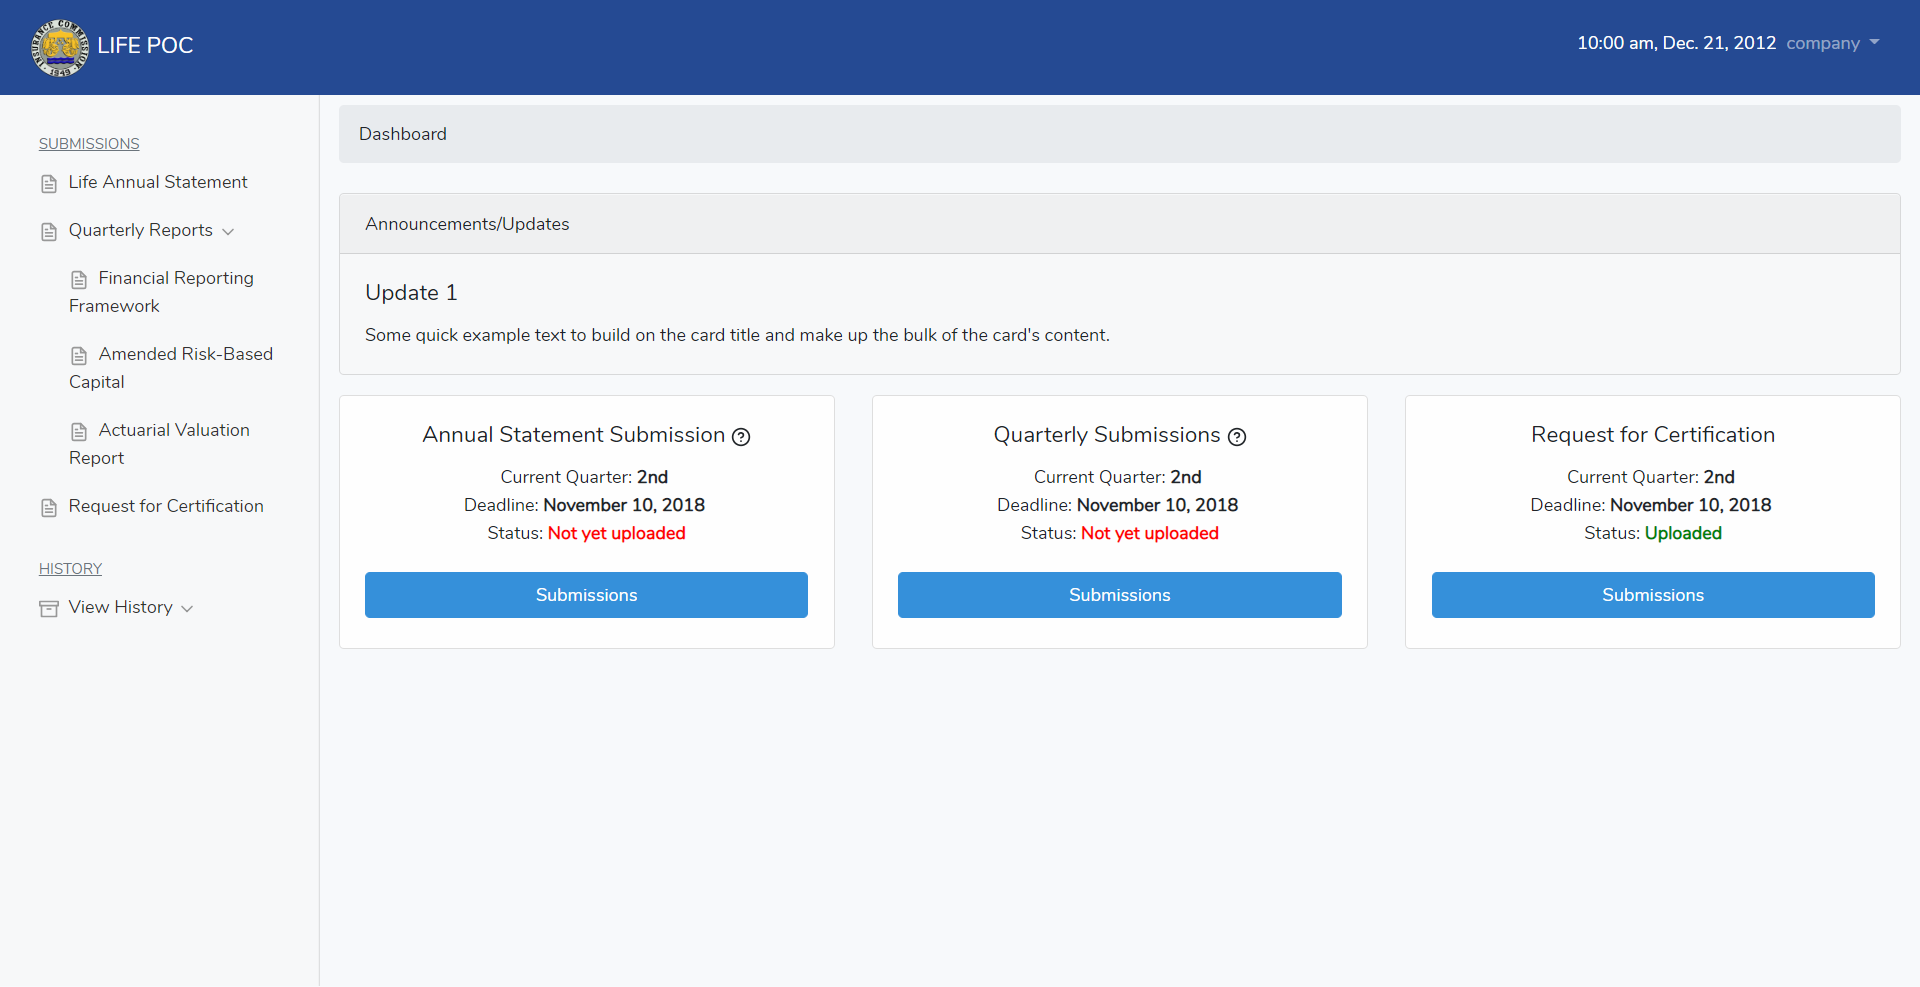
\includegraphics[keepaspectratio=true]{up-ic-screens/image111}{}\mdline{291}%mdk

%mdk-data-line={295}
\mdhr{}%mdk

%mdk-data-line={299}
\noindent\mdline{299}Upon clicking the Annual Submission card or the Annual
Statement from the sidebar, it will redirect to this page. Here, the
company can upload the required documents based on the checklist
provided by the insurance commission. Each file submission has specific
file type allowed. Once the required documents are passed, It will be
checked. The submit button is blocked out until all required documents
are uploaded. The company can also save as draft to continue uploading
later.%mdk

%mdk-data-line={308}
\mdline{308}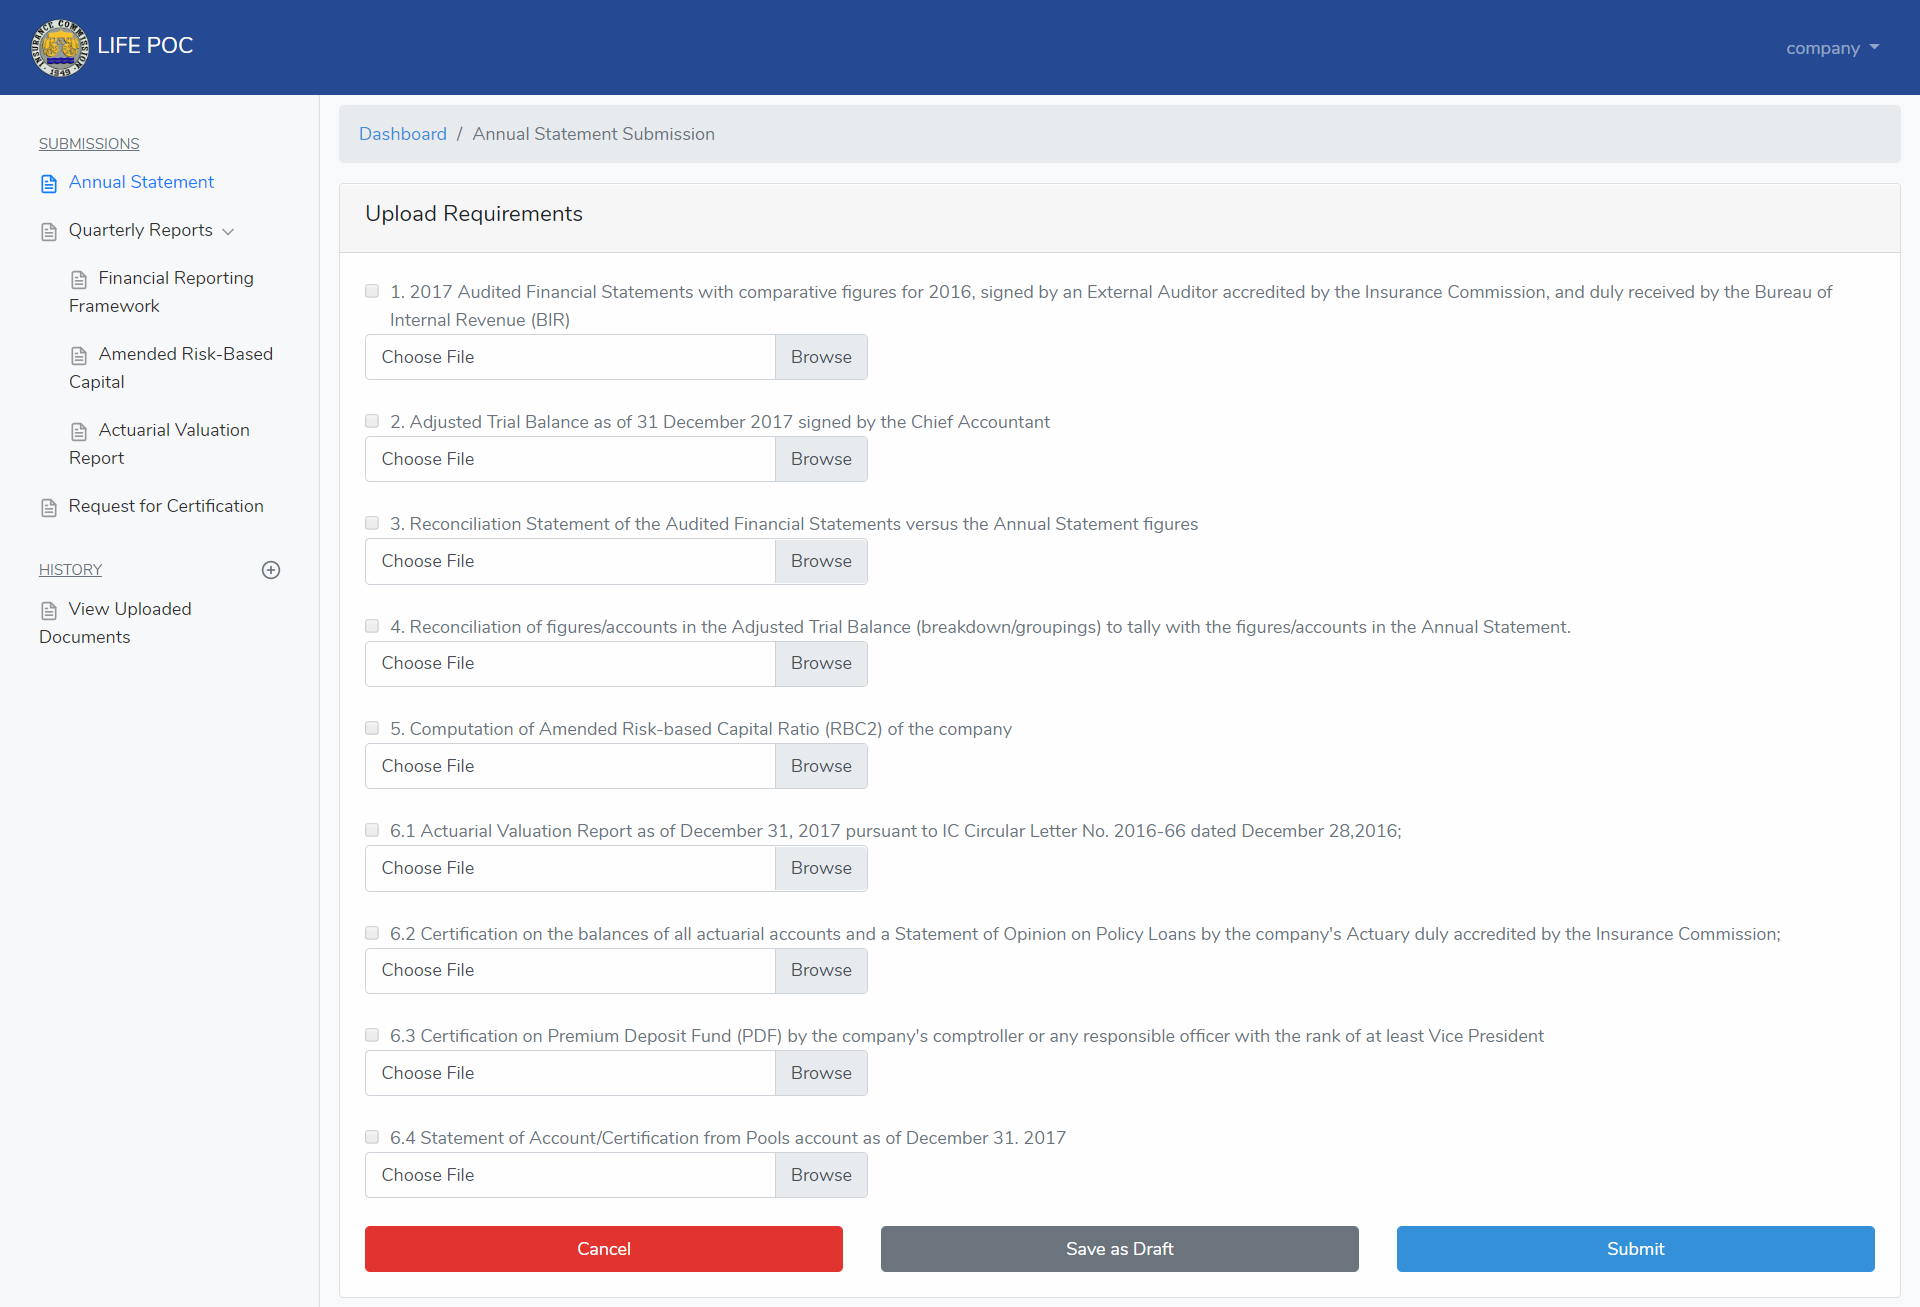
\includegraphics[keepaspectratio=true]{up-ic-screens/image64}{}\mdline{308}%mdk

%mdk-data-line={310}
\mdhr{}%mdk

%mdk-data-line={314}
\noindent\mdline{314}Upon clicking View History on the sidebar, the user is
given an option to which division submission it wants to view. In this
specific web screen, It can choose to view all its submissions to Life
division. The main page has tables which are divided based on the
deadlines of each processes. Each tables can be sorted and filtered to
be able to track if they have submitted the documents.%mdk

%mdk-data-line={321}
\mdline{321}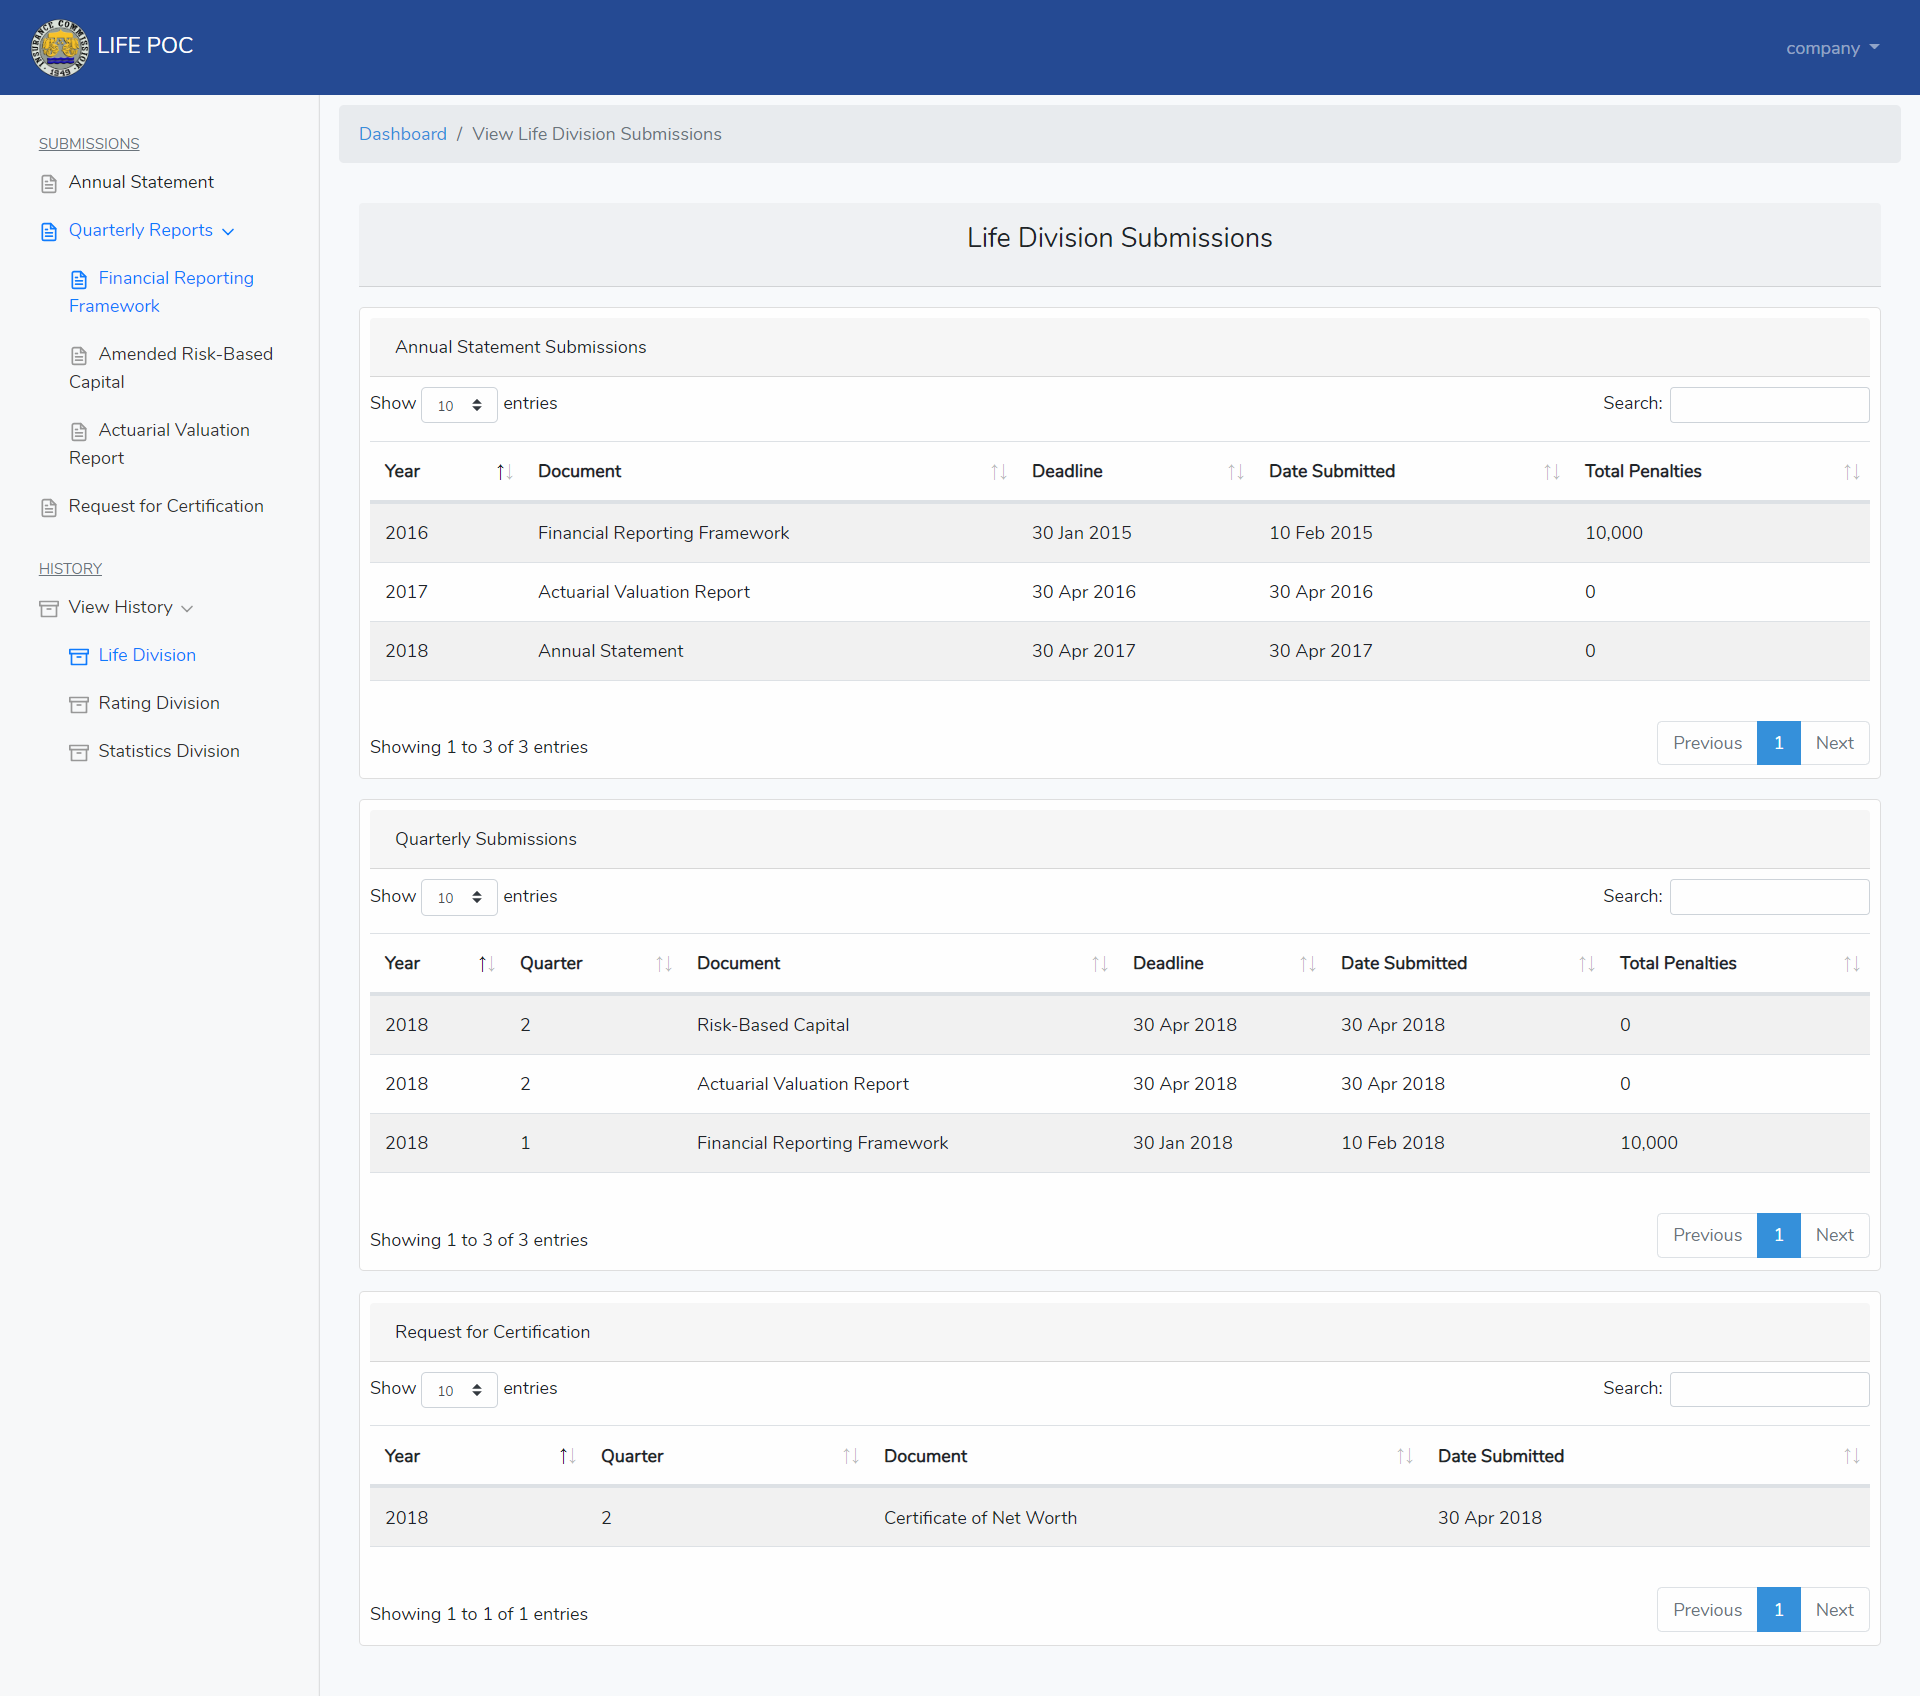
\includegraphics[keepaspectratio=true]{up-ic-screens/image99}{}\mdline{321}%mdk

%mdk-data-line={325}
\mdhr{}%mdk

%mdk-data-line={329}
\noindent\mdline{329}Examiner View%mdk

%mdk-data-line={331}
\mdline{331}This page will appear upon logging in an examiner
account of insurance commission. The page consist of a sidebar on the
left side, a navigation bar above with the insurance commission logo and
a specified label, if any. On the middle, it has the dashboard which has
the cards which are consisting of all the submissions needed to be done
by the companies. Each card consist of the Document submission header,
current quarter of submission and its deadline. Beside the document
submission header is a question icon which pops up a modal when clicked
that consist of requirements, guidelines and circular letters for that
specific submission. Below the page is a table of certificate requests.
The examiner can view incoming requests for certification of companies
through a table. The examiner can then take action on each request by
viewing it.%mdk

%mdk-data-line={345}
\mdhr{}%mdk

%mdk-data-line={347}
\noindent\mdline{347}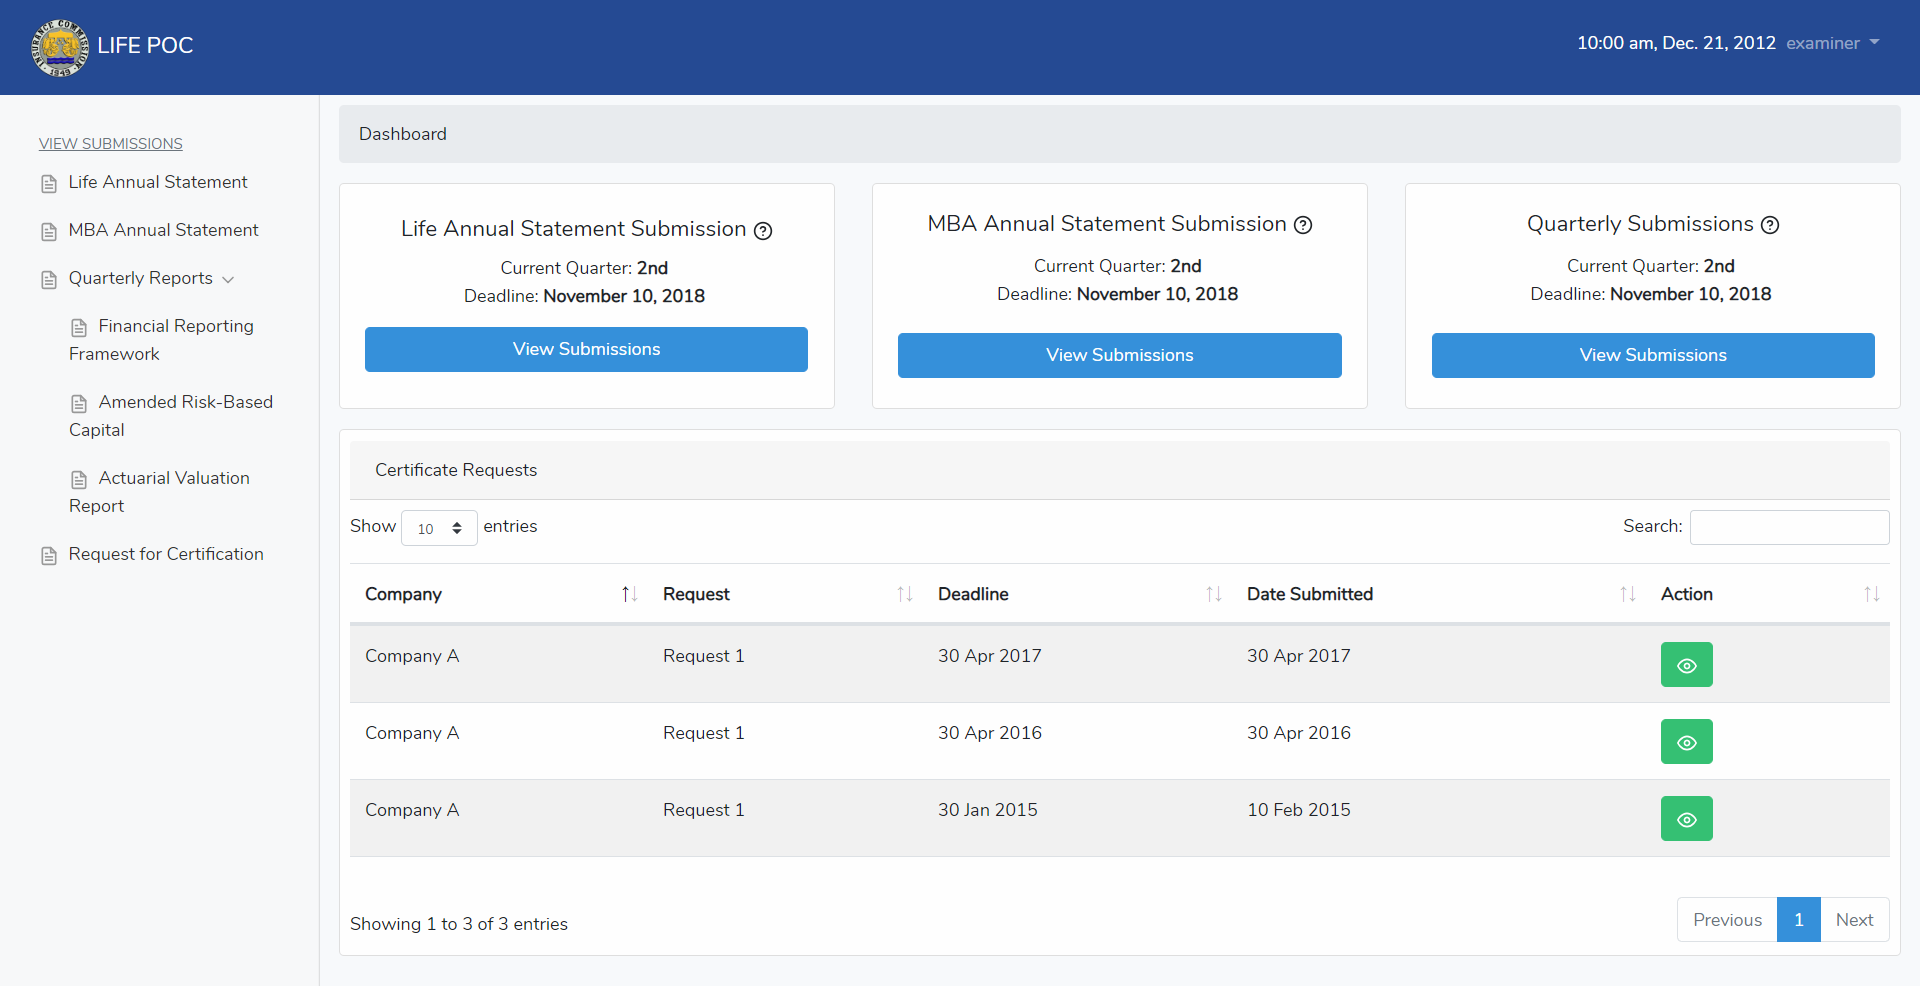
\includegraphics[keepaspectratio=true]{up-ic-screens/image47}{}\mdline{347}%mdk

%mdk-data-line={349}
\mdline{349}Upon clicking the Annual Submission card or the Annual
Statement from the sidebar, the examiner will be redirected to the page
with company list. The table with company list shows important
informations needed immediately for viewing. An examiner can also take
action of viewing the company submission in a much detailed form.%mdk

%mdk-data-line={355}
\paragraph{\mdline{355}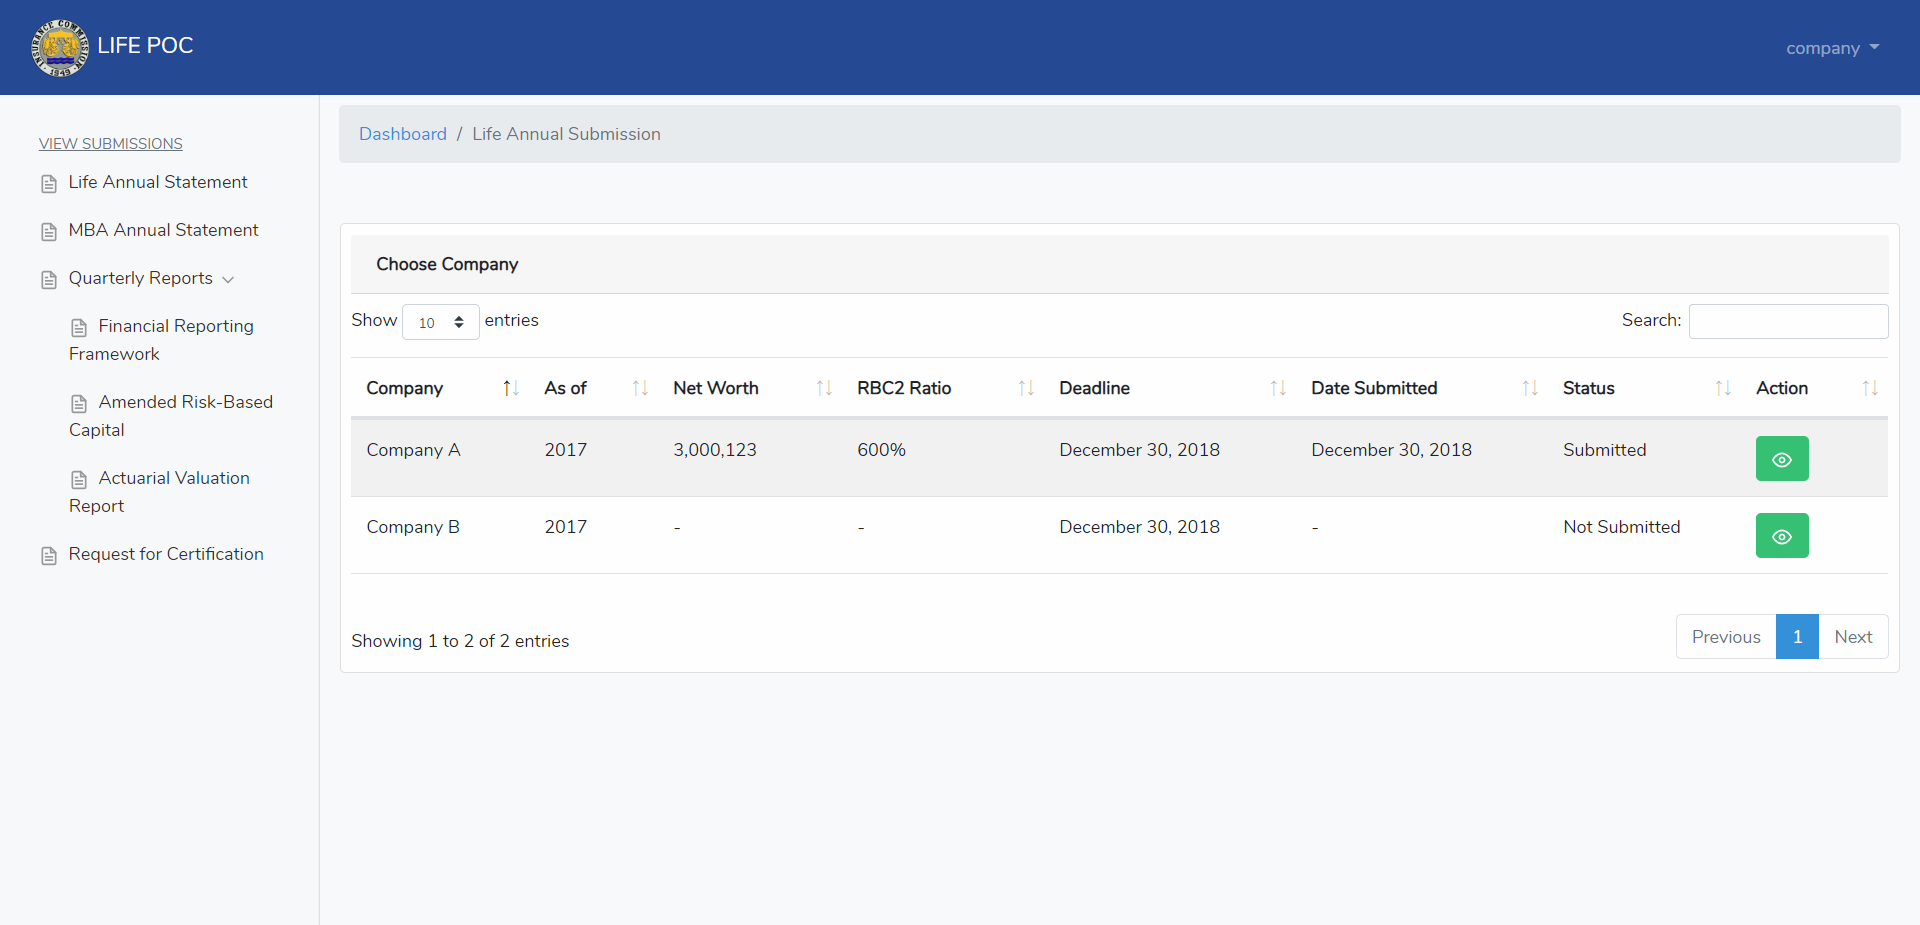
\includegraphics[keepaspectratio=true]{up-ic-screens/image95}{}}\label{sec-up-ic-screensimage95png}%mdk%mdk

%mdk-data-line={357}
\paragraph{\mdline{357} }\label{sec--}%mdk%mdk

%mdk-data-line={359}
\paragraph{\mdline{359} }\label{sec--}%mdk%mdk

%mdk-data-line={361}
\paragraph{\mdline{361} }\label{sec--}%mdk%mdk

%mdk-data-line={363}
\paragraph{\mdline{363} }\label{sec--}%mdk%mdk

%mdk-data-line={365}
\paragraph{\mdline{365} }\label{sec--}%mdk%mdk

%mdk-data-line={367}
\paragraph{\mdline{367} }\label{sec--}%mdk%mdk

%mdk-data-line={369}
\paragraph{\mdline{369} }\label{sec--}%mdk%mdk

%mdk-data-line={371}
\paragraph{\mdline{371} }\label{sec--}%mdk%mdk

%mdk-data-line={373}
\paragraph{\mdline{373} }\label{sec--}%mdk%mdk

%mdk-data-line={409}
\noindent\mdline{409}Upon clicking the view button, the examiner will be
directed to the page where you can change the status of the submission,
download the submitted checklist, and company files.%mdk

%mdk-data-line={413}
\paragraph{\mdline{413}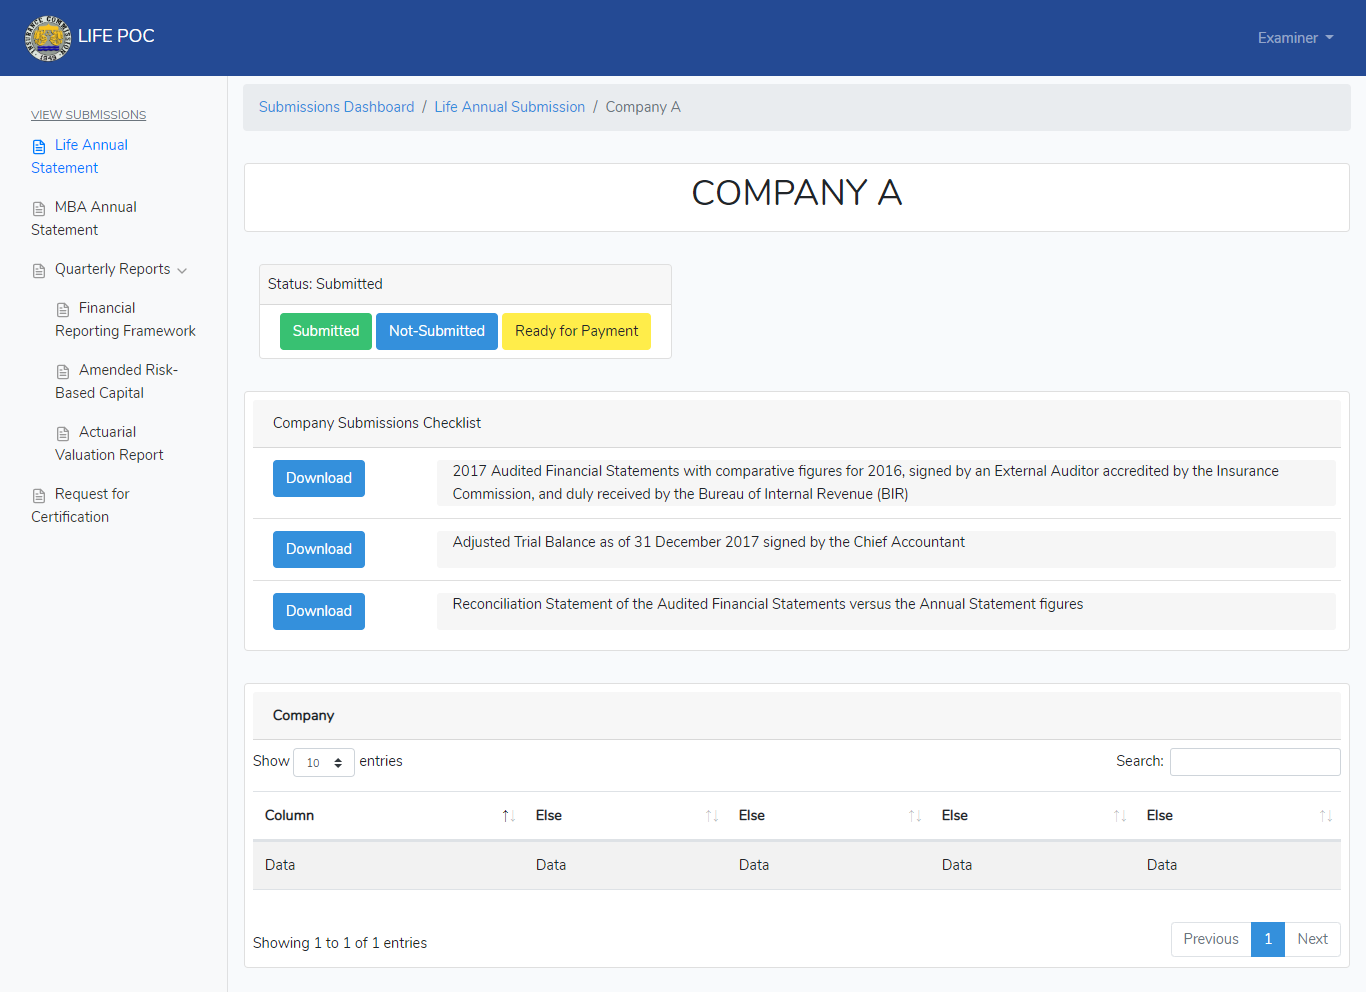
\includegraphics[keepaspectratio=true]{up-ic-screens/image129}{}}\label{sec-up-ic-screensimage129png}%mdk%mdk

%mdk-data-line={419}
\noindent\mdline{419}Note: Upon clicking the view icon the computation for
net worth will be shown%mdk

%mdk-data-line={424}
\begin{enumerate}[noitemsep,topsep=\mdcompacttopsep]%mdk

%mdk-data-line={424}
\item{}
%mdk-data-line={424}
\subsubsection{\mdline{424}2.3.2.\hspace*{0.5em}\mdline{424}Annual Submission and Examination of Mutual Benefit Association (MBA)}\label{sec-annual-submission-and-examination-of-mutual-benefit-association-mba}%mdk%mdk%mdk
%mdk
\end{enumerate}%mdk

%mdk-data-line={428}
\noindent\mdline{428}Company View%mdk

%mdk-data-line={430}
\mdline{430}This page will appear upon logging in a company
account. The page consist of a sidebar on the left side, a navigation
bar above with the insurance commission logo and a specified label, if
any. On the middle, it has the dashboard which has the
announcements/updates regarding submissions of documents. There\mdline{434}'\mdline{434}s also
the cards which are consisting of all the submissions needed by the
companies. Each card consist of the Document submission header, current
quarter of submission, its deadline and status of the company on
submission. Beside the document submission header is a question icon
which pops up a modal when clicked that consist of requirements,
guidelines and circular letters for that specific submission.%mdk

%mdk-data-line={442}
\mdhr{}%mdk

%mdk-data-line={444}
\noindent\mdline{444}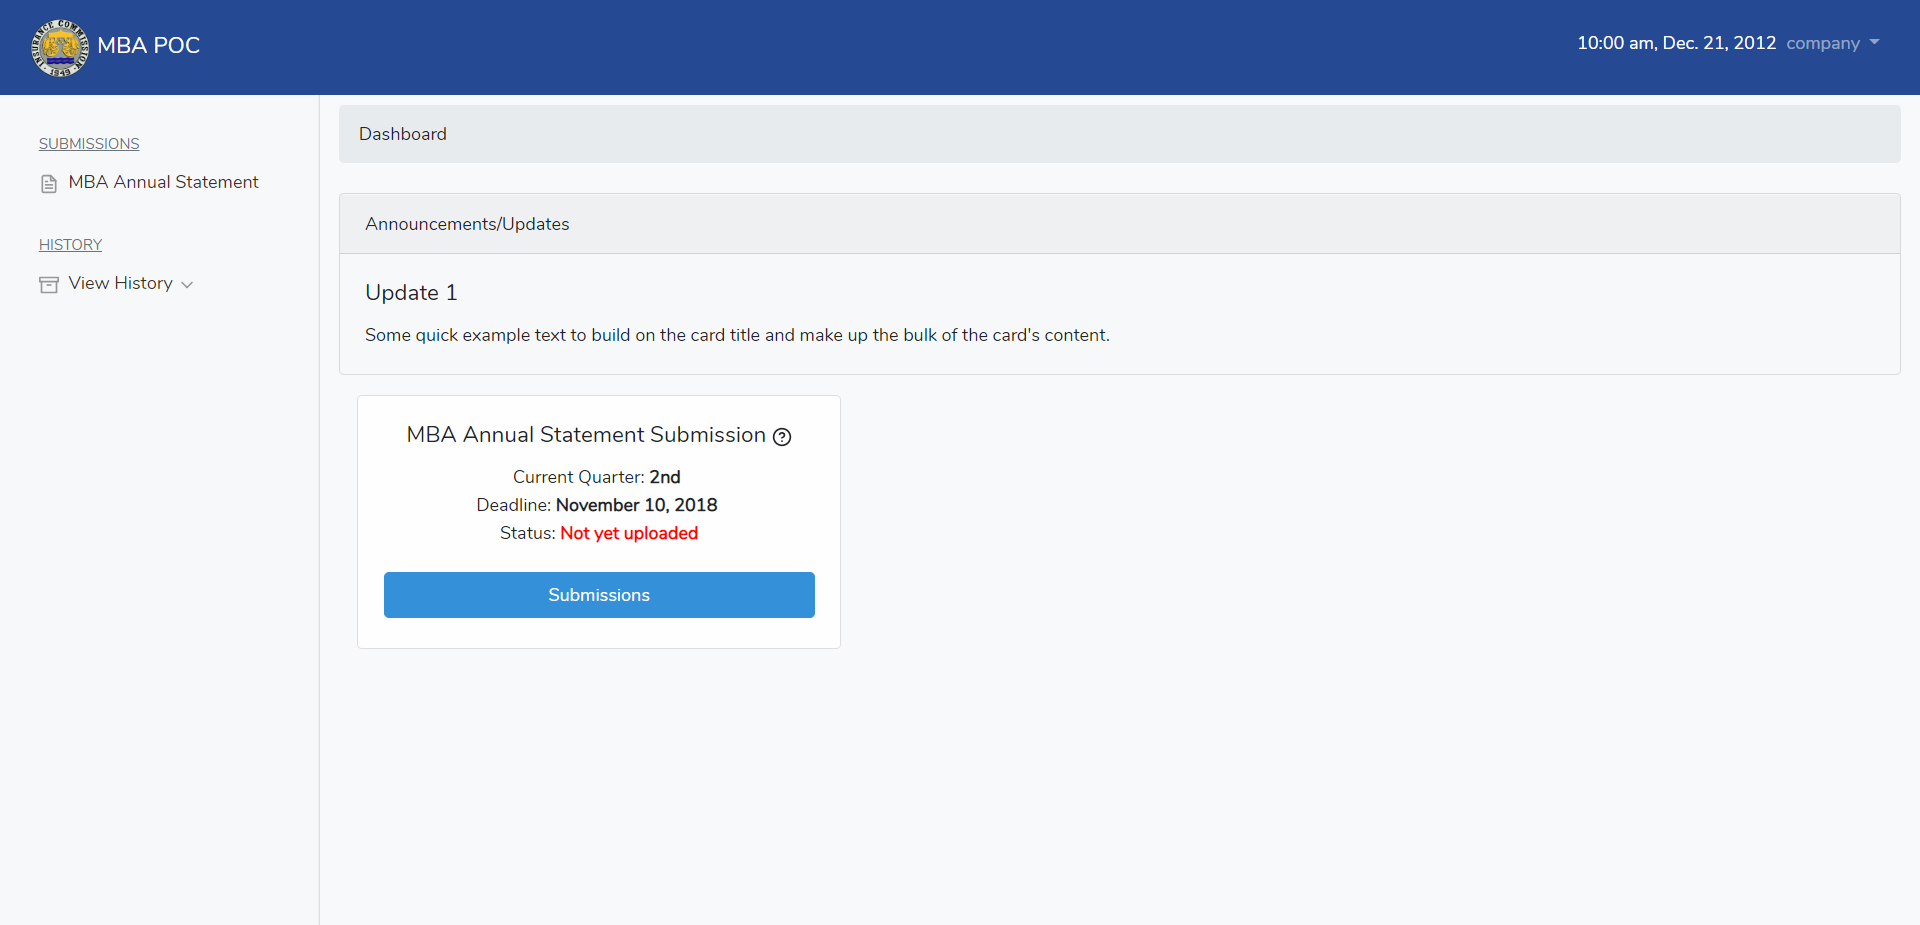
\includegraphics[keepaspectratio=true]{up-ic-screens/image22}{}\mdline{444}%mdk

%mdk-data-line={446}
\mdline{446}Upon clicking the Annual Submission card or the Annual
Statement from the sidebar, it will redirect to this page. Here, the
company can upload the required documents based on the checklist
provided by the insurance commission. Each file submission has specific
file type allowed. Once the required documents are passed, It will be
checked. The submit button is blocked out until all required documents
are uploaded. The company can also save as draft to continue uploading
later.%mdk

%mdk-data-line={455}
\mdhr{}%mdk

%mdk-data-line={457}
\noindent\mdline{457}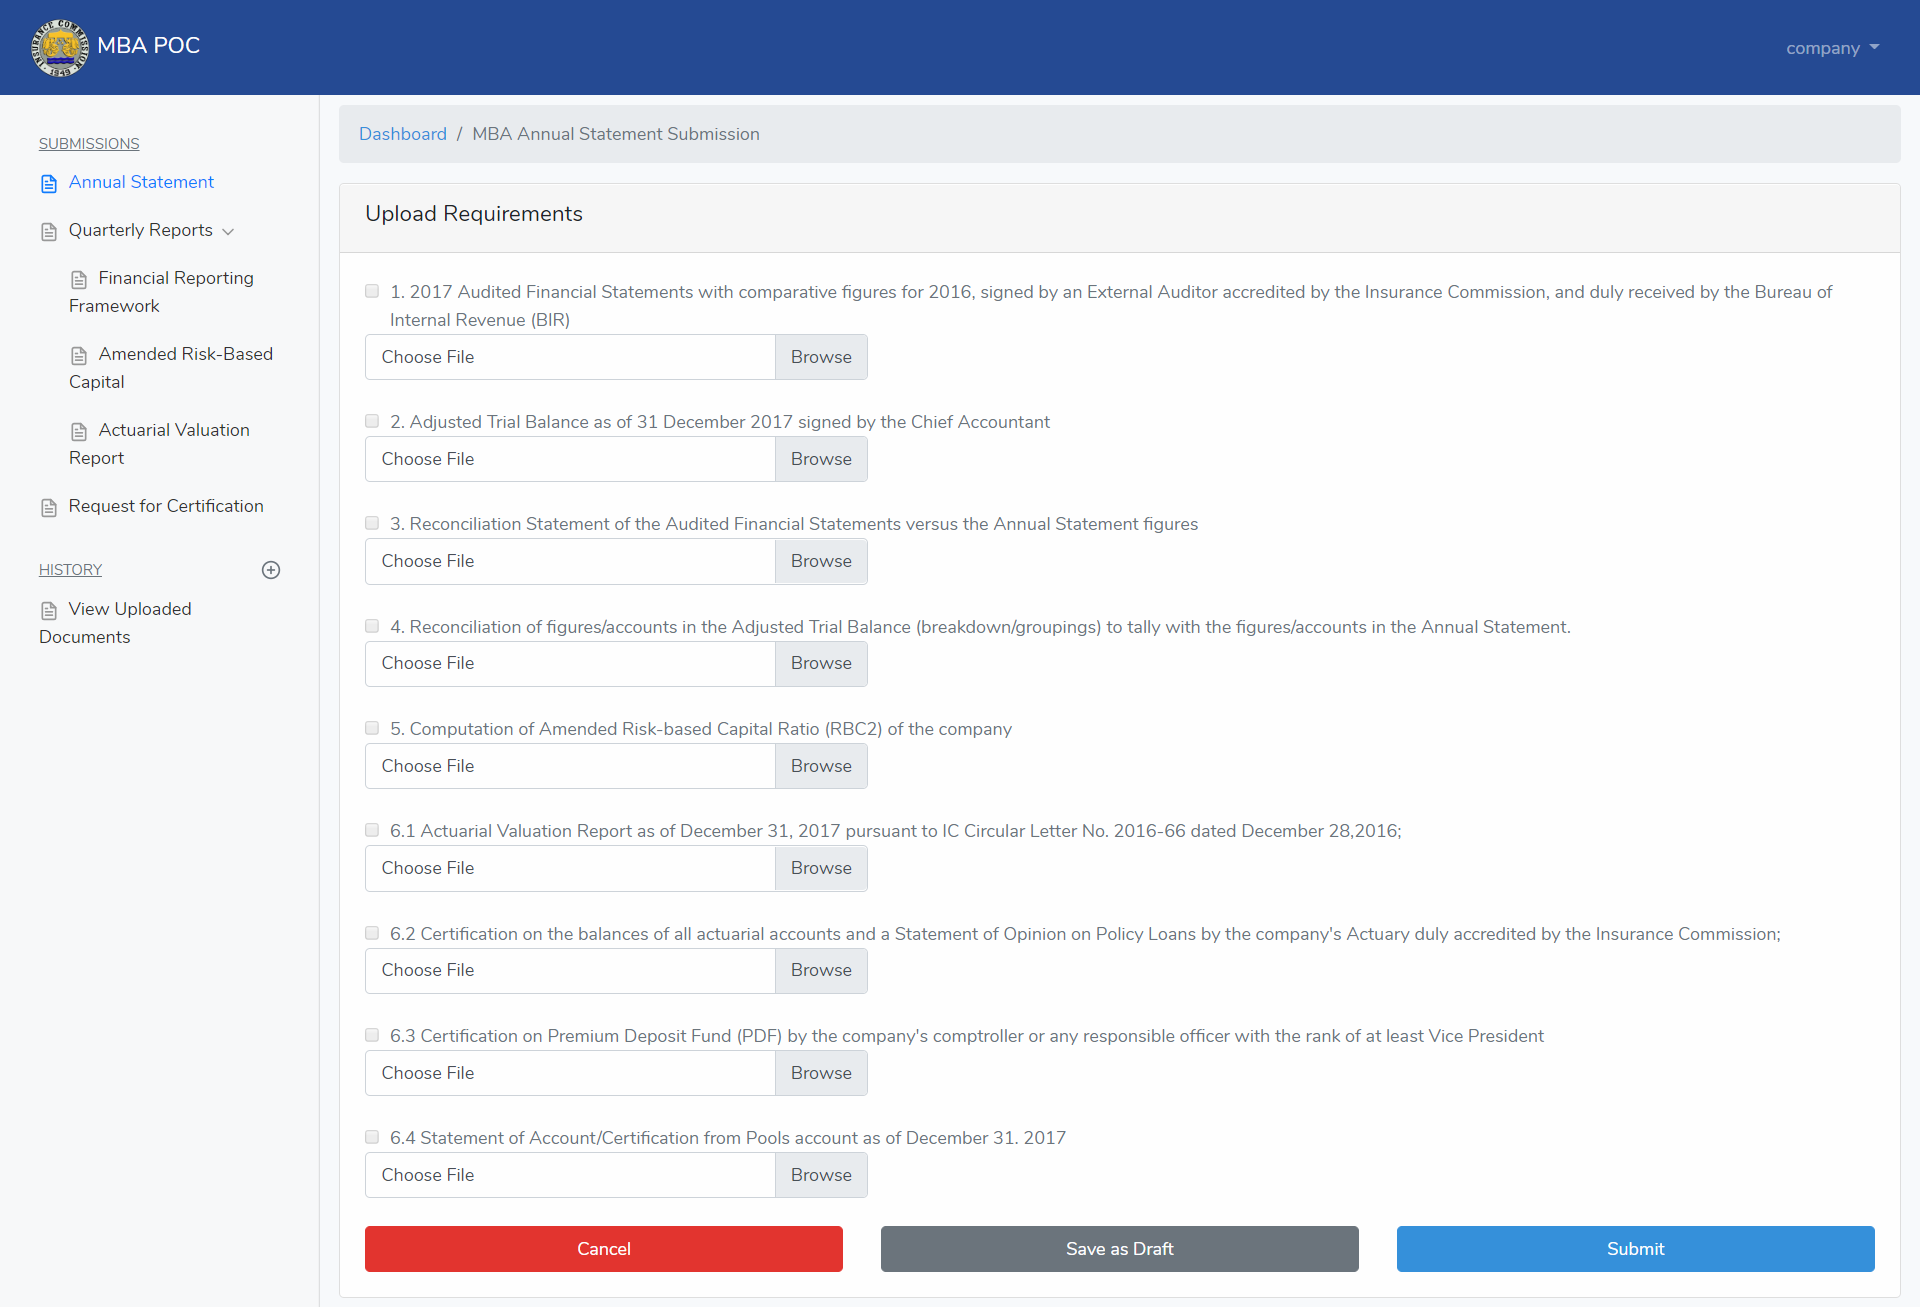
\includegraphics[keepaspectratio=true]{up-ic-screens/image206}{}\mdline{457}%mdk

%mdk-data-line={459}
\mdline{459}Upon clicking View History on the sidebar, the user is
given an option to which division submission it wants to view. In this
specific web screen, It can choose to view all its submissions to MBA
section. The main page has tables which are divided based on the
deadlines of each processes. Each tables can be sorted and filtered to
be able to track if they have submitted the documents.%mdk

%mdk-data-line={466}
\mdline{466}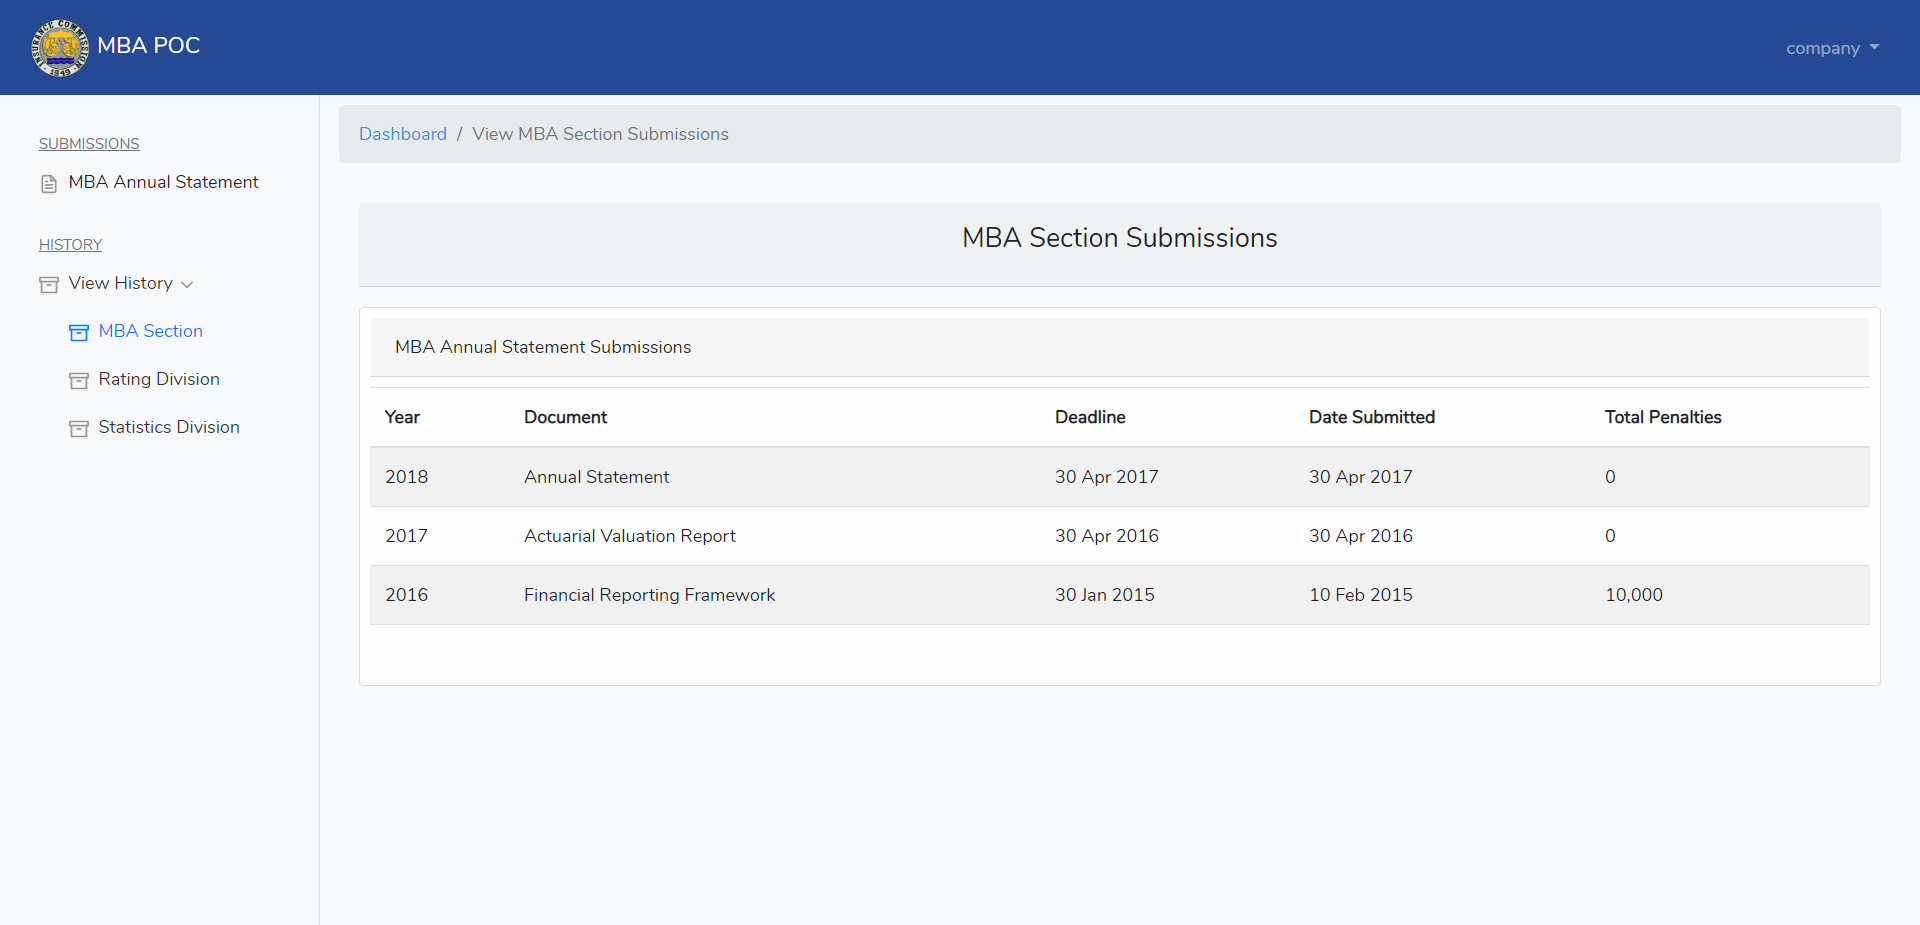
\includegraphics[keepaspectratio=true]{up-ic-screens/image10}{}\mdline{466}%mdk

%mdk-data-line={468}
\mdhr{}%mdk

%mdk-data-line={472}
\noindent\mdline{472}Examiner View%mdk

%mdk-data-line={474}
\mdline{474}This page will appear upon logging in an examiner account of
insurance commission. The page consist of a sidebar on the left side, a
navigation bar above with the insurance commission logo and a specified
label, if any. On the middle, it has the dashboard which has the cards
which are consisting of all the submissions needed to be done by the
companies. Each card consist of the Document submission header, current
quarter of submission and its deadline. Beside the document submission
header is a question icon which pops up a modal when clicked that
consist of requirements, guidelines and circular letters for that
specific submission. Below the page is a table of certificate requests.
The examiner can view incoming requests for certification of companies
through a table. The examiner can then take action on each request by
viewing it.\mdline{486}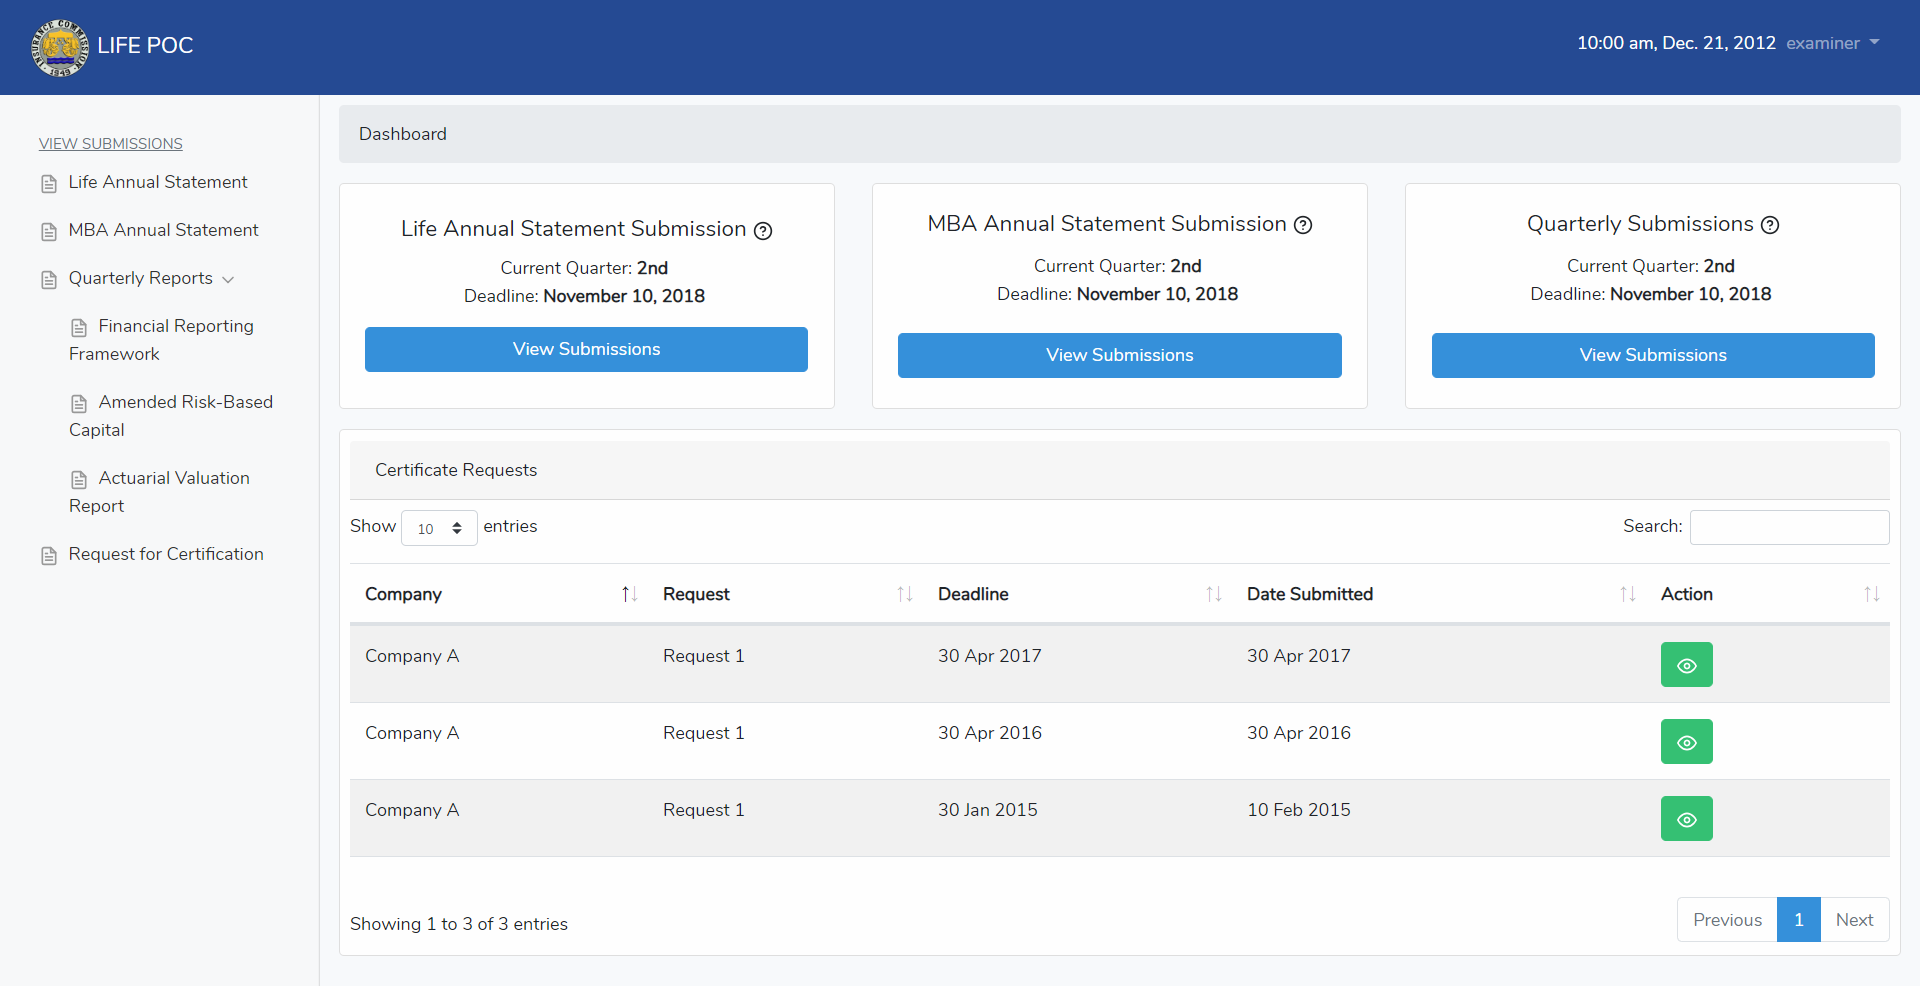
\includegraphics[keepaspectratio=true]{up-ic-screens/image47}{}\mdline{486}%mdk

%mdk-data-line={488}
\mdhr{}%mdk

%mdk-data-line={492}
\noindent\mdline{492}Upon clicking the MBA Annual Submission card or the MBA
Annual Statement from the sidebar, the examiner will be redirected to
the page with company list. The table with company list shows important
informations needed immediately for viewing. An examiner can also take
action of viewing the company submission in a much detailed form.%mdk

%mdk-data-line={498}
\mdline{498}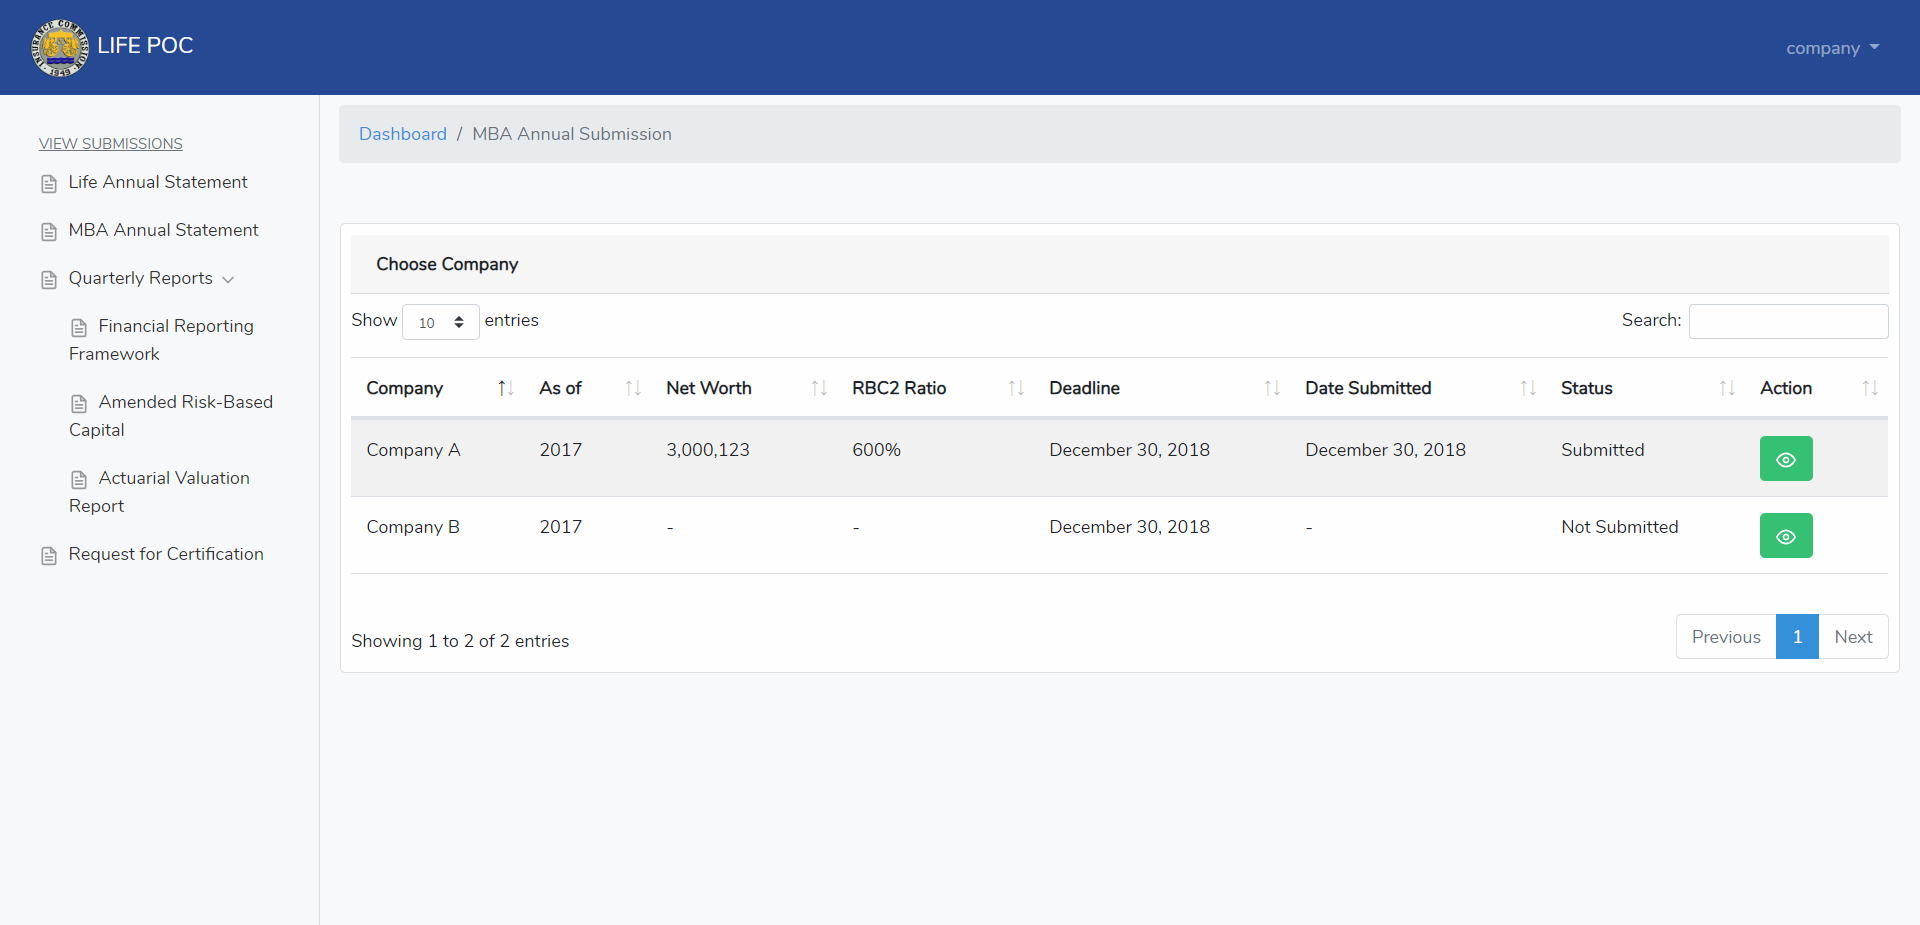
\includegraphics[keepaspectratio=true]{up-ic-screens/image120}{}\mdline{498}%mdk

%mdk-data-line={502}
\begin{enumerate}[noitemsep,topsep=\mdcompacttopsep]%mdk

%mdk-data-line={502}
\item{}
%mdk-data-line={502}
\subsubsection{\mdline{502}2.3.3.\hspace*{0.5em}\mdline{502}Quarterly Submission and Examination of FRF, RBC2, and Actuarial Valuation Report}\label{sec-quarterly-submission-and-examination-of-frf-rbc2-and-actuarial-valuation-report}%mdk%mdk%mdk
%mdk
\end{enumerate}%mdk

%mdk-data-line={506}
\noindent\mdline{506}Company View%mdk

%mdk-data-line={508}
\mdline{508}This page will appear upon logging in a company
account. The page consist of a sidebar on the left side, a navigation
bar above with the insurance commission logo and a specified label, if
any. On the middle, it has the dashboard which has the
announcements/updates regarding submissions of documents. There\mdline{512}'\mdline{512}s also
the cards which are consisting of all the submissions needed by the
companies. Each card consist of the Document submission header, current
quarter of submission, its deadline and status of the company on
submission. Beside the document submission header is a question icon
which pops up a modal when clicked that consist of requirements,
guidelines and circular letters for that specific submission.%mdk

%mdk-data-line={520}
\mdline{520}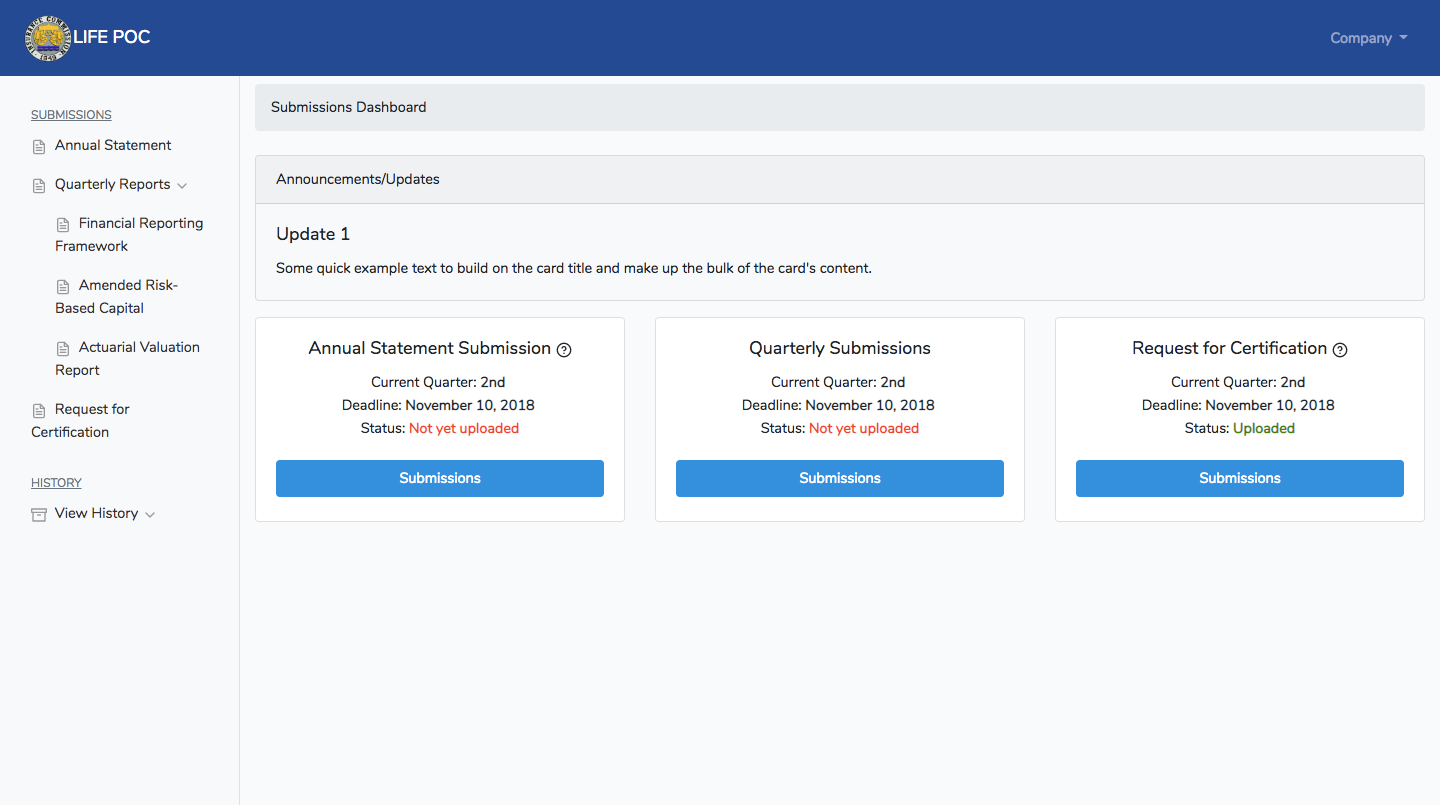
\includegraphics[keepaspectratio=true]{up-ic-screens/image148}{}\mdline{520}%mdk

%mdk-data-line={522}
\mdhr{}%mdk

%mdk-data-line={526}
\noindent\mdline{526}Upon clicking the Quarterly Submission on the sidebar
or the button on the Quarterly Submission card, it will redirect to this
page. This page lists down further processes on quarterly submission.
From each quarterly document submission, the user has the option to
upload file or input forms.%mdk

%mdk-data-line={532}
\mdline{532}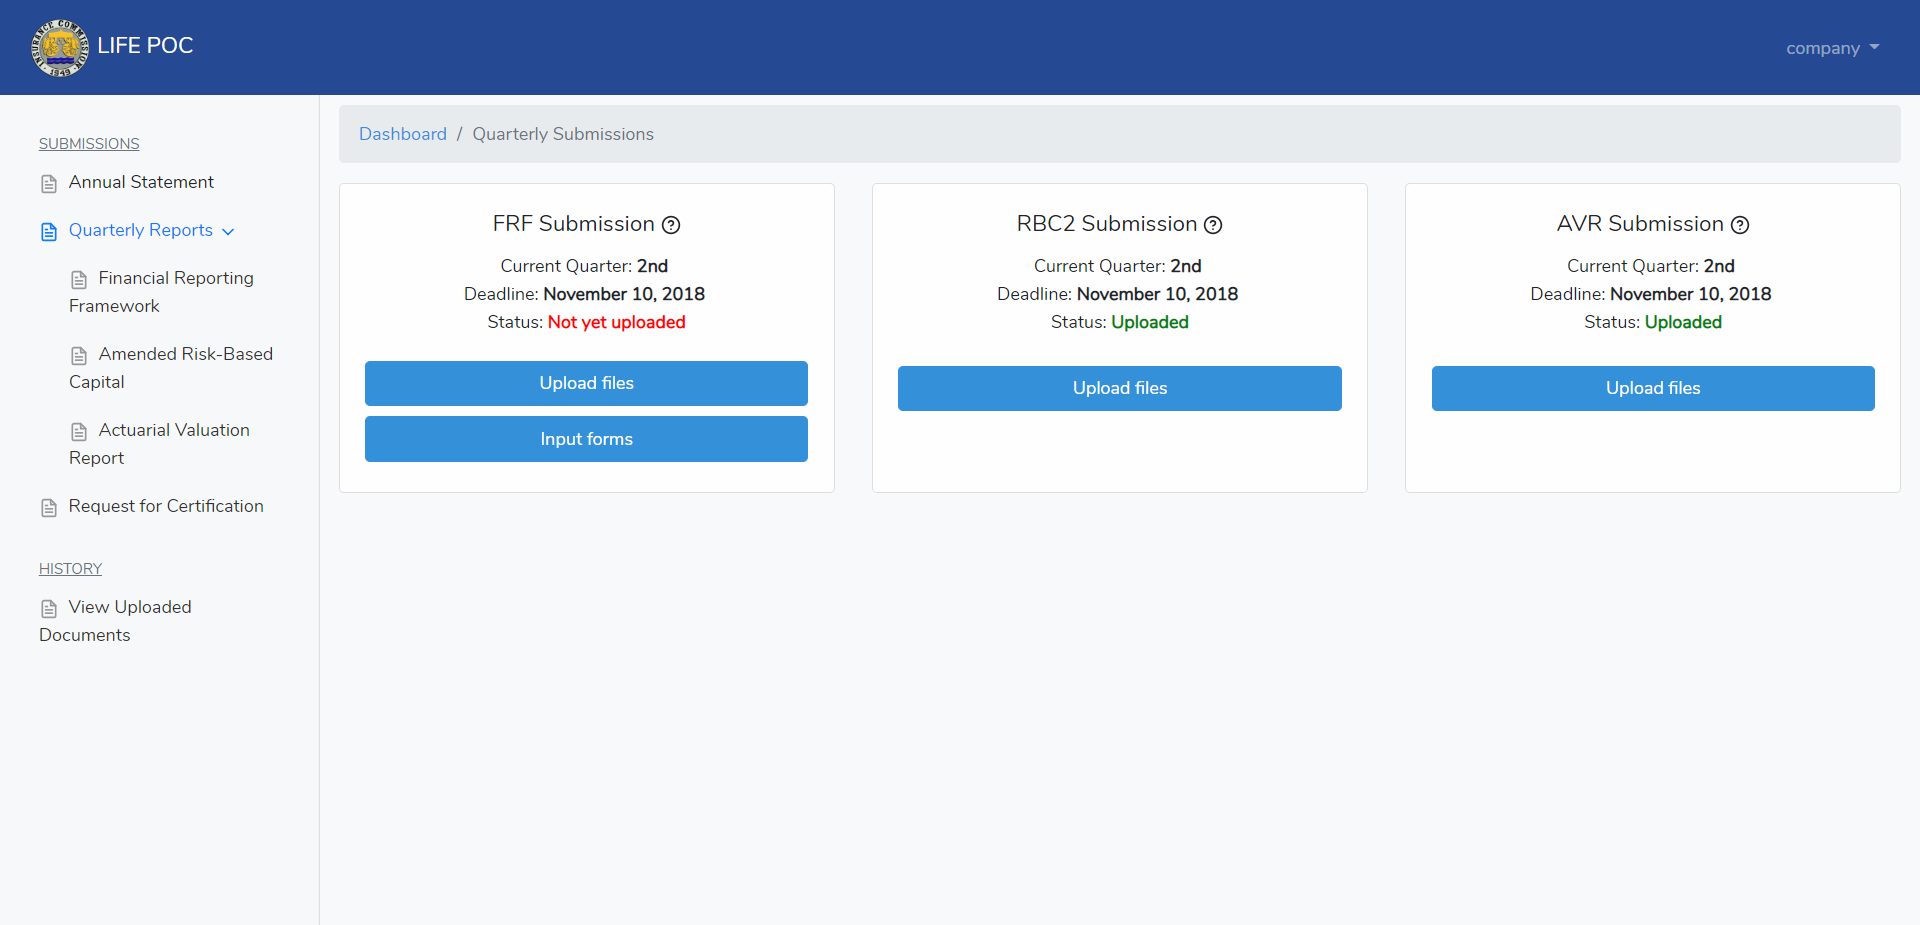
\includegraphics[keepaspectratio=true]{up-ic-screens/image36}{}\mdline{532}%mdk

%mdk-data-line={534}
\mdhr{}%mdk

%mdk-data-line={538}
\noindent\mdline{538}Upon clicking inputs forms from the quarterly submissions page for
FRF, it will redirect to this page. The company can input their account
here just like what they would in an excel sheet.%mdk

%mdk-data-line={542}
\mdline{542}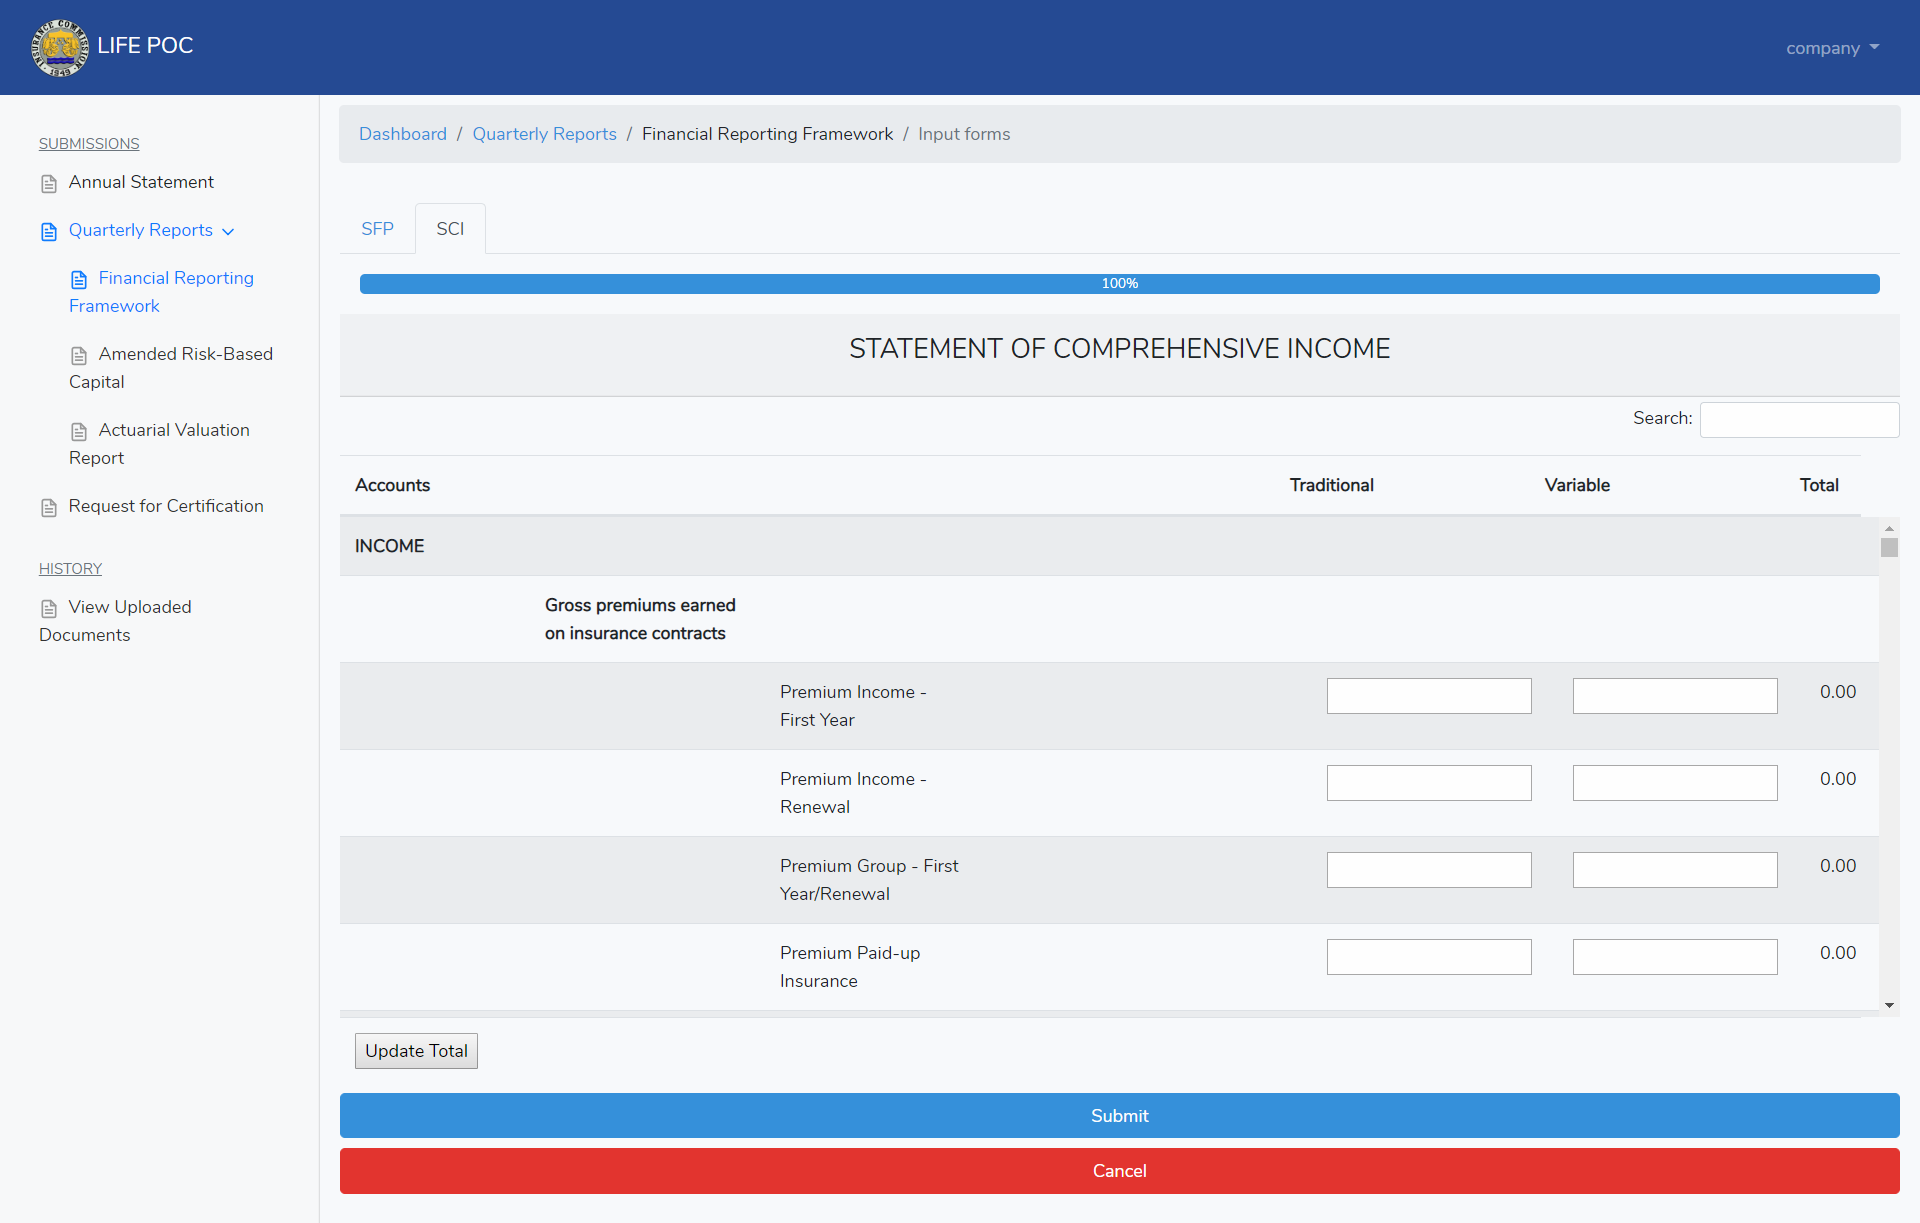
\includegraphics[keepaspectratio=true]{up-ic-screens/image166}{}\mdline{542}%mdk

%mdk-data-line={544}
\mdhr{}%mdk

%mdk-data-line={548}
\noindent\mdline{548}Upon clicking upload file from the quarterly
submissions page for FRF, it will redirect to this page. The user can
upload the specified template for the FRF submission. It shall follow
the naming convention as well as the file type specified (excel) to be
able to upload.%mdk

%mdk-data-line={554}
\mdline{554}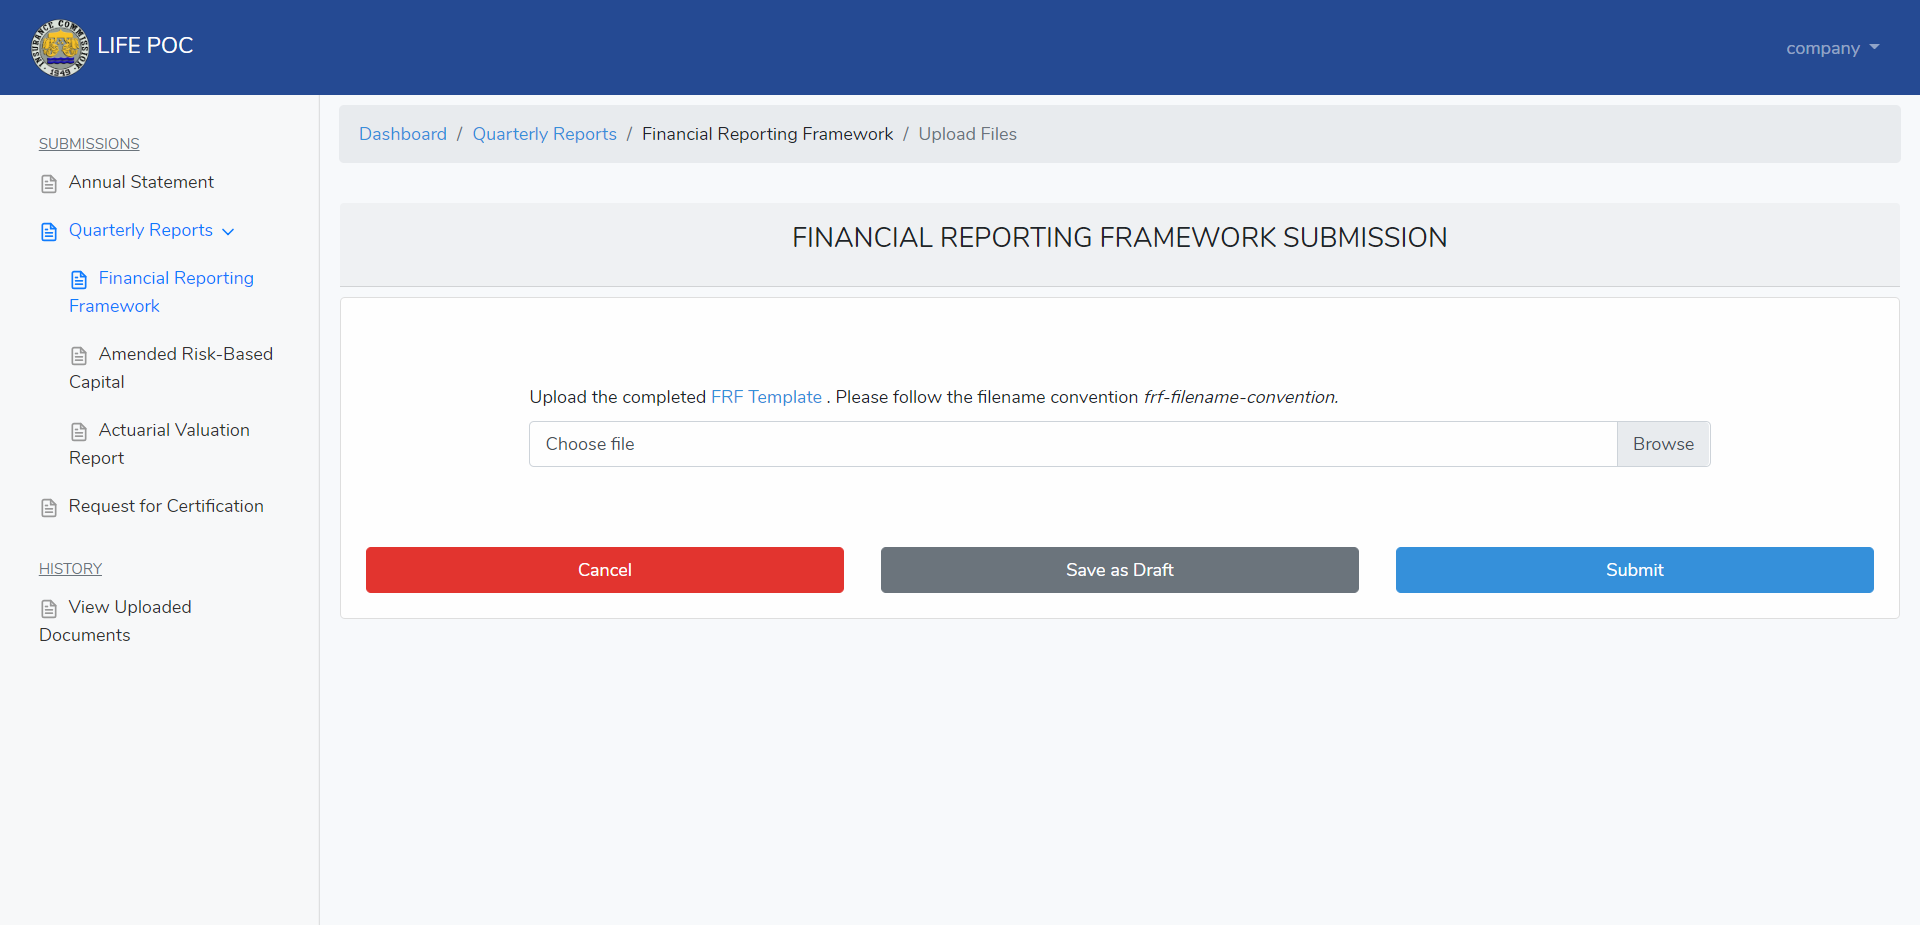
\includegraphics[keepaspectratio=true]{up-ic-screens/image29}{}\mdline{554}%mdk

%mdk-data-line={556}
\mdline{556}Upon clicking upload file from the quarterly
submissions page for RBC2, it will redirect to this page. The user can
upload the specified template for the RBC2 submission. It shall follow
the naming convention as well as the file type specified (excel) to be
able to upload.%mdk

%mdk-data-line={562}
\mdline{562}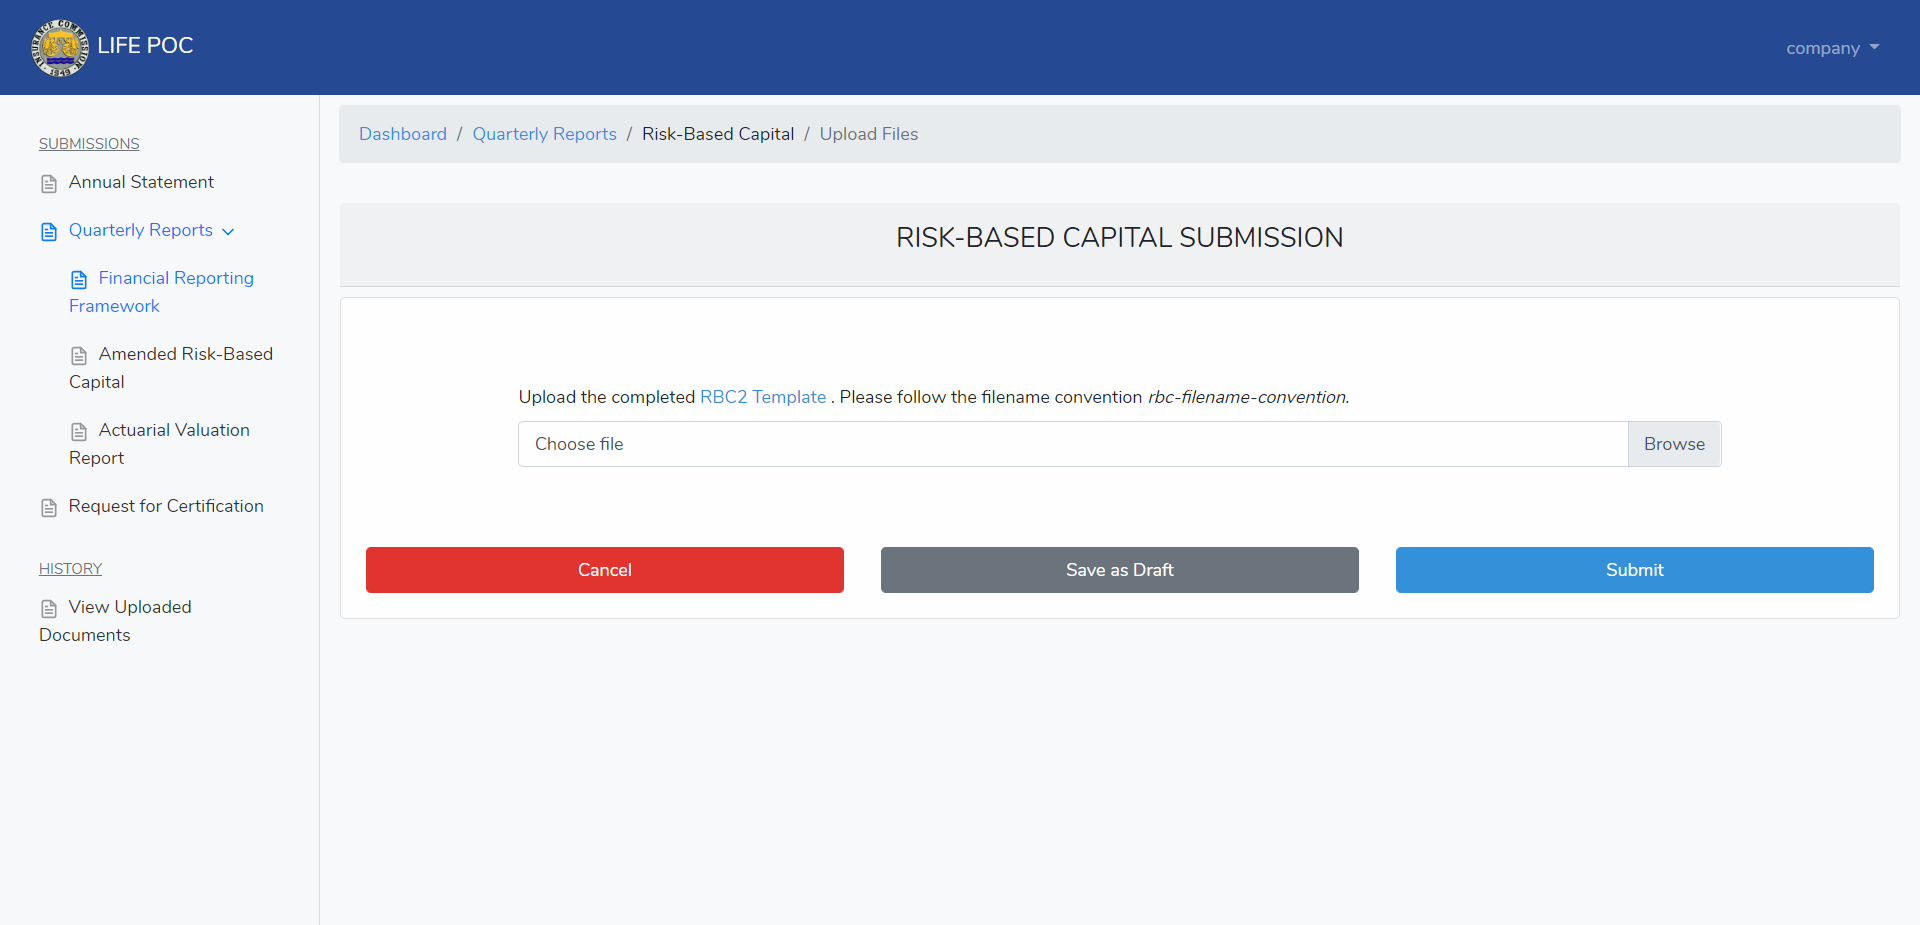
\includegraphics[keepaspectratio=true]{up-ic-screens/image85}{}\mdline{562}%mdk

%mdk-data-line={564}
\mdline{564}Upon clicking upload file from the quarterly
submissions page for AVR, it will redirect to this page. The user can
upload the specified template for the AVR submission. It shall follow
the naming convention as well as the file type specified (excel) to be
able to upload.%mdk

%mdk-data-line={570}
\mdline{570}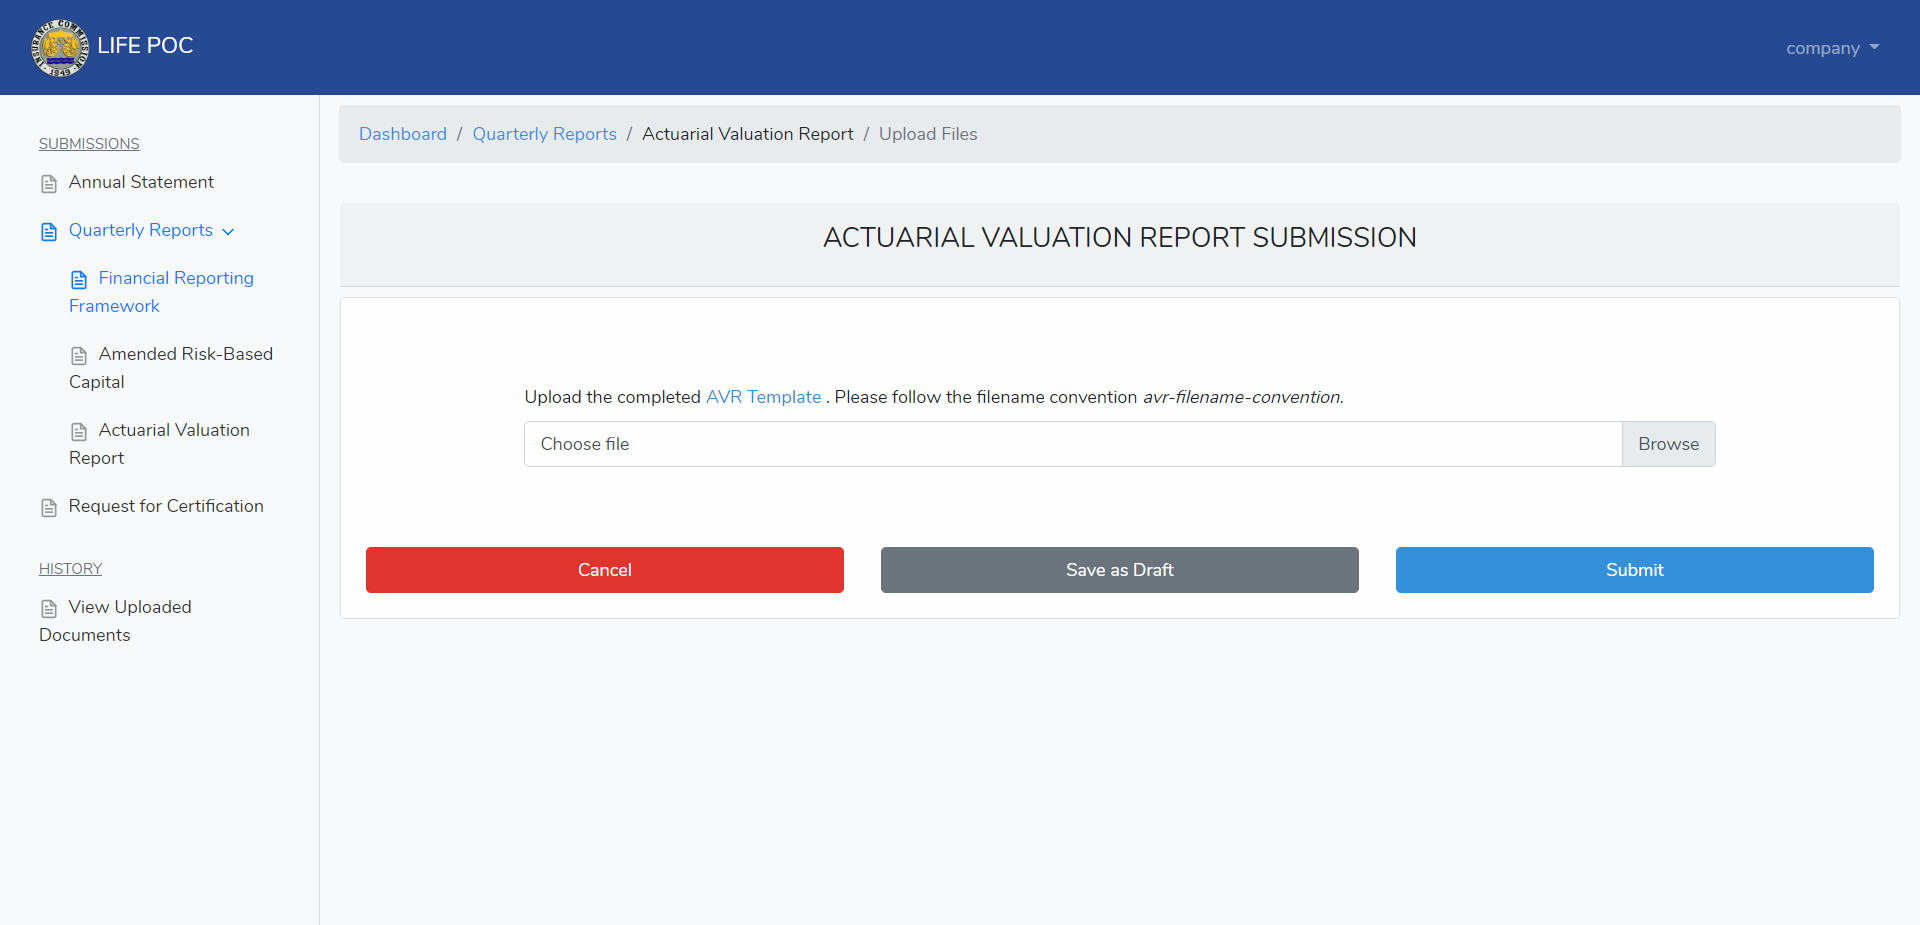
\includegraphics[keepaspectratio=true]{up-ic-screens/image126}{}\mdline{570}%mdk

%mdk-data-line={572}
\mdhr{}%mdk

%mdk-data-line={576}
\noindent\mdline{576}Upon clicking View History on the sidebar, the user is
given an option to which division submission it wants to view. In this
specific web screen, It can choose to view all its submissions to Life
division. The main page has tables which are divided based on the
deadlines of each processes. Each tables can be sorted and filtered to
be able to track if they have submitted the documents.%mdk

%mdk-data-line={583}
\mdline{583}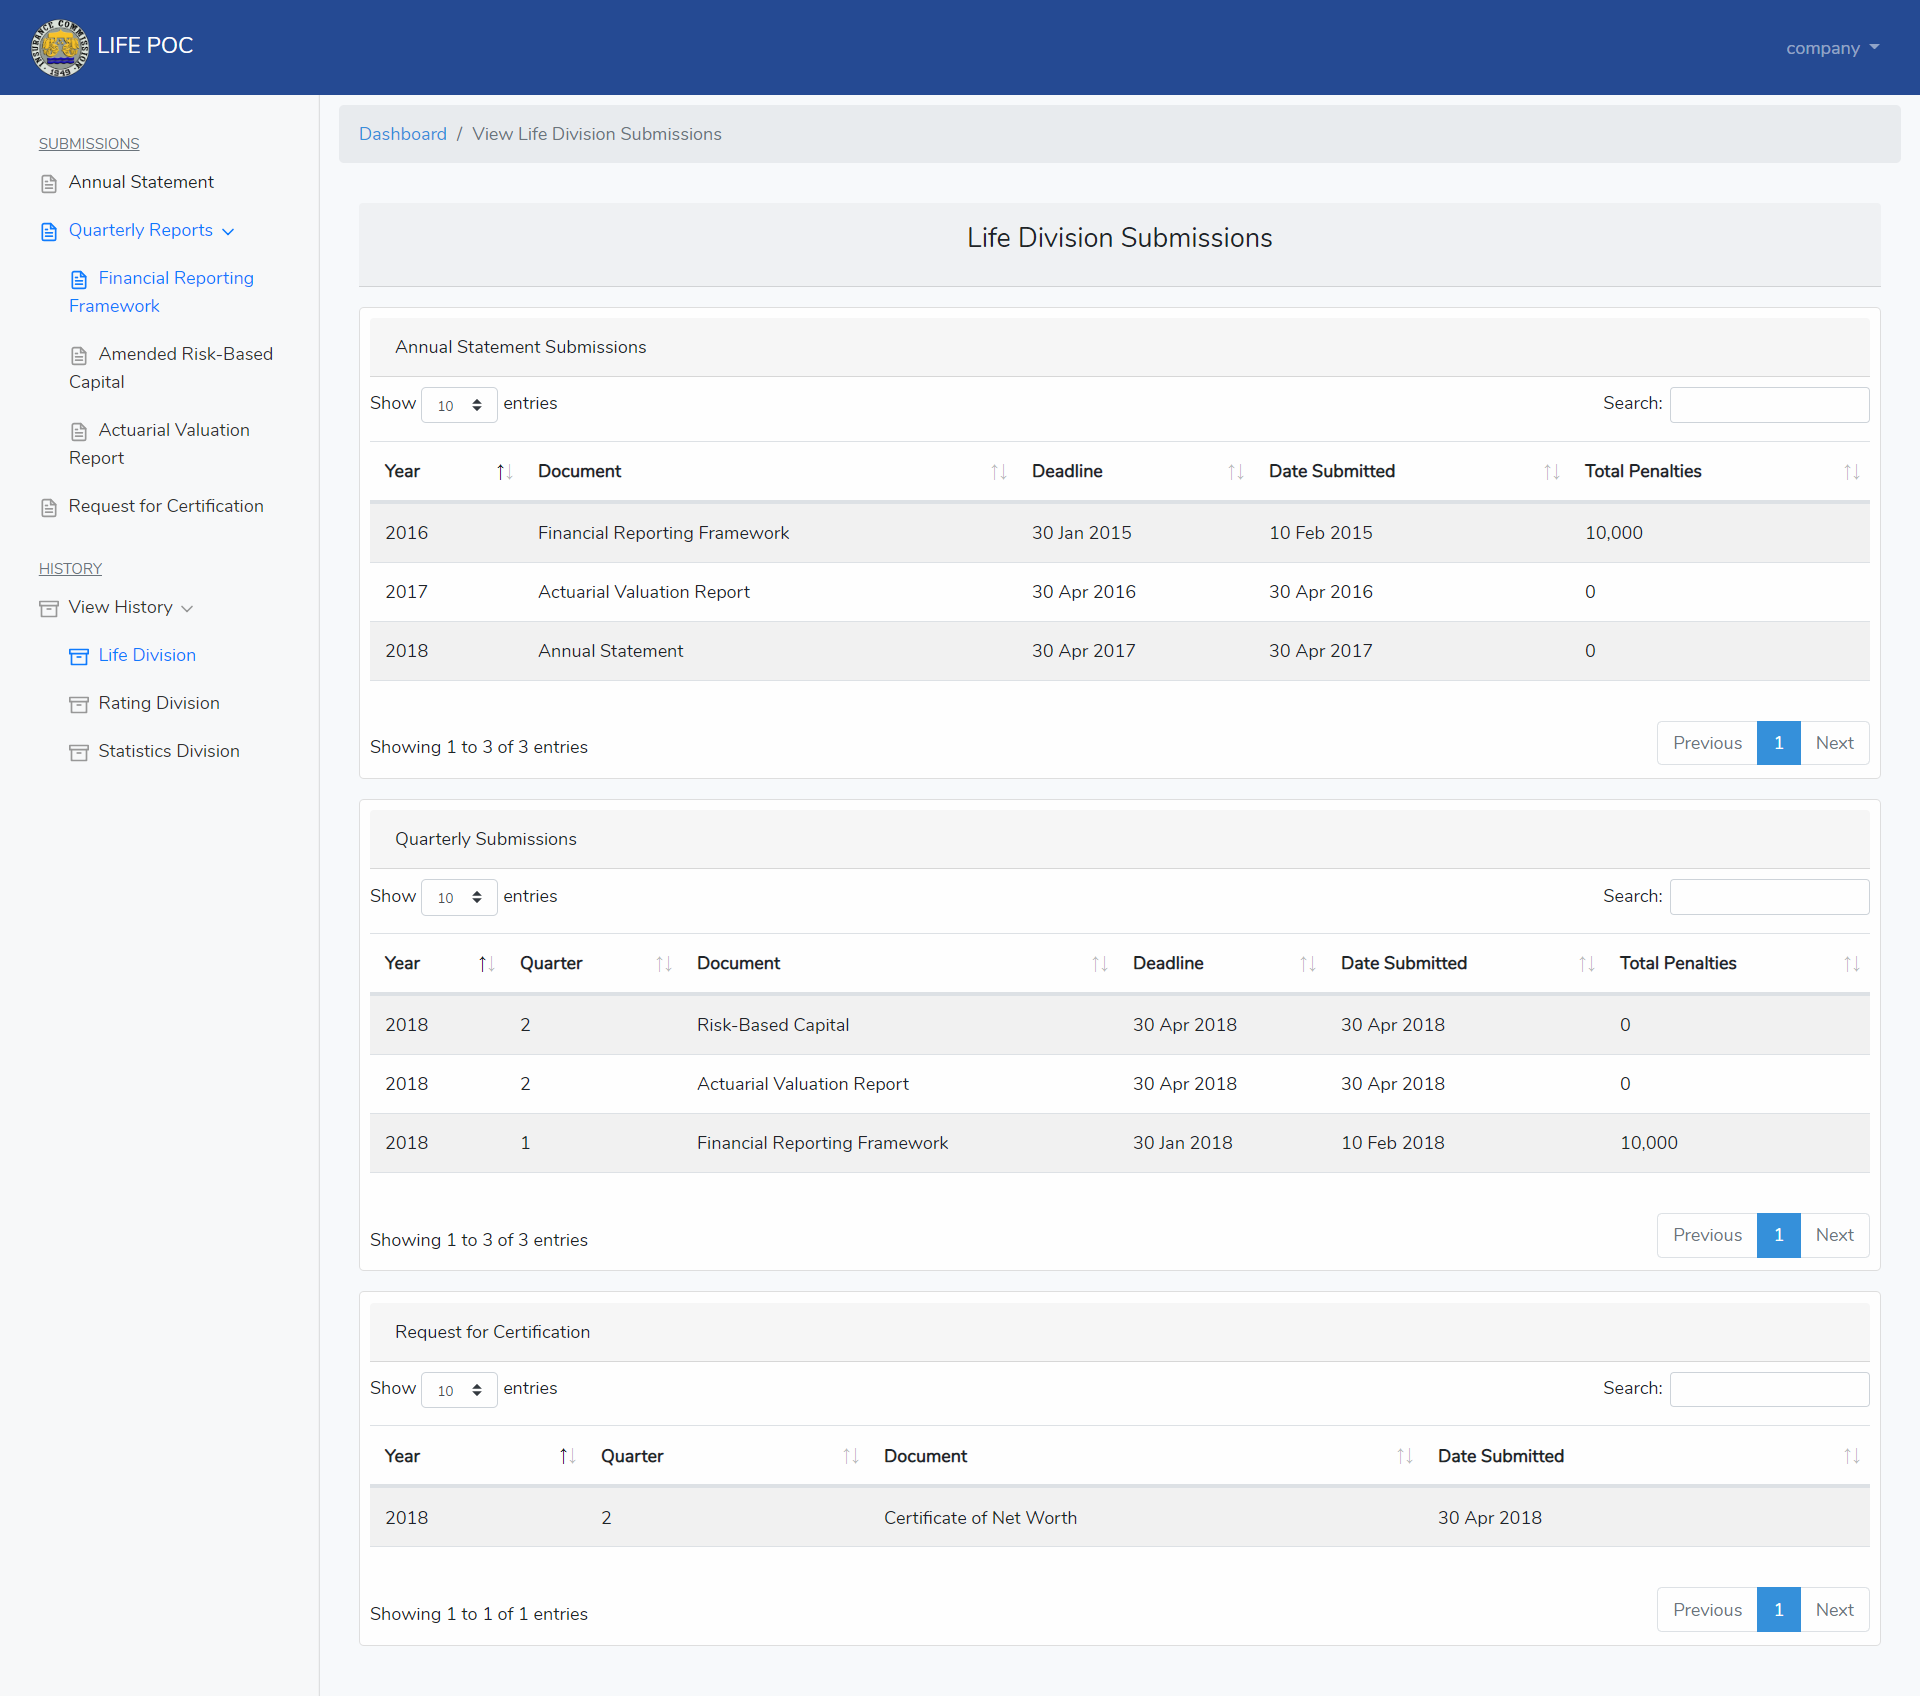
\includegraphics[keepaspectratio=true]{up-ic-screens/image99}{}\mdline{583}%mdk

%mdk-data-line={585}
\mdhr{}%mdk

%mdk-data-line={589}
\noindent\mdline{589}Examiner View%mdk

%mdk-data-line={591}
\mdline{591}This page will appear upon logging in an examiner
account of insurance commission. The page consist of a sidebar on the
left side, a navigation bar above with the insurance commission logo and
a specified label, if any. On the middle, it has the dashboard which has
the cards which are consisting of all the submissions needed to be done
by the companies. Each card consist of the Document submission header,
current quarter of submission and its deadline. Beside the document
submission header is a question icon which pops up a modal when clicked
that consist of requirements, guidelines and circular letters for that
specific submission. Below the page is a table of certificate requests.
The examiner can view incoming requests for certification of companies
through a table. The examiner can then take action on each request by
viewing it.%mdk

%mdk-data-line={605}
\mdline{605}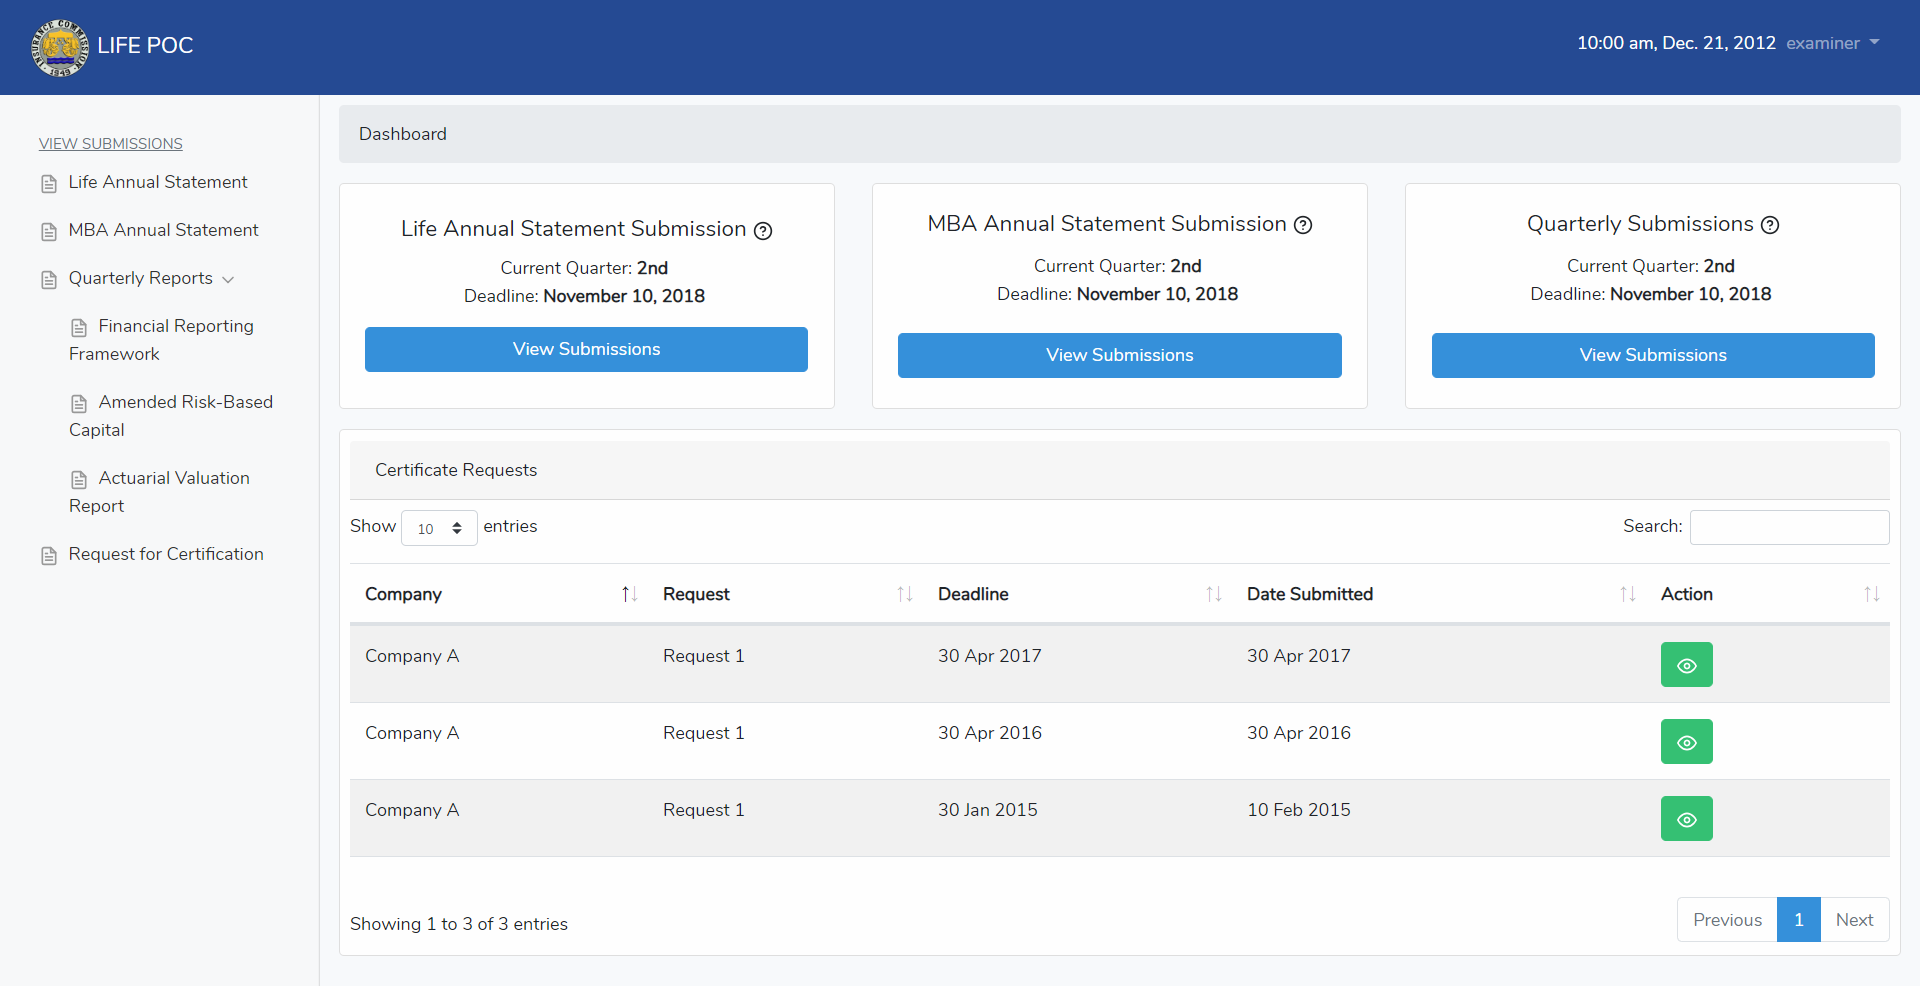
\includegraphics[keepaspectratio=true]{up-ic-screens/image47}{}\mdline{605}%mdk

%mdk-data-line={607}
\mdhr{}%mdk

%mdk-data-line={611}
\noindent\mdline{611}Upon clicking the Quarterly Submission button from the
card or the Quarterly Submission from the sidebar, the examiner will be
redirected to this page. This page lists down further processes on
quarterly submission. From each quarterly document submission, the
examiner has the option to view company submissions by clicking View
submissions.%mdk

%mdk-data-line={618}
\mdline{618}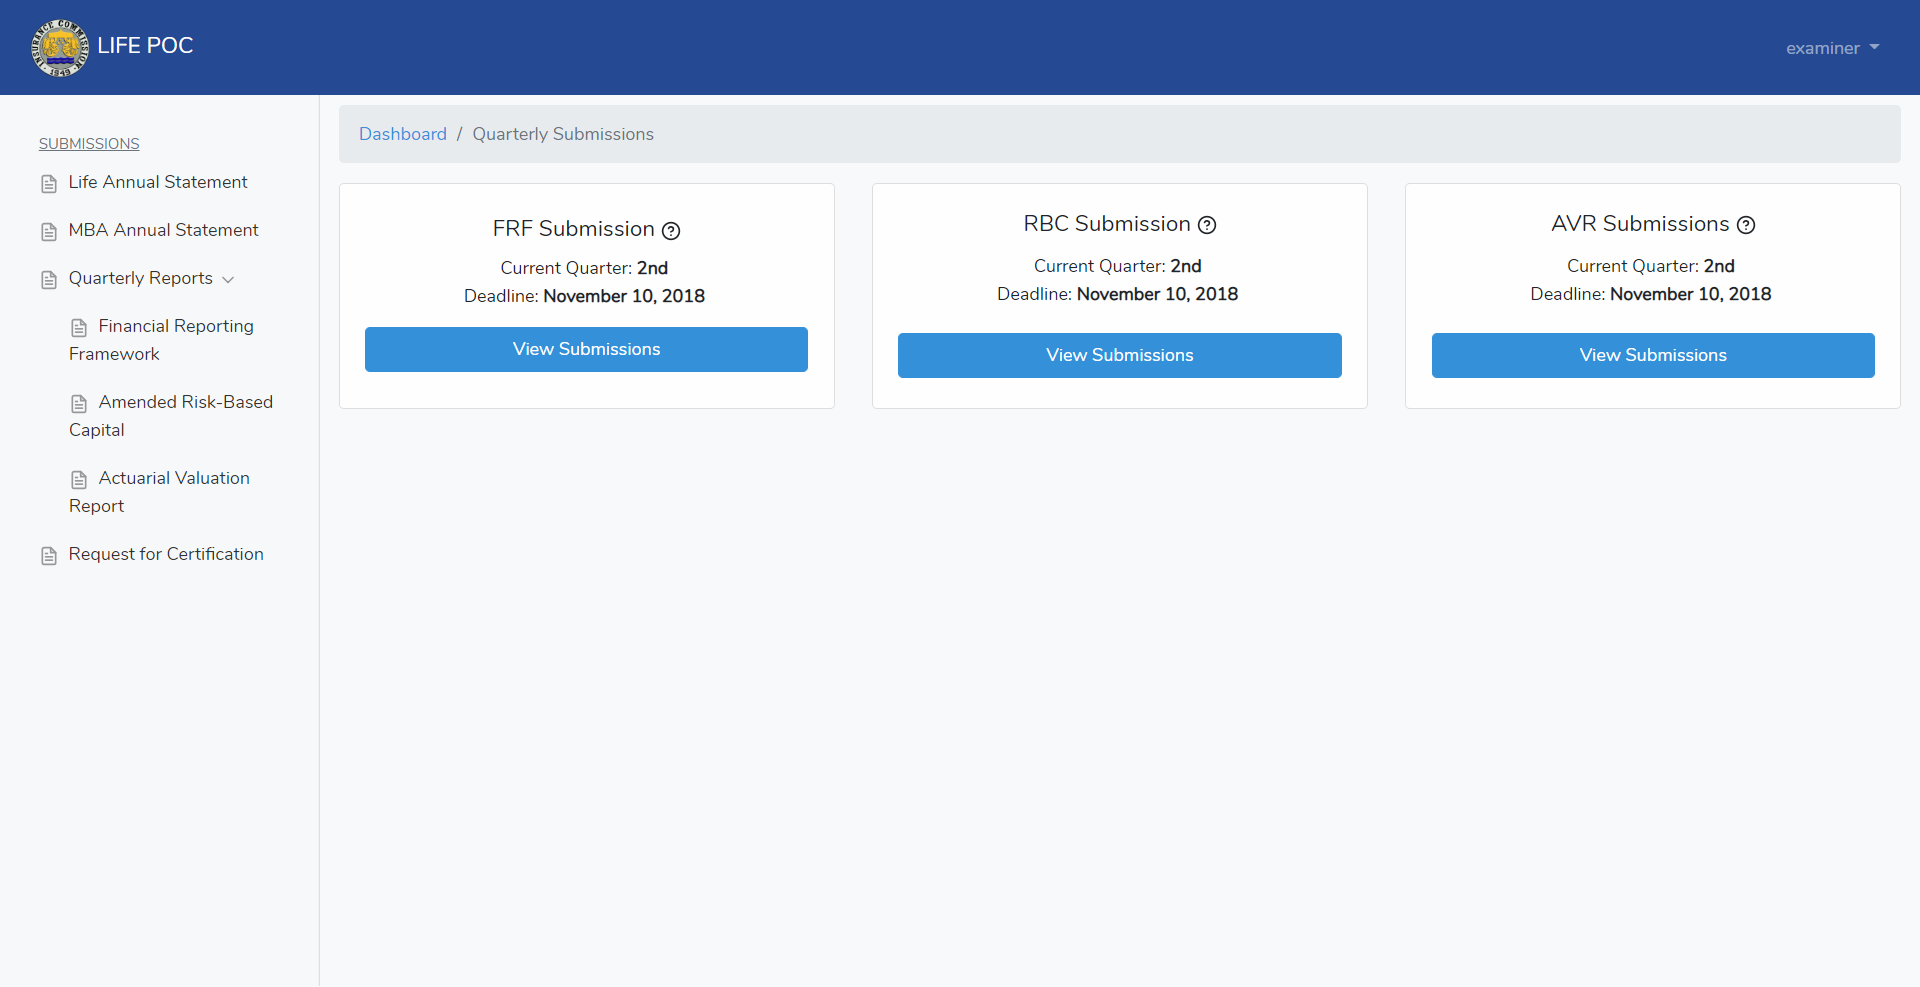
\includegraphics[keepaspectratio=true]{up-ic-screens/image1}{}\mdline{618}%mdk

%mdk-data-line={620}
\mdhr{}%mdk

%mdk-data-line={624}
\noindent\mdline{624}Upon clicking the View Submissions from the FRF
Submissions card on Quarterly Submissions page, the examiner will be
redirected to the page with company list. The table with company list
shows important informations needed immediately for viewing. An examiner
can also take action of viewing the company submission in a much
detailed form.%mdk

%mdk-data-line={631}
\mdline{631}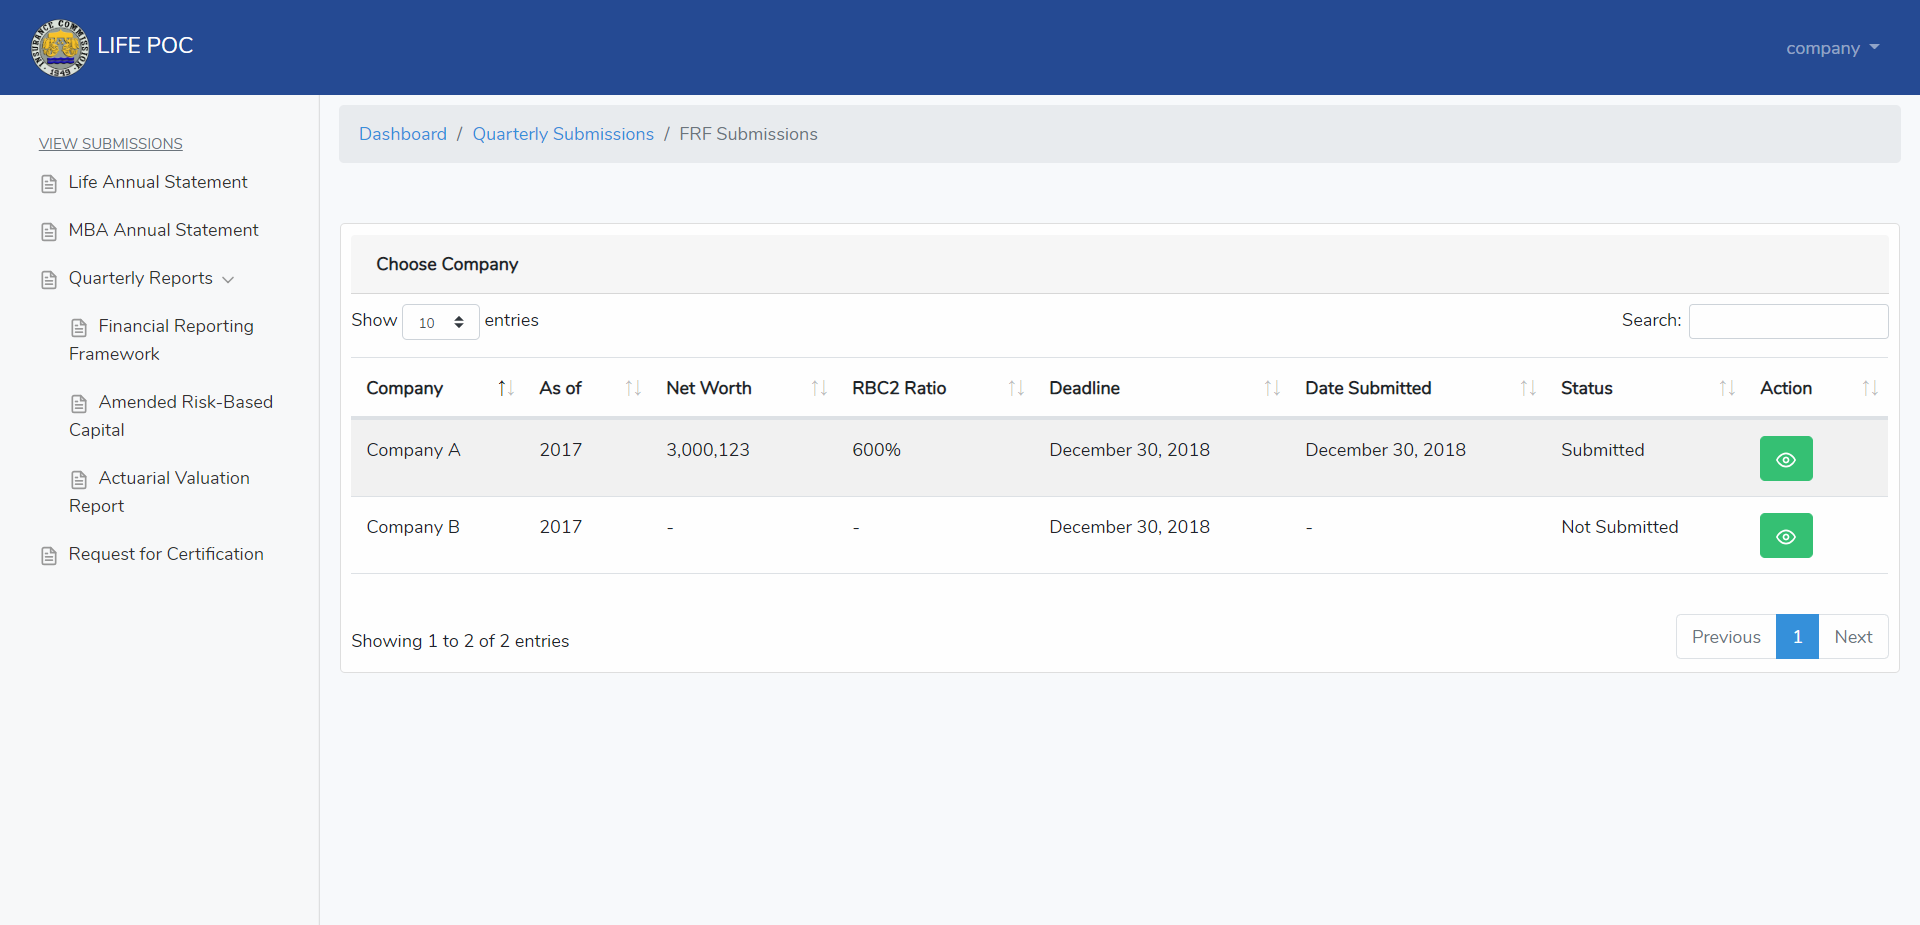
\includegraphics[keepaspectratio=true]{up-ic-screens/image97}{}\mdline{631}%mdk

%mdk-data-line={637}
\mdhr{}%mdk

%mdk-data-line={641}
\noindent\mdline{641}Upon clicking the View Submissions from the RBC
Submissions card on Quarterly Submissions page, the examiner will be
redirected to the page with company list. The table with company list
shows important informations needed immediately for viewing. An examiner
can also take action of viewing the company submission in a much
detailed form.%mdk

%mdk-data-line={648}
\mdline{648}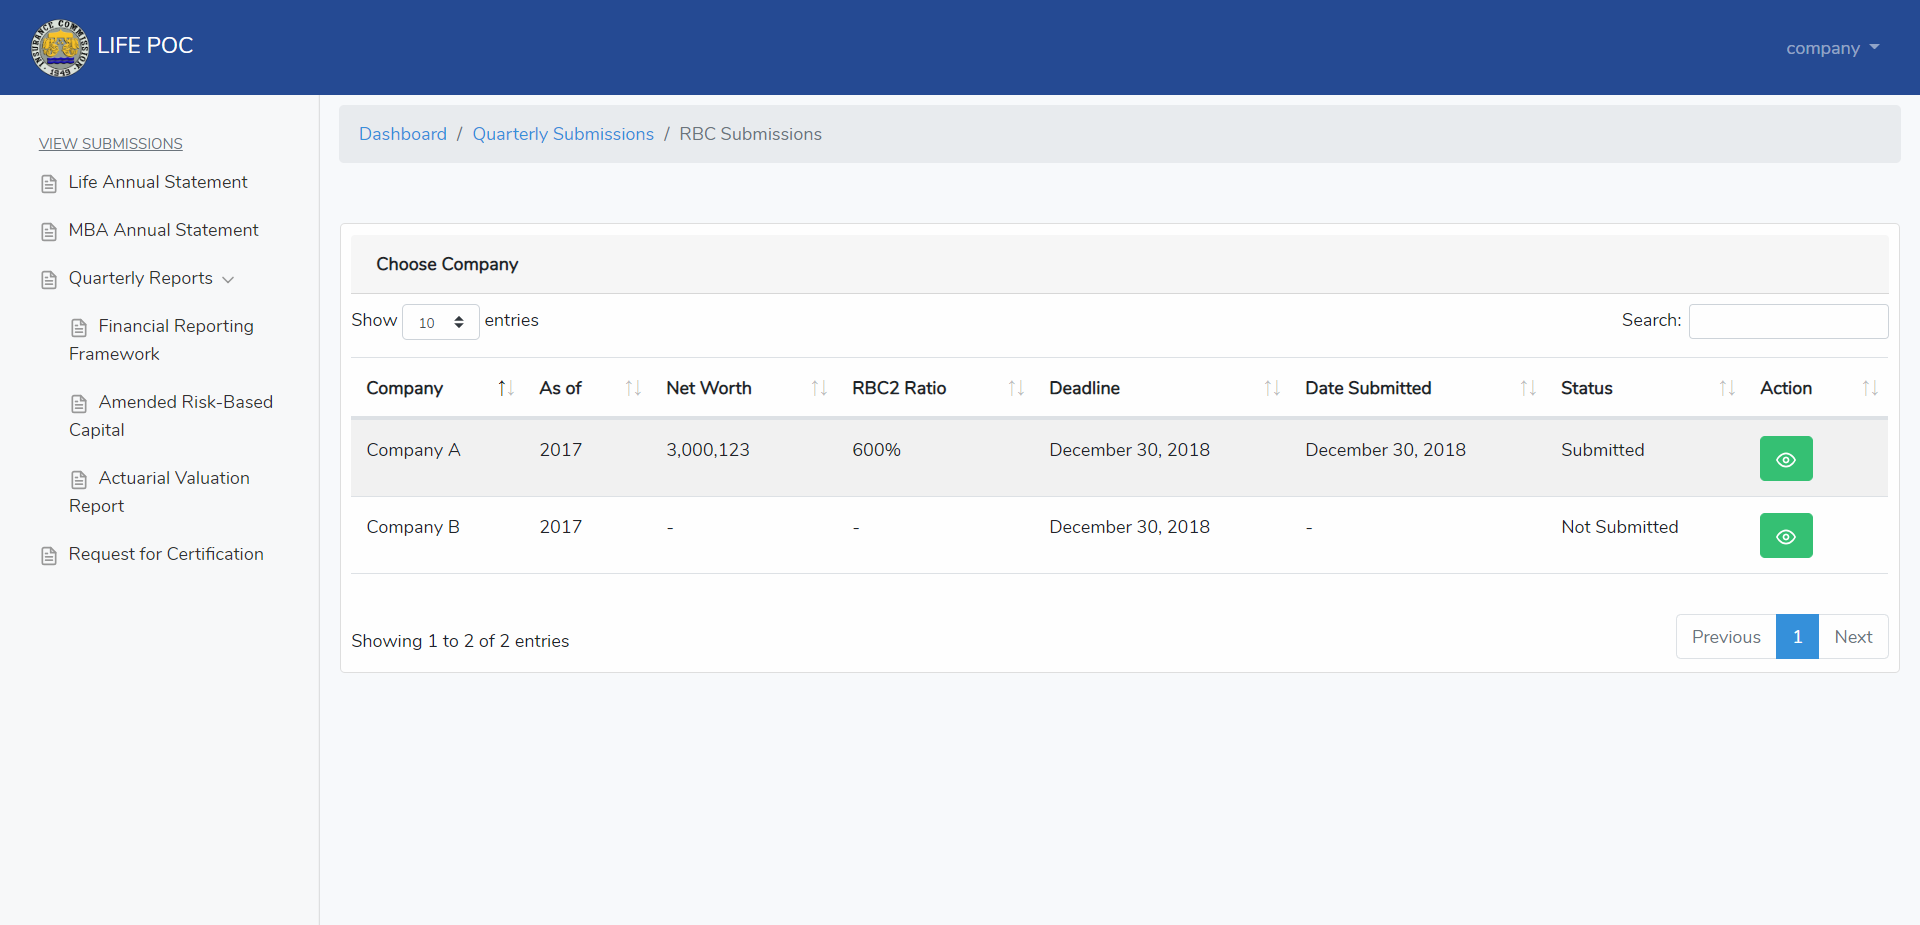
\includegraphics[keepaspectratio=true]{up-ic-screens/image106}{}\mdline{648}%mdk

%mdk-data-line={670}
\mdline{670}Upon clicking the view button, it will redirect to this
page where you can change the status, download submitted checklist, and
company files.%mdk

%mdk-data-line={674}
\mdline{674}\includegraphics[keepaspectratio=true]{up-ic-screens/image198}{}\mdline{674}%mdk

%mdk-data-line={676}
\mdline{676}Note: Show the computation for RBC%mdk

%mdk-data-line={694}
\mdline{694}Upon clicking the View Submissions from the AVR
Submissions card on Quarterly Submissions page, the examiner will be
redirected to the page with company list. The table with company list
shows important informations needed immediately for viewing. An examiner
can also take action of viewing the company submission in a much
detailed form.%mdk

%mdk-data-line={701}
\mdline{701}\includegraphics[keepaspectratio=true]{up-ic-screens/image177}{}\mdline{701}%mdk

%mdk-data-line={705}
\mdhr{}%mdk

%mdk-data-line={708}
\noindent\mdline{708}=============================%mdk

%mdk-data-line={710}
\subsection{\mdline{710}2.4.\hspace*{0.5em}\mdline{710}1.  Non-Life Division}\label{sec-1-non-life-division}%mdk%mdk

%mdk-data-line={715}
\begin{enumerate}[noitemsep,topsep=\mdcompacttopsep]%mdk

%mdk-data-line={715}
\item{}
%mdk-data-line={715}
\subsubsection{\mdline{715}2.4.1.\hspace*{0.5em}\mdline{715}Annual Submission and Examination of Financial Standing of Non-Life Companies}\label{sec-annual-submission-and-examination-of-financial-standing-of-non-life-companies}%mdk%mdk%mdk
%mdk
\end{enumerate}%mdk

%mdk-data-line={717}
\noindent\mdline{717}\includegraphics[keepaspectratio=true]{up-ic-screens/image89}{}\mdline{717}%mdk

%mdk-data-line={719}
\mdline{719}{}[\mdline{719}Company Side\mdline{719}]\mdline{719}%mdk

%mdk-data-line={723}
\mdline{723}Upon logging in, the designated staff will be seeing
this screen, the Dashboard. There are three cards on the screen, each
card represents 1 process under the Division. The first card is for the
annual statement submission. The second one is for the quarterly submission and the last
one is for the certification request
under the Division. On the first card, once the
‘submissions’ button is clicked, the user will be redirected to the
Input forms shown in the next picture.%mdk

%mdk-data-line={734}
\mdline{734}\includegraphics[keepaspectratio=true]{up-ic-screens/image142}{}\mdline{734}%mdk

%mdk-data-line={736}
\mdline{736}{}[\mdline{736}Company Side\mdline{736}]\mdline{736}%mdk

%mdk-data-line={740}
\mdline{740}This is the checklist for the annual submission. Each
checklist should have an attachment to be considered or to have a check
mark in the allotted box. Unfinished uploads could be continued if ‘save
as draft’ button is clicked. In order to view all the records, the user
must click the ‘View Output’ link which can be seen on the left side of
the screen. Once all of the requirements is uploaded, press the ‘submit’
button.%mdk

%mdk-data-line={752}
\mdline{752}Once done with all of the processes, the user can log
out by clicking the dropdown on the upper right corner of the page. Now,
the following screens are for the Non-Life staff (examiner).%mdk

%mdk-data-line={758}
\mdline{758}\includegraphics[keepaspectratio=true]{up-ic-screens/image2}{}\mdline{758}%mdk

%mdk-data-line={760}
\mdline{760}{}[\mdline{760}Examiner Side\mdline{760}]\mdline{760}%mdk

%mdk-data-line={764}
\mdline{764}Upon logging in, the designated staff will be seeing
this screen, the Dashboard. There are two cards on the screen, each card
represents submissions. The first card is for the annual statement submission. The
second one is for the quarterly
submissions. The list of certification request
is already displayed and can be sorted by company, the name of the
request and the date it was submitted. On the first card, once the ‘view
submissions’ button is clicked, the user will be redirected to the Input
forms shown in the next picture.%mdk

%mdk-data-line={776}
\mdline{776}\includegraphics[keepaspectratio=true]{up-ic-screens/image84}{}\mdline{776}%mdk

%mdk-data-line={778}
\mdline{778}{}[\mdline{778}Examiner Side\mdline{778}]\mdline{778}%mdk

%mdk-data-line={782}
\mdline{782}This screen displays the submitted annual reports per
year, the total number of companies under the division and the number of
companies who submitted. Once the year is clicked, it will redirect to
this page.%mdk

%mdk-data-line={789}
\mdline{789}\includegraphics[keepaspectratio=true]{up-ic-screens/image163}{}\mdline{789}%mdk

%mdk-data-line={791}
\mdline{791}{}[\mdline{791}Examiner Side\mdline{791}]\mdline{791}%mdk

%mdk-data-line={795}
\mdline{795}This page shows information about the submissions of a
company. There’s a ‘view’ action that once clicked, it will redirect to
this page that lets the examiner download the submission checklist as
well as update the status.%mdk

%mdk-data-line={802}
\mdline{802}\includegraphics[keepaspectratio=true]{up-ic-screens/image25}{}\mdline{802}%mdk

%mdk-data-line={804}
\mdline{804}{}[\mdline{804}Examiner Side\mdline{804}]\mdline{804}%mdk

%mdk-data-line={808}
\mdline{808}There a link below the company name that says ‘view
working balance sheet’. Once clicked, it will redirect to this
page.%mdk

%mdk-data-line={814}
\mdline{814}\includegraphics[keepaspectratio=true]{up-ic-screens/image68}{}\mdline{814}%mdk

%mdk-data-line={816}
\mdline{816}{}[\mdline{816}Examiner Side\mdline{816}]\mdline{816}%mdk

%mdk-data-line={820}
\mdline{820}This page shows the entire balance sheet that is
plotted in the excel template. It can be exported to excel as well as
update it by uploading the updated wbs excel file. Once uploaded, it
will be parsed by the system and will automatically display the updated
version.%mdk

%mdk-data-line={830}
\begin{enumerate}[noitemsep,topsep=\mdcompacttopsep]%mdk

%mdk-data-line={830}
\item{}
%mdk-data-line={830}
\subsubsection{\mdline{830}2.4.2.\hspace*{0.5em}\mdline{830}Quarterly Submission and Examination of FRF, RBC2, and Actuarial Valuation Report}\label{sec-quarterly-submission-and-examination-of-frf-rbc2-and-actuarial-valuation-report}%mdk%mdk%mdk
%mdk
\end{enumerate}%mdk

%mdk-data-line={834}
\noindent\mdline{834}\includegraphics[keepaspectratio=true]{up-ic-screens/image112}{}\mdline{834}%mdk

%mdk-data-line={836}
\mdline{836}{}[\mdline{836}Company Side\mdline{836}]\mdline{836}%mdk

%mdk-data-line={840}
\mdline{840}On the second card, once the ‘submissions’ button is
clicked, the user will be redirected to this page. There are three cards
inside the quarterly submissions. The frf
submission, rbc2 submission, and avr submission. Once the ‘upload files’ in the first card is clicked, it
will redirect to a page shown in the next picture.%mdk

%mdk-data-line={848}
\mdline{848}\includegraphics[keepaspectratio=true]{up-ic-screens/image200}{}\mdline{848}%mdk

%mdk-data-line={850}
\mdline{850}{}[\mdline{850}Company Side\mdline{850}]\mdline{850}%mdk

%mdk-data-line={854}
\mdline{854}This page is where the user will upload the frf
submission. It is important to follow the file format for the accurate
parsing of data. Once the ‘Input form’ button is clicked in the previous
page, the user will be redirected to the Input forms shown in the next
picture.%mdk

%mdk-data-line={862}
\mdline{862}\includegraphics[keepaspectratio=true]{up-ic-screens/image150}{}\mdline{862}%mdk

%mdk-data-line={864}
\mdline{864}{}[\mdline{864}Company Side\mdline{864}]\mdline{864}%mdk

%mdk-data-line={868}
\mdline{868}This page shows the sample template for the statement
of financial position as well as the statement of comprehensive income
that has been plotted in the original excel templates.%mdk

%mdk-data-line={874}
\mdline{874}\includegraphics[keepaspectratio=true]{up-ic-screens/image208}{}\mdline{874}%mdk

%mdk-data-line={876}
\mdline{876}{}[\mdline{876}Company Side\mdline{876}]\mdline{876}%mdk

%mdk-data-line={880}
\mdline{880}Going back to the cards inside the process number 2,
once the ‘upload files’ in the second card is clicked, it will redirect
to this page that lets the user upload the desired document with the
right file format.%mdk

%mdk-data-line={887}
\mdline{887}\includegraphics[keepaspectratio=true]{up-ic-screens/image75}{}\mdline{887}%mdk

%mdk-data-line={889}
\mdline{889}{}[\mdline{889}Company Side\mdline{889}]\mdline{889}%mdk

%mdk-data-line={893}
\mdline{893}Once the ‘upload files’ in the last card under the 2nd
process is clicked, it will redirect to this page which will also let
the user upload the desired document with the right file format as
well.%mdk

%mdk-data-line={902}
\mdline{902}Once done with all of the processes, the user can log
out by clicking the dropdown on the upper right corner of the page. Now,
the following screens are for the Non-Life staff (examiner).%mdk

%mdk-data-line={908}
\mdline{908}\includegraphics[keepaspectratio=true]{up-ic-screens/image186}{}\mdline{908}%mdk

%mdk-data-line={910}
\mdline{910}{}[\mdline{910}Examiner Side\mdline{910}]\mdline{910}%mdk

%mdk-data-line={914}
\mdline{914}On the second card, once the ‘submissions’ button is
clicked, the user will be redirected to this page. There are three cards
inside the quarterly submissions. The frf
submission, rbc2 submission, and avr submission. Once the ‘view submissions’ in the first card is clicked,
it will redirect to a page shown in the next picture.%mdk

%mdk-data-line={922}
\mdline{922}\includegraphics[keepaspectratio=true]{up-ic-screens/image159}{}\mdline{922}%mdk

%mdk-data-line={924}
\mdline{924}{}[\mdline{924}Examiner Side\mdline{924}]\mdline{924}%mdk

%mdk-data-line={928}
\mdline{928}This page shows the submissions and some information
per company. Once the ‘view’ action is clicked, it redirects to the next
page shown below.%mdk

%mdk-data-line={934}
\mdline{934}\includegraphics[keepaspectratio=true]{up-ic-screens/image171}{}\mdline{934}%mdk

%mdk-data-line={936}
\mdline{936}{}[\mdline{936}Examiner Side\mdline{936}]\mdline{936}%mdk

%mdk-data-line={940}
\mdline{940}This page lets the examiner download the submission
checklist as well as update the status.%mdk

%mdk-data-line={945}
\begin{enumerate}[noitemsep,topsep=\mdcompacttopsep]%mdk

%mdk-data-line={945}
\item{}
%mdk-data-line={945}
\subsubsection{\mdline{945}2.4.3.\hspace*{0.5em}\mdline{945}Issuance of Certification on Financial Condition of Insurance Companies}\label{sec-issuance-of-certification-on-financial-condition-of-insurance-companies}%mdk%mdk%mdk
%mdk
\end{enumerate}%mdk

%mdk-data-line={949}
\noindent\mdline{949}\includegraphics[keepaspectratio=true]{up-ic-screens/image213}{}\mdline{949}%mdk

%mdk-data-line={951}
\mdline{951}{}[\mdline{951}Company Side\mdline{951}]\mdline{951}%mdk

%mdk-data-line={955}
\mdline{955}Once the ‘submissions’ in the last card is clicked, it
will redirect to this page which is a set of checklist of certifications
that could be requested. If the desired certification is not included in
the checklist, the user could add the name if ‘add’ button is clicked.
For additional notes or information, it could be stated in the space
below titled ‘Reason for request’.%mdk

%mdk-data-line={964}
\mdline{964}\includegraphics[keepaspectratio=true]{up-ic-screens/image7}{}\mdline{964}%mdk

%mdk-data-line={966}
\mdline{966}{}[\mdline{966}Company Side\mdline{966}]\mdline{966}%mdk

%mdk-data-line={970}
\mdline{970}Below the options in the left side of the page are the
history area. In this page, all of the submissions are recorded and
categorized by year, document (description/title), deadline, date
submitted, status and penalty. In the annual submission, once the
document title is clicked, it will show a page of the document
preview.%mdk

%mdk-data-line={977}
\mdhr{}%mdk

%mdk-data-line={980}
\noindent\mdline{980}=============================%mdk

%mdk-data-line={982}
\subsection{\mdline{982}2.5.\hspace*{0.5em}\mdline{982}1.  Pre-Need Division}\label{sec-1-pre-need-division}%mdk%mdk

%mdk-data-line={985}
\noindent\mdline{985}\includegraphics[keepaspectratio=true]{up-ic-screens/image199}{}\mdline{985}%mdk

%mdk-data-line={987}
\mdline{987}{}[\mdline{987}Company’s view\mdline{987}]\mdline{987} This is the Company’s dashboard;
each card representing each Division’s process.%mdk

%mdk-data-line={992}
\mdline{992}\includegraphics[keepaspectratio=true]{up-ic-screens/image113}{}\mdline{992}%mdk

%mdk-data-line={994}
\mdline{994}{}[\mdline{994}Examiner’s view\mdline{994}]\mdline{994} This is the examiner’s dashboard.
The ‘submissions’ button will lead the examiner to the submissions page
of each process.%mdk

%mdk-data-line={998}
\begin{enumerate}[noitemsep,topsep=\mdcompacttopsep]%mdk

%mdk-data-line={998}
\item{}
%mdk-data-line={998}
\subsubsection{\mdline{998}2.5.1.\hspace*{0.5em}\mdline{998}Annual Submission and Examination of Pre-Need Companies}\label{sec-annual-submission-and-examination-of-pre-need-companies}%mdk%mdk%mdk
%mdk
\end{enumerate}%mdk

%mdk-data-line={1002}
\noindent\mdline{1002}\includegraphics[keepaspectratio=true]{up-ic-screens/image72}{}\mdline{1002}%mdk

%mdk-data-line={1004}
\mdline{1004}{}[\mdline{1004}Company’s view\mdline{1004}]\mdline{1004} This is the uploading page for the
requirements checklist of Annual Statement as well as the Annual
Statement itself.%mdk

%mdk-data-line={1010}
\mdline{1010}\includegraphics[keepaspectratio=true]{up-ic-screens/image195}{}\mdline{1010}%mdk

%mdk-data-line={1012}
\mdline{1012}{}[\mdline{1012}Examiner’s view\mdline{1012}]\mdline{1012} In this screen, the examiner can
view the list of companies that submitted Annual Statement.%mdk

%mdk-data-line={1015}
\mdline{1015}\includegraphics[keepaspectratio=true]{up-ic-screens/image122}{}\mdline{1015}%mdk

%mdk-data-line={1017}
\mdline{1017}{}[\mdline{1017}Examiner’s view\mdline{1017}]\mdline{1017} This is the submission details of
the Company, which can be seen by the examiners.%mdk

%mdk-data-line={1020}
\begin{enumerate}[noitemsep,topsep=\mdcompacttopsep]%mdk

%mdk-data-line={1020}
\item{}
%mdk-data-line={1020}
\subsubsection{\mdline{1020}2.5.2.\hspace*{0.5em}\mdline{1020}Quarterly Submission and Monitoring of Interim Financial Statements}\label{sec-quarterly-submission-and-monitoring-of-interim-financial-statements}%mdk%mdk%mdk
%mdk
\end{enumerate}%mdk

%mdk-data-line={1022}
\noindent\mdline{1022}\includegraphics[keepaspectratio=true]{up-ic-screens/image114}{}\mdline{1022}{}[\mdline{1022}Company’s view\mdline{1022}]\mdline{1022} This is the balance sheet form  for the
Interim Financial Statement Submission.%mdk

%mdk-data-line={1027}
\mdline{1027}\includegraphics[keepaspectratio=true]{up-ic-screens/image127}{}\mdline{1027}%mdk

%mdk-data-line={1029}
\mdline{1029}{}[\mdline{1029}Company’s view\mdline{1029}]\mdline{1029} This is the income statement form
for the Interim Financial Statement Submission.%mdk

%mdk-data-line={1036}
\begin{enumerate}[noitemsep,topsep=\mdcompacttopsep]%mdk

%mdk-data-line={1036}
\item{}
%mdk-data-line={1036}
\subsubsection{\mdline{1036}2.5.3.\hspace*{0.5em}\mdline{1036}Monthly Submission and Monitoring of Sales Reports, Collection Reports and Deposit to Trust Fund Reports}\label{sec-monthly-submission-and-monitoring-of-sales-reports-collection-reports-and-deposit-to-trust-fund-reports}%mdk%mdk%mdk
%mdk
\end{enumerate}%mdk

%mdk-data-line={1038}
\noindent\mdline{1038}\includegraphics[keepaspectratio=true]{up-ic-screens/image11}{}\mdline{1038}{}[\mdline{1038}Company’s view\mdline{1038}]\mdline{1038} This screen is for the forms for Sales
Report\mdline{1039} \mdline{1039}- Schedule of Plans/Contract Sold and Summary of Plans/Contracts
Sold\mdline{1040} \mdline{1040}- to be filled-out by the Company.%mdk

%mdk-data-line={1042}
\mdline{1042}\includegraphics[keepaspectratio=true]{up-ic-screens/image48}{}\mdline{1042}{}[\mdline{1042}Examiner’s view\mdline{1042}]\mdline{1042} This is the Summary of Plans/Contracts
Sold.%mdk

%mdk-data-line={1047}
\mdline{1047}\includegraphics[keepaspectratio=true]{up-ic-screens/image128}{}\mdline{1047}{}[\mdline{1047}Company’s view\mdline{1047}]\mdline{1047} This is the screen for all the forms of
Collection Report\mdline{1048} \mdline{1048}- Schedule of Collection, Planholder’s Outstanding
Balance, and Trust fund Requirement.%mdk

%mdk-data-line={1051}
\mdline{1051}\includegraphics[keepaspectratio=true]{up-ic-screens/image201}{}\mdline{1051}%mdk

%mdk-data-line={1053}
\mdline{1053}{}[\mdline{1053}Examiner’s view\mdline{1053}]\mdline{1053} This is the summary of Collection
Report for the Month.%mdk

%mdk-data-line={1058}
\mdline{1058}\includegraphics[keepaspectratio=true]{up-ic-screens/image219}{}\mdline{1058}{}[\mdline{1058}Company’s view\mdline{1058}]\mdline{1058} This is the form for the Deposit to Trust
Fund Report.%mdk

%mdk-data-line={1061}
\mdline{1061}\includegraphics[keepaspectratio=true]{up-ic-screens/image57}{}\mdline{1061}{}[\mdline{1061}Examiner’s view\mdline{1061}]\mdline{1061} This is the summary for the Deposit to
Trust Fund.%mdk

%mdk-data-line={1066}
\section{\mdline{1066}3.\hspace*{0.5em}\mdline{1066}TECHNICAL SERVICES GROUP}\label{sec-technical-services-group}%mdk%mdk

%mdk-data-line={1069}
\subsection{\mdline{1069}3.1.\hspace*{0.5em}\mdline{1069}1.  Statistics and Research Division}\label{sec-1-statistics-and-research-division}%mdk%mdk

%mdk-data-line={1072}
\noindent\mdline{1072}{}[\mdline{1072}Company View\mdline{1072}]\mdline{1072} Below is the screen for the dashboard
which includes Statistic’s processes.%mdk

%mdk-data-line={1075}
\mdline{1075}\includegraphics[keepaspectratio=true]{up-ic-screens/image190}{}\mdline{1075}%mdk

%mdk-data-line={1077}
\mdline{1077}{}[\mdline{1077}Examiner View\mdline{1077}]\mdline{1077} Below is the screen for the dashboard
which includes Statistics’s companies’s submissions.%mdk

%mdk-data-line={1080}
\mdline{1080}\includegraphics[keepaspectratio=true]{up-ic-screens/image88}{}\mdline{1080}%mdk

%mdk-data-line={1082}
\mdline{1082}{}[\mdline{1082}Examiner View\mdline{1082}]\mdline{1082} For Processes A through E, Statistics
Division will use the Annual and Quarterly Financial Statements from the
Financial Examination Group%mdk

%mdk-data-line={1086}
\mdline{1086}\includegraphics[keepaspectratio=true]{up-ic-screens/image80}{}\mdline{1086}\includegraphics[keepaspectratio=true]{up-ic-screens/image23}{}\mdline{1086}\includegraphics[keepaspectratio=true]{up-ic-screens/image104}{}\mdline{1086}\includegraphics[keepaspectratio=true]{up-ic-screens/image147}{}\mdline{1086}%mdk

%mdk-data-line={1088}
\mdline{1088}\includegraphics[keepaspectratio=true]{up-ic-screens/image62}{}\mdline{1088}%mdk

%mdk-data-line={1090}
\mdline{1090}\includegraphics[keepaspectratio=true]{up-ic-screens/image33}{}\mdline{1090}\includegraphics[keepaspectratio=true]{up-ic-screens/image58}{}\mdline{1090}\includegraphics[keepaspectratio=true]{up-ic-screens/image137}{}\mdline{1090}%mdk

%mdk-data-line={1092}
\begin{enumerate}%mdk

%mdk-data-line={1092}
\item{}
%mdk-data-line={1092}
\subsubsection{\mdline{1092}3.1.1.\hspace*{0.5em}\mdline{1092}Preparation of Annual Data\mdline{1092} \mdline{1092}- Annual Report (selected sample tables)}\label{sec-preparation-of-annual-data---annual-report-selected-sample-tables}%mdk%mdk%mdk

%mdk-data-line={1094}
\item{}
%mdk-data-line={1094}
\subsubsection{\mdline{1094}3.1.2.\hspace*{0.5em}\mdline{1094}Preparation of Annual Data\mdline{1094} \mdline{1094}- Key Data}\label{sec-preparation-of-annual-data---key-data}%mdk%mdk%mdk

%mdk-data-line={1096}
\item{}
%mdk-data-line={1096}
\subsubsection{\mdline{1096}3.1.3.\hspace*{0.5em}\mdline{1096}Preparation of Annual Data\mdline{1096} \mdline{1096}- ASEAN Report}\label{sec-preparation-of-annual-data---asean-report}%mdk%mdk%mdk

%mdk-data-line={1098}
\item{}
%mdk-data-line={1098}
\subsubsection{\mdline{1098}3.1.4.\hspace*{0.5em}\mdline{1098}Preparation of Annual Data\mdline{1098} \mdline{1098}- Ranking}\label{sec-preparation-of-annual-data---ranking}%mdk%mdk%mdk

%mdk-data-line={1100}
\item{}
%mdk-data-line={1100}
\subsubsection{\mdline{1100}3.1.5.\hspace*{0.5em}\mdline{1100}Preparation of Annual Data\mdline{1100} \mdline{1100}- Assets Information Management Report (AIMP)}\label{sec-preparation-of-annual-data---assets-information-management-report-aimp}%mdk%mdk%mdk

%mdk-data-line={1102}
\item{}
%mdk-data-line={1102}
\subsubsection{\mdline{1102}3.1.6.\hspace*{0.5em}\mdline{1102}Quarterly Submission of Compliance to Various Reportorial Requirements\mdline{1102} \mdline{1102}- Life, Non-Life, MBA}\label{sec-quarterly-submission-of-compliance-to-various-reportorial-requirements---life-non-life-mba}%mdk%mdk%mdk
%mdk
\end{enumerate}%mdk

%mdk-data-line={1104}
\noindent\mdline{1104}{}[\mdline{1104}Company View\mdline{1104}]\mdline{1104} Shown below is the screen for
uploading submissions for companies.%mdk

%mdk-data-line={1107}
\mdline{1107}\includegraphics[keepaspectratio=true]{up-ic-screens/image178}{}\mdline{1107}%mdk

%mdk-data-line={1109}
\mdline{1109}{}[\mdline{1109}Life\mdline{1109}]\mdline{1109}%mdk

%mdk-data-line={1111}
\mdline{1111}\includegraphics[keepaspectratio=true]{up-ic-screens/image118}{}\mdline{1111}\includegraphics[keepaspectratio=true]{up-ic-screens/image182}{}\mdline{1111}\includegraphics[keepaspectratio=true]{up-ic-screens/image26}{}\mdline{1111}\includegraphics[keepaspectratio=true]{up-ic-screens/image203}{}\mdline{1111}\includegraphics[keepaspectratio=true]{up-ic-screens/image78}{}\mdline{1111}\includegraphics[keepaspectratio=true]{up-ic-screens/image18}{}\mdline{1111}%mdk

%mdk-data-line={1113}
\mdline{1113}{}[\mdline{1113}Non Life\mdline{1113}]\mdline{1113}%mdk

%mdk-data-line={1115}
\mdline{1115}\includegraphics[keepaspectratio=true]{up-ic-screens/image39}{}\mdline{1115}\includegraphics[keepaspectratio=true]{up-ic-screens/image19}{}\mdline{1115}\includegraphics[keepaspectratio=true]{up-ic-screens/image40}{}\mdline{1115}\includegraphics[keepaspectratio=true]{up-ic-screens/image41}{}\mdline{1115}\includegraphics[keepaspectratio=true]{up-ic-screens/image20}{}\mdline{1115}%mdk

%mdk-data-line={1117}
\mdline{1117}{}[\mdline{1117}MBA\mdline{1117}]\mdline{1117}%mdk

%mdk-data-line={1119}
\mdline{1119}\includegraphics[keepaspectratio=true]{up-ic-screens/image132}{}\mdline{1119}\includegraphics[keepaspectratio=true]{up-ic-screens/image170}{}\mdline{1119}\includegraphics[keepaspectratio=true]{up-ic-screens/image146}{}\mdline{1119}\includegraphics[keepaspectratio=true]{up-ic-screens/image193}{}\mdline{1119}\includegraphics[keepaspectratio=true]{up-ic-screens/image215}{}\mdline{1119}%mdk

%mdk-data-line={1121}
\mdline{1121}{}[\mdline{1121}Examiner View\mdline{1121}]\mdline{1121} Shown below is the screen for viewing
companies’ submissions.%mdk

%mdk-data-line={1124}
\mdline{1124}\includegraphics[keepaspectratio=true]{up-ic-screens/image79}{}\mdline{1124}%mdk

%mdk-data-line={1126}
\begin{enumerate}[noitemsep,topsep=\mdcompacttopsep]%mdk

%mdk-data-line={1126}
\item{}
%mdk-data-line={1126}
\subsubsection{\mdline{1126}3.1.7.\hspace*{0.5em}\mdline{1126}Report on Compulsory Insurance Coverage for Agency-Hired Migrant Workers}\label{sec-report-on-compulsory-insurance-coverage-for-agency-hired-migrant-workers}%mdk%mdk%mdk
%mdk
\end{enumerate}%mdk

%mdk-data-line={1128}
\noindent\mdline{1128}{}[\mdline{1128}Company View\mdline{1128}]\mdline{1128} Shown below is the screen for
uploading submissions for companies.%mdk

%mdk-data-line={1131}
\mdline{1131}\includegraphics[keepaspectratio=true]{up-ic-screens/image100}{}\mdline{1131}\includegraphics[keepaspectratio=true]{up-ic-screens/image152}{}\mdline{1131}\includegraphics[keepaspectratio=true]{up-ic-screens/image145}{}\mdline{1131}\includegraphics[keepaspectratio=true]{up-ic-screens/image188}{}\mdline{1131}%mdk

%mdk-data-line={1133}
\mdline{1133}{}[\mdline{1133}Examiner View\mdline{1133}]\mdline{1133} Shown below is the screen for viewing
companies’ submissions.%mdk

%mdk-data-line={1136}
\mdline{1136}\includegraphics[keepaspectratio=true]{up-ic-screens/image187}{}\mdline{1136}\includegraphics[keepaspectratio=true]{up-ic-screens/image13}{}\mdline{1136}\includegraphics[keepaspectratio=true]{up-ic-screens/image63}{}\mdline{1136}\includegraphics[keepaspectratio=true]{up-ic-screens/image174}{}\mdline{1136}%mdk

%mdk-data-line={1138}
\mdhr{}%mdk

%mdk-data-line={1141}
\noindent\mdline{1141}=============================%mdk

%mdk-data-line={1143}
\subsection{\mdline{1143}3.2.\hspace*{0.5em}\mdline{1143}1.  Rating Division}\label{sec-1-rating-division}%mdk%mdk

%mdk-data-line={1146}
\noindent\mdline{1146}{}[\mdline{1146}Company View\mdline{1146}]\mdline{1146} Below is the screen for the dashboard
which includes Rating’s processes.%mdk

%mdk-data-line={1149}
\mdline{1149}\includegraphics[keepaspectratio=true]{up-ic-screens/image101}{}\mdline{1149}%mdk

%mdk-data-line={1151}
\mdline{1151}{}[\mdline{1151}Examiner View\mdline{1151}]\mdline{1151} Below is the screen for the dashboard
which includes Rating’s companies’s submissions.%mdk

%mdk-data-line={1154}
\mdline{1154}\includegraphics[keepaspectratio=true]{up-ic-screens/image61}{}\mdline{1154}%mdk

%mdk-data-line={1156}
\begin{enumerate}[noitemsep,topsep=\mdcompacttopsep]%mdk

%mdk-data-line={1156}
\item{}
%mdk-data-line={1156}
\subsubsection{\mdline{1156}3.2.1.\hspace*{0.5em}\mdline{1156}Approval of Premium Rates on Fire/ Motor Car Insurance and Surety}\label{sec-approval-of-premium-rates-on-fire-motor-car-insurance-and-surety}%mdk%mdk%mdk
%mdk
\end{enumerate}%mdk

%mdk-data-line={1158}
\noindent\mdline{1158}{}[\mdline{1158}Company View\mdline{1158}]\mdline{1158} Shown below is the screen for
uploading submissions for companies.%mdk

%mdk-data-line={1161}
\mdline{1161}\includegraphics[keepaspectratio=true]{up-ic-screens/image164}{}\mdline{1161}%mdk

%mdk-data-line={1165}
\mdline{1165}{}[\mdline{1165}Examiner View\mdline{1165}]\mdline{1165} Shown below is the screen for viewing
companies’ submissions.%mdk

%mdk-data-line={1168}
\mdline{1168}\includegraphics[keepaspectratio=true]{up-ic-screens/image98}{}\mdline{1168}%mdk

%mdk-data-line={1170}
\begin{enumerate}[noitemsep,topsep=\mdcompacttopsep]%mdk

%mdk-data-line={1170}
\item{}
%mdk-data-line={1170}
\subsubsection{\mdline{1170}3.2.2.\hspace*{0.5em}\mdline{1170}Submission and Monitoring of Data from Compulsory Third Party Liability (CTPL)}\label{sec-submission-and-monitoring-of-data-from-compulsory-third-party-liability-ctpl}%mdk%mdk%mdk
%mdk
\end{enumerate}%mdk

%mdk-data-line={1172}
\noindent\mdline{1172}{}[\mdline{1172}Company View\mdline{1172}]\mdline{1172} Shown below is where companies can
upload their files.%mdk

%mdk-data-line={1175}
\mdline{1175}\includegraphics[keepaspectratio=true]{up-ic-screens/image54}{}\mdline{1175}%mdk

%mdk-data-line={1179}
\mdline{1179}{}[\mdline{1179}Examiner View\mdline{1179}]\mdline{1179} Shown below is where examiners can
view a list of submissions made by companies.%mdk

%mdk-data-line={1182}
\mdline{1182}\includegraphics[keepaspectratio=true]{up-ic-screens/image91}{}\mdline{1182}%mdk

%mdk-data-line={1184}
\begin{enumerate}[noitemsep,topsep=\mdcompacttopsep]%mdk

%mdk-data-line={1184}
\item{}
%mdk-data-line={1184}
\subsubsection{\mdline{1184}3.2.3.\hspace*{0.5em}\mdline{1184}Submission and Monitoring of Data from Passenger Personal Accident Insurance (PPAI)}\label{sec-submission-and-monitoring-of-data-from-passenger-personal-accident-insurance-ppai}%mdk%mdk%mdk
%mdk
\end{enumerate}%mdk

%mdk-data-line={1186}
\noindent\mdline{1186}{}[\mdline{1186}Company View\mdline{1186}]\mdline{1186} Shown below is the dashboard for
PPAI’s subprocesses.%mdk

%mdk-data-line={1189}
\mdline{1189}\includegraphics[keepaspectratio=true]{up-ic-screens/image94}{}\mdline{1189}%mdk

%mdk-data-line={1191}
\mdline{1191}{}[\mdline{1191}Company View\mdline{1191}]\mdline{1191} Shown below is where companies can
submit upload their files.%mdk

%mdk-data-line={1194}
\mdline{1194}\includegraphics[keepaspectratio=true]{up-ic-screens/image164}{}\mdline{1194}%mdk

%mdk-data-line={1196}
\mdline{1196}{}[\mdline{1196}Company View\mdline{1196}]\mdline{1196} Shown below is where companies can
fill out forms that are tabbed as “Total Benefits Paid” and “Total
Premium Paid.”%mdk

%mdk-data-line={1200}
\mdline{1200}\includegraphics[keepaspectratio=true]{up-ic-screens/image207}{}\mdline{1200}%mdk

%mdk-data-line={1202}
\mdline{1202}\includegraphics[keepaspectratio=true]{up-ic-screens/image30}{}\mdline{1202}%mdk

%mdk-data-line={1204}
\mdline{1204}{}[\mdline{1204}Company View\mdline{1204}]\mdline{1204} Shown below is where companies can
upload supporting documents for PPAI.%mdk

%mdk-data-line={1207}
\mdline{1207}\includegraphics[keepaspectratio=true]{up-ic-screens/image109}{}\mdline{1207}%mdk

%mdk-data-line={1209}
\mdline{1209}{}[\mdline{1209}Examiner View\mdline{1209}]\mdline{1209} Shown below is where examiners can
view submissions of companies for PPAI.%mdk

%mdk-data-line={1212}
\mdline{1212}\includegraphics[keepaspectratio=true]{up-ic-screens/image183}{}\mdline{1212}%mdk

%mdk-data-line={1214}
\begin{enumerate}[noitemsep,topsep=\mdcompacttopsep]%mdk

%mdk-data-line={1214}
\item{}
%mdk-data-line={1214}
\subsubsection{\mdline{1214}3.2.4.\hspace*{0.5em}\mdline{1214}Off-site Examination of Non-Life Insurance Companies}\label{sec-off-site-examination-of-non-life-insurance-companies}%mdk%mdk%mdk
%mdk
\end{enumerate}%mdk

%mdk-data-line={1216}
\noindent\mdline{1216}{}[\mdline{1216}Company View\mdline{1216}]\mdline{1216} Shown below is the dashboard for
Off-site’s subprocesses.%mdk

%mdk-data-line={1219}
\mdline{1219}\includegraphics[keepaspectratio=true]{up-ic-screens/image52}{}\mdline{1219}%mdk

%mdk-data-line={1221}
\mdline{1221}{}[\mdline{1221}Examiner View\mdline{1221}]\mdline{1221} Shown below is the dashboard for
offsite’s subprocesses’ submissions.%mdk

%mdk-data-line={1224}
\mdline{1224}\includegraphics[keepaspectratio=true]{up-ic-screens/image45}{}\mdline{1224}%mdk

%mdk-data-line={1226}
\begin{enumerate}[noitemsep,topsep=\mdcompacttopsep]%mdk

%mdk-data-line={1226}
\item{}
%mdk-data-line={1226}
\paragraph{\mdline{1226}Motor Car Total Loss}\label{sec-motor-car-total-loss}%mdk%mdk%mdk
%mdk
\end{enumerate}%mdk

%mdk-data-line={1228}
\noindent\mdline{1228}{}[\mdline{1228}Company View\mdline{1228}]\mdline{1228} Shown below is where companies can
upload their submissions.%mdk

%mdk-data-line={1231}
\mdline{1231}\includegraphics[keepaspectratio=true]{up-ic-screens/image8}{}\mdline{1231}%mdk

%mdk-data-line={1233}
\mdline{1233}{}[\mdline{1233}Company View\mdline{1233}]\mdline{1233} Shown below are forms for inputting
details for vehicles that are unrestorable, restorable and subject to
total loss subrogation.%mdk

%mdk-data-line={1237}
\mdline{1237}\includegraphics[keepaspectratio=true]{up-ic-screens/image156}{}\mdline{1237}%mdk

%mdk-data-line={1241}
\mdline{1241}\includegraphics[keepaspectratio=true]{up-ic-screens/image77}{}\mdline{1241}%mdk

%mdk-data-line={1243}
\mdline{1243}\includegraphics[keepaspectratio=true]{up-ic-screens/image210}{}\mdline{1243}%mdk

%mdk-data-line={1245}
\mdline{1245}{}[\mdline{1245}Examiner View\mdline{1245}]\mdline{1245} Shown below is where examiners see
the companies’ submissions.%mdk

%mdk-data-line={1248}
\mdline{1248}\includegraphics[keepaspectratio=true]{up-ic-screens/image14}{}\mdline{1248}%mdk

%mdk-data-line={1250}
\begin{enumerate}[noitemsep,topsep=\mdcompacttopsep]%mdk

%mdk-data-line={1250}
\item{}
%mdk-data-line={1250}
\paragraph{\mdline{1250}Bonds}\label{sec-bonds}%mdk%mdk%mdk
%mdk
\end{enumerate}%mdk

%mdk-data-line={1252}
\noindent\mdline{1252}{}[\mdline{1252}Company View\mdline{1252}]\mdline{1252} Shown below are the screens for
creating and uploading new bonds for both Government Bonds and Judiciary
Bonds.%mdk

%mdk-data-line={1258}
\mdline{1258}\includegraphics[keepaspectratio=true]{up-ic-screens/image136}{}\mdline{1258}%mdk

%mdk-data-line={1260}
\mdline{1260}\includegraphics[keepaspectratio=true]{up-ic-screens/image123}{}\mdline{1260}%mdk

%mdk-data-line={1262}
\mdline{1262}\includegraphics[keepaspectratio=true]{up-ic-screens/image218}{}\mdline{1262}%mdk

%mdk-data-line={1264}
\mdline{1264}\includegraphics[keepaspectratio=true]{up-ic-screens/image38}{}\mdline{1264}%mdk

%mdk-data-line={1266}
\mdline{1266}{}[\mdline{1266}Examiner View\mdline{1266}]\mdline{1266} Shown below are the list of Judiciary
and Government bonds submitted by companies.%mdk

%mdk-data-line={1269}
\mdline{1269}\includegraphics[keepaspectratio=true]{up-ic-screens/image110}{}\mdline{1269}%mdk

%mdk-data-line={1271}
\mdline{1271}\includegraphics[keepaspectratio=true]{up-ic-screens/image46}{}\mdline{1271}%mdk

%mdk-data-line={1273}
\begin{enumerate}[noitemsep,topsep=\mdcompacttopsep]%mdk

%mdk-data-line={1273}
\item{}
%mdk-data-line={1273}
\paragraph{\mdline{1273}Adjuster’s Quarterly Report}\label{sec-adjusters-quarterly-report}%mdk%mdk%mdk
%mdk
\end{enumerate}%mdk

%mdk-data-line={1275}
\noindent\mdline{1275}{}[\mdline{1275}Company View\mdline{1275}]\mdline{1275} Shown below is where companies can
upload their submissions.%mdk

%mdk-data-line={1278}
\mdline{1278}\includegraphics[keepaspectratio=true]{up-ic-screens/image51}{}\mdline{1278}%mdk

%mdk-data-line={1280}
\mdline{1280}{}[\mdline{1280}Examiner View\mdline{1280}]\mdline{1280} Shown below are the lists of
submissions made by companies.%mdk

%mdk-data-line={1283}
\mdline{1283}\includegraphics[keepaspectratio=true]{up-ic-screens/image4}{}\mdline{1283}%mdk

%mdk-data-line={1285}
\begin{enumerate}[noitemsep,topsep=\mdcompacttopsep]%mdk

%mdk-data-line={1285}
\item{}
%mdk-data-line={1285}
\paragraph{\mdline{1285}Fire Service Tax (FST) Remittances}\label{sec-fire-service-tax-fst-remittances}%mdk%mdk%mdk
%mdk
\end{enumerate}%mdk

%mdk-data-line={1287}
\noindent\mdline{1287}{}[\mdline{1287}Company View\mdline{1287}]\mdline{1287} Shown below is where companies can
upload their files.%mdk

%mdk-data-line={1290}
\mdline{1290}\includegraphics[keepaspectratio=true]{up-ic-screens/image16}{}\mdline{1290}%mdk

%mdk-data-line={1292}
\mdline{1292}{}[\mdline{1292}Examiner View\mdline{1292}]\mdline{1292} Shown below is the list of
submissions made by companies.%mdk

%mdk-data-line={1295}
\mdline{1295}\includegraphics[keepaspectratio=true]{up-ic-screens/image56}{}\mdline{1295}%mdk

%mdk-data-line={1297}
\mdhr{}%mdk

%mdk-data-line={1300}
\noindent\mdline{1300}=============================%mdk

%mdk-data-line={1302}
\subsection{\mdline{1302}3.3.\hspace*{0.5em}\mdline{1302}1.  Investment Division}\label{sec-1-investment-division}%mdk%mdk

%mdk-data-line={1307}
\begin{enumerate}[noitemsep,topsep=\mdcompacttopsep]%mdk

%mdk-data-line={1307}
\item{}
%mdk-data-line={1307}
\subsubsection{\mdline{1307}3.3.1.\hspace*{0.5em}\mdline{1307}Approval of Investments of Insurance Companies and Others (e.g. banks and investment houses)}\label{sec-approval-of-investments-of-insurance-companies-and-others-eg-banks-and-investment-houses}%mdk%mdk%mdk
%mdk
\end{enumerate}%mdk

%mdk-data-line={1311}
\noindent\mdline{1311}{}[\mdline{1311}Company View\mdline{1311}]\mdline{1311}%mdk

%mdk-data-line={1313}
\mdline{1313}Here’s the dashboard for Investment Division that
allows you to access each process.%mdk

%mdk-data-line={1316}
\mdline{1316}\includegraphics[keepaspectratio=true]{up-ic-screens/image82}{}\mdline{1316}%mdk

%mdk-data-line={1358}
\mdline{1358}{}[\mdline{1358}Company View\mdline{1358}]\mdline{1358}%mdk

%mdk-data-line={1360}
\mdline{1360}After clicking the “Submissions” for Approval of
Investment, it will direct you this page where you choose the type of
investment that you want.%mdk

%mdk-data-line={1364}
\mdline{1364}\includegraphics[keepaspectratio=true]{up-ic-screens/image60}{}\mdline{1364}%mdk

%mdk-data-line={1368}
\mdline{1368}{}[\mdline{1368}Company View\mdline{1368}]\mdline{1368}%mdk

%mdk-data-line={1370}
\mdline{1370}Next is you have to upload the requirements that
are needed under the type of investment you chose then click
“Submit”.%mdk

%mdk-data-line={1374}
\mdline{1374}\includegraphics[keepaspectratio=true]{up-ic-screens/image90}{}\mdline{1374}%mdk

%mdk-data-line={1380}
\mdline{1380}{}[\mdline{1380}Examiner View\mdline{1380}]\mdline{1380}%mdk

%mdk-data-line={1382}
\mdline{1382}This is the examiner’s dashboard where you can see the
processes just like the company’s side. Click the action button on the
table to edit submission status or to edit the file.%mdk

%mdk-data-line={1386}
\mdline{1386}\includegraphics[keepaspectratio=true]{up-ic-screens/image44}{}\mdline{1386}%mdk

%mdk-data-line={1390}
\mdline{1390}{}[\mdline{1390}Examiner View\mdline{1390}]\mdline{1390}%mdk

%mdk-data-line={1392}
\mdline{1392}After clicking the action button, here’s the page for
downloading files and editing statuses.%mdk

%mdk-data-line={1395}
\mdline{1395}\includegraphics[keepaspectratio=true]{up-ic-screens/image3}{}\mdline{1395}%mdk

%mdk-data-line={1397}
\begin{enumerate}[noitemsep,topsep=\mdcompacttopsep]%mdk

%mdk-data-line={1397}
\item{}
%mdk-data-line={1397}
\subsubsection{\mdline{1397}3.3.2.\hspace*{0.5em}\mdline{1397}Quarterly Submission and Monitoring of Statement of Paid Up Capital and Reserve Investment (SPUCRI)}\label{sec-quarterly-submission-and-monitoring-of-statement-of-paid-up-capital-and-reserve-investment-spucri}%mdk%mdk%mdk
%mdk
\end{enumerate}%mdk

%mdk-data-line={1399}
\noindent\mdline{1399}*\mdline{1399}*\mdline{1399}Note: Screens are “to follow” because there are no
data that is yet to be submitted by the Investment Division%mdk

%mdk-data-line={1402}
\begin{enumerate}[noitemsep,topsep=\mdcompacttopsep]%mdk

%mdk-data-line={1402}
\item{}
%mdk-data-line={1402}
\subsubsection{\mdline{1402}3.3.3.\hspace*{0.5em}\mdline{1402}Monthly Submission and Assessment of Investments Made, Sold, and Disposed}\label{sec-monthly-submission-and-assessment-of-investments-made-sold-and-disposed}%mdk%mdk%mdk
%mdk
\end{enumerate}%mdk

%mdk-data-line={1404}
\noindent\mdline{1404}{}[\mdline{1404}Company View\mdline{1404}]\mdline{1404}%mdk

%mdk-data-line={1406}
\mdline{1406}After clicking the “Submissions” for Monthly Submissions and
Assessment of Investments Made, Sold and Disposed, it will direct you
this page where you choose whether it is monthly or quarterly
submission.%mdk

%mdk-data-line={1411}
\mdline{1411}\includegraphics[keepaspectratio=true]{up-ic-screens/image86}{}\mdline{1411}%mdk

%mdk-data-line={1449}
\mdline{1449}{}[\mdline{1449}Company View\mdline{1449}]\mdline{1449}%mdk

%mdk-data-line={1451}
\mdline{1451}If you click “Upload files” under Monthly
Submission, it will direct you to this page where you can upload the
template and then submit it or you can save as draft.\mdline{1453}\includegraphics[keepaspectratio=true]{up-ic-screens/image216}{}\mdline{1453}%mdk

%mdk-data-line={1457}
\mdline{1457}{}[\mdline{1457}Company View\mdline{1457}]\mdline{1457}%mdk

%mdk-data-line={1459}
\mdline{1459}If you click “Input forms” under Monthly
Submission, it will direct you to this page where you can input data for
the investments made and once you’re done, click “Next”.%mdk

%mdk-data-line={1467}
\mdline{1467}{}[\mdline{1467}Company View\mdline{1467}]\mdline{1467}%mdk

%mdk-data-line={1469}
\mdline{1469}\includegraphics[keepaspectratio=true]{up-ic-screens/image119}{}\mdline{1469}%mdk

%mdk-data-line={1475}
\mdline{1475}{}[\mdline{1475}Company View\mdline{1475}]\mdline{1475}%mdk

%mdk-data-line={1477}
\mdline{1477}After clicking the “Next” button, it will direct
you to this page where you can input data for the investments sold and
then click “Submit”.%mdk

%mdk-data-line={1481}
\mdline{1481}\includegraphics[keepaspectratio=true]{up-ic-screens/image31}{}\mdline{1481}%mdk

%mdk-data-line={1487}
\mdline{1487}{}[\mdline{1487}Company View\mdline{1487}]\mdline{1487}%mdk

%mdk-data-line={1489}
\mdline{1489}If you click “Upload files” under Quarterly
Submission, it will direct you to this page where you can upload the
template and then submit it.%mdk

%mdk-data-line={1493}
\mdline{1493}\includegraphics[keepaspectratio=true]{up-ic-screens/image134}{}\mdline{1493}%mdk

%mdk-data-line={1499}
\mdline{1499}{}[\mdline{1499}Company View\mdline{1499}]\mdline{1499}%mdk

%mdk-data-line={1501}
\mdline{1501}If you click “Input forms” under Quarterly
Submission, it will direct you to this page where you can input data for
the investments made and once you’re done, click “Next”.%mdk

%mdk-data-line={1505}
\mdline{1505}\includegraphics[keepaspectratio=true]{up-ic-screens/image37}{}\mdline{1505}%mdk

%mdk-data-line={1511}
\mdline{1511}{}[\mdline{1511}Company View\mdline{1511}]\mdline{1511}%mdk

%mdk-data-line={1513}
\mdline{1513}After clicking the “Next” button, it will direct
you to this page where you can input data for the investments sold and
then click “Submit”.%mdk

%mdk-data-line={1517}
\mdline{1517}\includegraphics[keepaspectratio=true]{up-ic-screens/image181}{}\mdline{1517}%mdk

%mdk-data-line={1535}
\mdline{1535}{}[\mdline{1535}Examiner View\mdline{1535}]\mdline{1535}%mdk

%mdk-data-line={1537}
\mdline{1537}Here’s the dashboard for Investment Division that
allows you to access each process. Click the “View Submissions” for
submission and assessment of investment made, sold, and
disposed.%mdk

%mdk-data-line={1542}
\mdline{1542}\includegraphics[keepaspectratio=true]{up-ic-screens/image44}{}\mdline{1542}%mdk

%mdk-data-line={1546}
\mdline{1546}{}[\mdline{1546}Examiner View\mdline{1546}]\mdline{1546}%mdk

%mdk-data-line={1548}
\mdline{1548}After clicking the “View Submissions”, shown below is
the cards for monthly submissions and quarterly submissions.%mdk

%mdk-data-line={1551}
\mdline{1551}\includegraphics[keepaspectratio=true]{up-ic-screens/image220}{}\mdline{1551}%mdk

%mdk-data-line={1555}
\mdline{1555}{}[\mdline{1555}Examiner View\mdline{1555}]\mdline{1555}%mdk

%mdk-data-line={1557}
\mdline{1557}For monthly submissions, the list of companies will be
shown after clicking the view submissions. Click the action button to
view the details for the chosen company.%mdk

%mdk-data-line={1561}
\mdline{1561}\includegraphics[keepaspectratio=true]{up-ic-screens/image139}{}\mdline{1561}%mdk

%mdk-data-line={1563}
\mdline{1563}{}[\mdline{1563}Examiner View\mdline{1563}]\mdline{1563}%mdk

%mdk-data-line={1565}
\mdline{1565}Upon clicking the action button, shown below is the
viewing for the files that have been submitted by the companies, also
downloading of the file, and changing the status of the
submission.%mdk

%mdk-data-line={1570}
\mdline{1570}\includegraphics[keepaspectratio=true]{up-ic-screens/image124}{}\mdline{1570}%mdk

%mdk-data-line={1572}
\mdline{1572}{}[\mdline{1572}Examiner View\mdline{1572}]\mdline{1572}%mdk

%mdk-data-line={1574}
\mdline{1574}For quarterly submissions, the list of companies will
be shown after clicking the view submissions. Click the action button to
view the details for the chosen company.%mdk

%mdk-data-line={1578}
\mdline{1578}\includegraphics[keepaspectratio=true]{up-ic-screens/image102}{}\mdline{1578}%mdk

%mdk-data-line={1580}
\mdline{1580}{}[\mdline{1580}Examiner View\mdline{1580}]\mdline{1580}%mdk

%mdk-data-line={1582}
\mdline{1582}Upon clicking the action button, shown below is the
viewing for the files that have been submitted by the companies, also
downloading of the file, and changing the status of the
submission.%mdk

%mdk-data-line={1587}
\mdline{1587}\includegraphics[keepaspectratio=true]{up-ic-screens/image185}{}\mdline{1587}%mdk

%mdk-data-line={1592}
\mdline{1592}=============================%mdk

%mdk-data-line={1594}
\subsection{\mdline{1594}3.4.\hspace*{0.5em}\mdline{1594}1.  Actuarial Division}\label{sec-1-actuarial-division}%mdk%mdk

%mdk-data-line={1597}
\noindent\mdline{1597}{}[\mdline{1597}Company View\mdline{1597}]\mdline{1597} Below is the screen for the dashboard
which includes Actuarial’s processes.%mdk

%mdk-data-line={1600}
\mdline{1600}\includegraphics[keepaspectratio=true]{up-ic-screens/image151}{}\mdline{1600}%mdk

%mdk-data-line={1602}
\mdline{1602}{}[\mdline{1602}Examiner View\mdline{1602}]\mdline{1602} Below is the screen for the dashboard
which includes Actuarial’s companies’s submissions.%mdk

%mdk-data-line={1605}
\mdline{1605}\includegraphics[keepaspectratio=true]{up-ic-screens/image73}{}\mdline{1605}%mdk

%mdk-data-line={1607}
\begin{enumerate}[noitemsep,topsep=\mdcompacttopsep]%mdk

%mdk-data-line={1607}
\item{}
%mdk-data-line={1607}
\subsubsection{\mdline{1607}3.4.1.\hspace*{0.5em}\mdline{1607}Approval of Insurance Products under Expeditious Approval Process}\label{sec-approval-of-insurance-products-under-expeditious-approval-process}%mdk%mdk%mdk
%mdk
\end{enumerate}%mdk

%mdk-data-line={1609}
\noindent\mdline{1609}{}[\mdline{1609}Company View\mdline{1609}]\mdline{1609} Shown below is the screen for
uploading submissions for companies.%mdk

%mdk-data-line={1612}
\mdline{1612}\includegraphics[keepaspectratio=true]{up-ic-screens/image168}{}\mdline{1612}%mdk

%mdk-data-line={1614}
\mdline{1614}{}[\mdline{1614}Examiner View\mdline{1614}]\mdline{1614} Shown below is the screen for viewing
companies’ submissions.%mdk

%mdk-data-line={1617}
\mdline{1617}\includegraphics[keepaspectratio=true]{up-ic-screens/image6}{}\mdline{1617}%mdk

%mdk-data-line={1619}
\begin{enumerate}[noitemsep,topsep=\mdcompacttopsep]%mdk

%mdk-data-line={1619}
\item{}
%mdk-data-line={1619}
\subsubsection{\mdline{1619}3.4.2.\hspace*{0.5em}\mdline{1619}Submission of Insurance Products under Non-Expeditious Approval Process}\label{sec-submission-of-insurance-products-under-non-expeditious-approval-process}%mdk%mdk%mdk
%mdk
\end{enumerate}%mdk

%mdk-data-line={1621}
\noindent\mdline{1621}{}[\mdline{1621}Company View\mdline{1621}]\mdline{1621} Shown below is the screen for
uploading submissions for companies.%mdk

%mdk-data-line={1624}
\mdline{1624}\includegraphics[keepaspectratio=true]{up-ic-screens/image69}{}\mdline{1624}%mdk

%mdk-data-line={1626}
\mdline{1626}\includegraphics[keepaspectratio=true]{up-ic-screens/image173}{}\mdline{1626}%mdk

%mdk-data-line={1628}
\mdline{1628}\includegraphics[keepaspectratio=true]{up-ic-screens/image214}{}\mdline{1628}%mdk

%mdk-data-line={1630}
\mdline{1630}{}[\mdline{1630}Examiner View\mdline{1630}]\mdline{1630} Shown below is the screen for viewing
companies’ submissions.%mdk

%mdk-data-line={1633}
\mdline{1633}\includegraphics[keepaspectratio=true]{up-ic-screens/image24}{}\mdline{1633}%mdk

%mdk-data-line={1635}
\mdline{1635}\includegraphics[keepaspectratio=true]{up-ic-screens/image32}{}\mdline{1635}%mdk

%mdk-data-line={1637}
\mdline{1637}\includegraphics[keepaspectratio=true]{up-ic-screens/image43}{}\mdline{1637}%mdk

%mdk-data-line={1641}
\mdhr{}%mdk

%mdk-data-line={1644}
\noindent\mdline{1644}=============================%mdk

%mdk-data-line={1646}
\subsection{\mdline{1646}3.5.\hspace*{0.5em}\mdline{1646}1.  Reinsurance Division}\label{sec-1-reinsurance-division}%mdk%mdk

%mdk-data-line={1649}
\noindent\mdline{1649}\includegraphics[keepaspectratio=true]{up-ic-screens/image131}{}\mdline{1649}{}[\mdline{1649}Company’s view\mdline{1649}]\mdline{1649} This is the company’s dashboard. Each card
represents one process. For each process, a company may choose to either
upload the excel file or manually input/encode the details to a
form.%mdk

%mdk-data-line={1656}
\mdline{1656}\includegraphics[keepaspectratio=true]{up-ic-screens/image191}{}\mdline{1656}{}[\mdline{1656}Examiner’s view\mdline{1656}]\mdline{1656} This is the examiner’s dashboard. Each
card represents one process, like the one on the company’s view. The
‘submissions’ button will lead the examiner to the submissions page of
each process.%mdk

%mdk-data-line={1663}
\begin{enumerate}[noitemsep,topsep=\mdcompacttopsep]%mdk

%mdk-data-line={1663}
\item{}
%mdk-data-line={1663}
\subsubsection{\mdline{1663}3.5.1.\hspace*{0.5em}\mdline{1663}.Submission and Monitoring of Facultative and Non-Facultative Placements}\label{sec-submission-and-monitoring-of-facultative-and-non-facultative-placements}%mdk%mdk%mdk
%mdk
\end{enumerate}%mdk

%mdk-data-line={1665}
\noindent\mdline{1665}\includegraphics[keepaspectratio=true]{up-ic-screens/image65}{}\mdline{1665}%mdk

%mdk-data-line={1667}
\mdline{1667}{}[\mdline{1667}Company’s view\mdline{1667}]\mdline{1667} This is the input form for the
approval of Facultative Placements Abroad.%mdk

%mdk-data-line={1672}
\mdline{1672}\includegraphics[keepaspectratio=true]{up-ic-screens/image130}{}\mdline{1672}%mdk

%mdk-data-line={1674}
\mdline{1674}{}[\mdline{1674}Examiner’s view\mdline{1674}]\mdline{1674} This is the list of Approved
Facultative Placements Abroad for the Month.%mdk

%mdk-data-line={1677}
\begin{enumerate}[noitemsep,topsep=\mdcompacttopsep]%mdk

%mdk-data-line={1677}
\item{}
%mdk-data-line={1677}
\subsubsection{\mdline{1677}3.5.2.\hspace*{0.5em}\mdline{1677}Submission and Monitoring of Particulars of Reinsurance Treaties}\label{sec-submission-and-monitoring-of-particulars-of-reinsurance-treaties}%mdk%mdk%mdk
%mdk
\end{enumerate}%mdk

%mdk-data-line={1679}
\noindent\mdline{1679}\includegraphics[keepaspectratio=true]{up-ic-screens/image59}{}\mdline{1679}%mdk

%mdk-data-line={1681}
\mdline{1681}{}[\mdline{1681}Company’s view\mdline{1681}]\mdline{1681} This is the input forms for the
approval of Reinsurance treaties.%mdk

%mdk-data-line={1686}
\mdline{1686}\includegraphics[keepaspectratio=true]{up-ic-screens/image154}{}\mdline{1686}%mdk

%mdk-data-line={1688}
\mdline{1688}{}[\mdline{1688}Examiner’s view\mdline{1688}]\mdline{1688} This is the screen for viewing the
list of approved Reinsurance treaties.%mdk

%mdk-data-line={1691}
\begin{enumerate}[noitemsep,topsep=\mdcompacttopsep]%mdk

%mdk-data-line={1691}
\item{}
%mdk-data-line={1691}
\subsubsection{\mdline{1691}3.5.3.\hspace*{0.5em}\mdline{1691}Submission and Monitoring of Foreign Receipts and Remittances}\label{sec-submission-and-monitoring-of-foreign-receipts-and-remittances}%mdk%mdk%mdk
%mdk
\end{enumerate}%mdk

%mdk-data-line={1693}
\noindent\mdline{1693}\includegraphics[keepaspectratio=true]{up-ic-screens/image133}{}\mdline{1693}%mdk

%mdk-data-line={1695}
\mdline{1695}{}[\mdline{1695}Company’s view\mdline{1695}]\mdline{1695} This is the input forms for the
Statement of Foreign Exchange Receipts and Remittances.%mdk

%mdk-data-line={1700}
\mdline{1700}\includegraphics[keepaspectratio=true]{up-ic-screens/image93}{}\mdline{1700}{}[\mdline{1700}Examiner’s view\mdline{1700}]\mdline{1700} This the screen for listing the summary
of all the submitted Foreign Exchange Receipts and Remittances.%mdk

%mdk-data-line={1745}
\section{\mdline{1745}4.\hspace*{0.5em}\mdline{1745}LEGAL SERVICES GROUP}\label{sec-legal-services-group}%mdk%mdk

%mdk-data-line={1748}
\subsection{\mdline{1748}4.1.\hspace*{0.5em}\mdline{1748}1.  Regulation, Enforcement and Prosecution Division (REPD)}\label{sec-1-regulation-enforcement-and-prosecution-division-repd}%mdk%mdk

%mdk-data-line={1753}
\begin{enumerate}[noitemsep,topsep=\mdcompacttopsep]%mdk

%mdk-data-line={1753}
\item{}
%mdk-data-line={1753}
\subsubsection{\mdline{1753}4.1.1.\hspace*{0.5em}\mdline{1753}Registration, Monitoring, and Reporting on Administrative Complaints Filed Against Regulated Entities}\label{sec-registration-monitoring-and-reporting-on-administrative-complaints-filed-against-regulated-entities}%mdk%mdk%mdk
%mdk
\end{enumerate}%mdk

%mdk-data-line={1755}
\subsection{\mdline{1755}4.2.\hspace*{0.5em}\mdline{1755}\includegraphics[keepaspectratio=true]{up-ic-screens/image81}{}}\label{sec-up-ic-screensimage81png}%mdk%mdk

%mdk-data-line={1758}
\noindent\mdline{1758}Upon logging in, the REPD staff will be seeing this
screen, the Dashboard. There are two cards on the screen, each card
represents 1 process under the Division. The first card is for the
administrative cases while the one on the right is for the product approval. On the left card,
once the ‘Input form’ button is clicked, the user will be redirected to
the Input forms shown in the next picture.%mdk

%mdk-data-line={1765}
\mdline{1765}\includegraphics[keepaspectratio=true]{up-ic-screens/image205}{}\mdline{1765}%mdk

%mdk-data-line={1767}
\mdline{1767}This is the input form for all the administrative
cases under the division. REPD staff should encode all the details in
here then click submit for the record to be saved. In order to view all
the records, the user must click the ‘View Output’ link which can be
seen on the left side of the screen.%mdk

%mdk-data-line={1773}
\mdline{1773}\includegraphics[keepaspectratio=true]{up-ic-screens/image121}{}\mdline{1773}%mdk

%mdk-data-line={1775}
\mdline{1775}All the encoded accounts shall be seen on this screen.
The user can easily look for records using the search function found on
the upper right, or sort these based on your preference.%mdk

%mdk-data-line={1781}
\begin{enumerate}[noitemsep,topsep=\mdcompacttopsep]%mdk

%mdk-data-line={1781}
\item{}
%mdk-data-line={1781}
\subsubsection{\mdline{1781}4.2.1.\hspace*{0.5em}\mdline{1781}Data Storage, Retrieval and Reporting on Approved Non-life Insurance Policies, Riders, Clauses, Warranties or Endorsements}\label{sec-data-storage-retrieval-and-reporting-on-approved-non-life-insurance-policies-riders-clauses-warranties-or-endorsements}%mdk%mdk%mdk
%mdk
\end{enumerate}%mdk

%mdk-data-line={1785}
\noindent\mdline{1785}\includegraphics[keepaspectratio=true]{up-ic-screens/image161}{}\mdline{1785}%mdk

%mdk-data-line={1787}
\mdline{1787}On the other hand, this is the input form for the
product approval under the division. REPD staff should encode all the
details in here then click submit for the record to be saved. In order
to view all the records, the user must click the ‘View Output’ link
which can be seen on the left side of the screen.%mdk

%mdk-data-line={1795}
\mdline{1795}\includegraphics[keepaspectratio=true]{up-ic-screens/image28}{}\mdline{1795}%mdk

%mdk-data-line={1797}
\mdline{1797}Same as the output in the process one, all the encoded
accounts shall be seen on this screen. The user can easily look for
records using the search function found on the upper right, or sort
these based on your preference.%mdk

%mdk-data-line={1802}
\mdhr{}%mdk

%mdk-data-line={1805}
\noindent\mdline{1805}=============================%mdk

%mdk-data-line={1807}
\subsection{\mdline{1807}4.3.\hspace*{0.5em}\mdline{1807}1.  Public Assistance and Mediation Division (PAMD)}\label{sec-1-public-assistance-and-mediation-division-pamd}%mdk%mdk

%mdk-data-line={1812}
\begin{enumerate}[noitemsep,topsep=\mdcompacttopsep]%mdk

%mdk-data-line={1812}
\item{}
%mdk-data-line={1812}
\subsubsection{\mdline{1812}4.3.1.\hspace*{0.5em}\mdline{1812}Registration, Monitoring, and Reporting on Complaints/Requests for Assistance Concerning Regulated Entities}\label{sec-registration-monitoring-and-reporting-on-complaintsrequests-for-assistance-concerning-regulated-entities}%mdk%mdk%mdk
%mdk
\end{enumerate}%mdk

%mdk-data-line={1816}
\noindent\mdline{1816}Input%mdk

%mdk-data-line={1820}
\mdline{1820}This page shows the input form as well as the output
list of the complaints lodged with PAMD.%mdk

%mdk-data-line={1823}
\mdline{1823} \mdline{1823}\includegraphics[keepaspectratio=true]{up-ic-screens/image196}{}\mdline{1823}%mdk

%mdk-data-line={1827}
\mdline{1827}Once “Input Form” button is clicked, it will redirect to this page which the
staff could put the information regarding the complaints.%mdk

%mdk-data-line={1830}
\mdline{1830}\includegraphics[keepaspectratio=true]{up-ic-screens/image158}{}\mdline{1830}%mdk

%mdk-data-line={1834}
\mdline{1834}If the fields aren’t completed yet, the staff can save
it as a draft and continue whenever. Cancel will redirect to the
previous page.%mdk

%mdk-data-line={1840}
\subsubsection{\mdline{1840}4.3.2.\hspace*{0.5em}\mdline{1840}Output}\label{sec-output}%mdk%mdk

%mdk-data-line={1842}
\noindent\mdline{1842}If the view output button is clicked, it will show the
list of complaints that have been added previously categorized by
industry and number of complaints.%mdk

%mdk-data-line={1850}
\mdline{1850}\includegraphics[keepaspectratio=true]{up-ic-screens/image103}{}\mdline{1850}%mdk

%mdk-data-line={1854}
\mdline{1854}At the rightmost part of the card, once the “eye” icon
under the action category is clicked it will redirect to a page where
you can choose which company you want to view.%mdk

%mdk-data-line={1860}
\mdline{1860}\includegraphics[keepaspectratio=true]{up-ic-screens/image157}{}\mdline{1860}%mdk

%mdk-data-line={1864}
\mdline{1864}After choosing the company, this page shows a table of
summary of complaints.%mdk

%mdk-data-line={1867}
\mdline{1867}\includegraphics[keepaspectratio=true]{up-ic-screens/image9}{}\mdline{1867}%mdk

%mdk-data-line={1871}
\mdhr{}%mdk

%mdk-data-line={1873}
\subsection{\mdline{1873}4.4.\hspace*{0.5em}\mdline{1873}Licensing Division}\label{sec-licensing-division}%mdk%mdk

%mdk-data-line={1876}
\begin{enumerate}[noitemsep,topsep=\mdcompacttopsep]%mdk

%mdk-data-line={1876}
\item{}
%mdk-data-line={1876}
\subsubsection{\mdline{1876}4.4.1.\hspace*{0.5em}\mdline{1876}Recording and Retrieval of Basic Information of all Regulated Entities}\label{sec-recording-and-retrieval-of-basic-information-of-all-regulated-entities}%mdk%mdk%mdk
%mdk
\end{enumerate}%mdk

%mdk-data-line={1878}
\noindent\mdline{1878}\includegraphics[keepaspectratio=true]{up-ic-screens/image144}{}\mdline{1878}%mdk

%mdk-data-line={1880}
\mdline{1880}Upon logging in, the LICENSING staff will be seeing
this screen, the Dashboard. There’s a card on the screen that represent
the process under the Division. The card is for the regulated entities information.
Once the ‘Input form’ button is clicked, the user will be redirected to
the Input forms shown in the next picture.%mdk

%mdk-data-line={1888}
\section{\mdline{1888}5.\hspace*{0.5em}\mdline{1888}\includegraphics[keepaspectratio=true]{up-ic-screens/image27}{}}\label{sec-up-ic-screensimage27png}%mdk%mdk

%mdk-data-line={1891}
\noindent\mdline{1891}This is the input form for all the regulated entities.
LICENSING staff should encode all the details in here then click submit
for the record to be saved. In order to view all the records, the user
must click the ‘View Output’ link which can be seen on the left side of
the screen.%mdk

%mdk-data-line={1897}
\section{\mdline{1897}6.\hspace*{0.5em}\mdline{1897}\includegraphics[keepaspectratio=true]{up-ic-screens/image184}{}}\label{sec-up-ic-screensimage184png}%mdk%mdk

%mdk-data-line={1900}
\noindent\mdline{1900}All the encoded accounts shall be seen on this screen.
The user can easily look for records using the search function found on
the upper right, or sort these based on your preference. When the
information that is encoded is too long, it could be minimized by
clicking the ‘+’ button and maximize by pressing it as well. Also,
company information could be previewed when the company name is
clicked.%mdk

%mdk-data-line={1908}
\mdhr{}%mdk

%mdk-data-line={1911}
\noindent\mdline{1911}=============================%mdk

%mdk-data-line={1913}
\subsection{\mdline{1913}6.1.\hspace*{0.5em}\mdline{1913}1.  Conservatorship, Receivership, and Liquidation Division (CRL)}\label{sec-1-conservatorship-receivership-and-liquidation-division-crl}%mdk%mdk

%mdk-data-line={1918}
\begin{enumerate}[noitemsep,topsep=\mdcompacttopsep]%mdk

%mdk-data-line={1918}
\item{}
%mdk-data-line={1918}
\subsubsection{\mdline{1918}6.1.1.\hspace*{0.5em}\mdline{1918}Registration, Monitoring and Reporting of Complaints/ Requests for Assistance Concerning Companies placed under CRL}\label{sec-registration-monitoring-and-reporting-of-complaints-requests-for-assistance-concerning-companies-placed-under-crl}%mdk%mdk%mdk
%mdk
\end{enumerate}%mdk

%mdk-data-line={1920}
\subsection{\mdline{1920}6.2.\hspace*{0.5em}\mdline{1920}\includegraphics[keepaspectratio=true]{up-ic-screens/image21}{}}\label{sec-up-ic-screensimage21png}%mdk%mdk

%mdk-data-line={1923}
\noindent\mdline{1923}Upon logging in, the CRL staff will be seeing this
screen, the Dashboard. There are two cards on the screen, each card
represents 1 process under the Division. The first card is for the
record keeping of claims records under CRL while the one on the right is for the
monitoring of companies under the Division. On the left card, once the ‘Input form’
button is clicked, the user will be redirected to the Input forms shown
in the next picture.%mdk

%mdk-data-line={1931}
\subsection{\mdline{1931}6.3.\hspace*{0.5em}\mdline{1931}\includegraphics[keepaspectratio=true]{up-ic-screens/image153}{}}\label{sec-up-ic-screensimage153png}%mdk%mdk

%mdk-data-line={1934}
\noindent\mdline{1934}This is the input form for all the claims filed under
the division. CRL staff should encode all the details in here then click
submit for the record to be saved. In order to view all the records, the
user must click the ‘View Output’ link which can be seen on the left
side of the screen.\mdline{1938}\includegraphics[keepaspectratio=true]{up-ic-screens/image202}{}\mdline{1938}%mdk

%mdk-data-line={1940}
\mdline{1940}All the encoded accounts shall be seen on this screen.
Each row of information is editable and can be deleted. The user can
easily look for records using the search function found on the upper
right; or sort these based on the Name of Claimant, Action Requested,
Name of Company Concerned, and Date Received.%mdk

%mdk-data-line={1946}
\begin{enumerate}[noitemsep,topsep=\mdcompacttopsep]%mdk

%mdk-data-line={1946}
\item{}
%mdk-data-line={1946}
\subsubsection{\mdline{1946}6.3.1.\hspace*{0.5em}\mdline{1946}Data Storage, Retrieval and Reporting on Companies under CRL}\label{sec-data-storage-retrieval-and-reporting-on-companies-under-crl}%mdk%mdk%mdk
%mdk
\end{enumerate}%mdk

%mdk-data-line={1948}
\noindent\mdline{1948}\includegraphics[keepaspectratio=true]{up-ic-screens/image17}{}\mdline{1948}%mdk

%mdk-data-line={1952}
\mdline{1952}\includegraphics[keepaspectratio=true]{up-ic-screens/image169}{}\mdline{1952}%mdk

%mdk-data-line={1954}
\mdhr{}%mdk

%mdk-data-line={1957}
\noindent\mdline{1957}=============================%mdk

%mdk-data-line={1959}
\subsection{\mdline{1959}6.4.\hspace*{0.5em}\mdline{1959}1.  Claims Adjudication Division (CAD)}\label{sec-1-claims-adjudication-division-cad}%mdk%mdk

%mdk-data-line={1964}
\begin{enumerate}[noitemsep,topsep=\mdcompacttopsep]%mdk

%mdk-data-line={1964}
\item{}
%mdk-data-line={1964}
\subsubsection{\mdline{1964}6.4.1.\hspace*{0.5em}\mdline{1964}Registration, Monitoring, and Reporting on Complaints Lodged with CAD}\label{sec-registration-monitoring-and-reporting-on-complaints-lodged-with-cad}%mdk%mdk%mdk
%mdk
\end{enumerate}%mdk

%mdk-data-line={1966}
\subsection{\mdline{1966}6.5.\hspace*{0.5em}\mdline{1966}\includegraphics[keepaspectratio=true]{up-ic-screens/image209}{}}\label{sec-up-ic-screensimage209png}%mdk%mdk

%mdk-data-line={1969}
\noindent\mdline{1969}Upon logging in, the CAD staff will be seeing this
screen, the Dashboard. There’s a card on the screen that represent the
process under the Division. The card is for the complaints lodged with CAD. Once
the ‘Input form’ button is clicked, the user will be redirected to the
Input forms shown in the next picture.%mdk

%mdk-data-line={1977}
\mdline{1977}\includegraphics[keepaspectratio=true]{up-ic-screens/image176}{}\mdline{1977}%mdk

%mdk-data-line={1979}
\mdline{1979}This is the input form for all the registration,
monitoring, and reporting on complaints lodged with CAD. LICENSING staff
should encode all the details in here then click submit for the record
to be saved. In order to view all the records, the user must click the
‘View Output’ link which can be seen on the left side of the
screen.%mdk

%mdk-data-line={1986}
\section{\mdline{1986}7.\hspace*{0.5em}\mdline{1986}\includegraphics[keepaspectratio=true]{up-ic-screens/image140}{}}\label{sec-up-ic-screensimage140png}%mdk%mdk

%mdk-data-line={1989}
\noindent\mdline{1989}All the encoded accounts shall be seen on this screen.
The user can easily look for records using the search function found on
the upper right, or sort these based on your preference. Also, there are
three tabs under the output which are summary, calendar of hearing, and
date of due.%mdk

%mdk-data-line={1995}
\mdhr{}%mdk

%mdk-data-line={1998}
\noindent\mdline{1998}=============================%mdk

%mdk-data-line={2000}
\subsection{\mdline{2000}7.1.\hspace*{0.5em}\mdline{2000}1.  Suretyship Section}\label{sec-1-suretyship-section}%mdk%mdk

%mdk-data-line={2005}
\begin{enumerate}[noitemsep,topsep=\mdcompacttopsep]%mdk

%mdk-data-line={2005}
\item{}
%mdk-data-line={2005}
\subsubsection{\mdline{2005}7.1.1.\hspace*{0.5em}\mdline{2005}Registration, Monitoring, and Reporting on Requests Received and Certifications Issued}\label{sec-registration-monitoring-and-reporting-on-requests-received-and-certifications-issued}%mdk%mdk%mdk
%mdk
\end{enumerate}%mdk

%mdk-data-line={2007}
\subsection{\mdline{2007}7.2.\hspace*{0.5em}\mdline{2007}\includegraphics[keepaspectratio=true]{up-ic-screens/image34}{}}\label{sec-up-ic-screensimage34png}%mdk%mdk

%mdk-data-line={2010}
\noindent\mdline{2010}This is the Dashboard screen for the Suretyship
Section. Once the ‘Add New Record’ is clicked, the user will be
redirected to the input screen; while the ‘View History’ will bring the
user to the list of records encoded in the system.%mdk

%mdk-data-line={2015}
\subsection{\mdline{2015}7.3.\hspace*{0.5em}\mdline{2015}\includegraphics[keepaspectratio=true]{up-ic-screens/image172}{}}\label{sec-up-ic-screensimage172png}%mdk%mdk

%mdk-data-line={2018}
\noindent\mdline{2018}This will be the input page. The user shall encode all
the details in this form then click the submit button to save.%mdk

%mdk-data-line={2021}
\subsection{\mdline{2021}7.4.\hspace*{0.5em}\mdline{2021}\includegraphics[keepaspectratio=true]{up-ic-screens/image50}{}}\label{sec-up-ic-screensimage50png}%mdk%mdk

%mdk-data-line={2024}
\noindent\mdline{2024}This is the History page. All records shall be seen on
this screen. The user, a Suretyship Section Staff, has the power to edit
or delete a record when necessary.%mdk

%mdk-data-line={2032}
\subsection{\mdline{2032}7.5.\hspace*{0.5em}\mdline{2032}MICROINSURANCE}\label{sec-microinsurance}%mdk%mdk

%mdk-data-line={2035}
\subsubsection{\mdline{2035}7.5.1.\hspace*{0.5em}\mdline{2035}The Dashboard}\label{sec-the-dashboard}%mdk%mdk

%mdk-data-line={2037}
\noindent\mdline{2037}\includegraphics[keepaspectratio=true]{up-ic-screens/image194}{}\mdline{2037}%mdk

%mdk-data-line={2039}
\mdline{2039}Upon logging in, the Microinsurance staff will be
seeing this screen, the Dashboard. There are two cards on the screen,
each card represents 1 process under the Division. The first card is for
the Annual Impact Regulatory Report while the one on the right is for the Quarterly Statistical Report.%mdk

%mdk-data-line={2044}
\begin{enumerate}[noitemsep,topsep=\mdcompacttopsep]%mdk

%mdk-data-line={2044}
\item{}
%mdk-data-line={2044}
\subsubsection{\mdline{2044}7.5.2.\hspace*{0.5em}\mdline{2044}Generation of Microinsurance Industry Quarterly Statistical Report}\label{sec-generation-of-microinsurance-industry-quarterly-statistical-report}%mdk%mdk%mdk
%mdk
\end{enumerate}%mdk

%mdk-data-line={2046}
\noindent\mdline{2046}\includegraphics[keepaspectratio=true]{up-ic-screens/image204}{}\mdline{2046}%mdk

%mdk-data-line={2048}
\mdline{2048}This is the Microinsurance data as of the quarter
ending screen.%mdk

%mdk-data-line={2051}
\mdline{2051}\includegraphics[keepaspectratio=true]{up-ic-screens/image49}{}\mdline{2051}%mdk

%mdk-data-line={2053}
\mdline{2053}Data comparison from previous year of the
Contribution/Premium Production.%mdk

%mdk-data-line={2058}
\mdline{2058}\includegraphics[keepaspectratio=true]{up-ic-screens/image67}{}\mdline{2058}%mdk

%mdk-data-line={2060}
\mdline{2060}Data comparison from previous year of the number of
insured lives.%mdk

%mdk-data-line={2063}
\mdline{2063}\includegraphics[keepaspectratio=true]{up-ic-screens/image143}{}\mdline{2063}%mdk

%mdk-data-line={2065}
\mdline{2065}Number of persons covered by Microinsurance under
MBA.%mdk

%mdk-data-line={2070}
\mdline{2070}\includegraphics[keepaspectratio=true]{up-ic-screens/image42}{}\mdline{2070}%mdk

%mdk-data-line={2072}
\mdline{2072}Number of persons covered by Microinsurance under Life
Sector.%mdk

%mdk-data-line={2077}
\mdline{2077}\includegraphics[keepaspectratio=true]{up-ic-screens/image66}{}\mdline{2077}%mdk

%mdk-data-line={2079}
\mdline{2079}Number of persons covered by Microinsurance under
Non-Life Sector.%mdk

%mdk-data-line={2084}
\mdline{2084}\includegraphics[keepaspectratio=true]{up-ic-screens/image212}{}\mdline{2084}%mdk

%mdk-data-line={2086}
\mdline{2086}Premium production/contribution under MBA.%mdk

%mdk-data-line={2088}
\mdline{2088}\includegraphics[keepaspectratio=true]{up-ic-screens/image155}{}\mdline{2088}%mdk

%mdk-data-line={2090}
\mdline{2090}Premium production/contribution under Life
Sector.%mdk

%mdk-data-line={2095}
\mdline{2095}\includegraphics[keepaspectratio=true]{up-ic-screens/image83}{}\mdline{2095}%mdk

%mdk-data-line={2097}
\mdline{2097}Premium production/contribution under Non-Life
Sector.%mdk

%mdk-data-line={2102}
\begin{enumerate}[noitemsep,topsep=\mdcompacttopsep]%mdk

%mdk-data-line={2102}
\item{}
%mdk-data-line={2102}
\subsubsection{\mdline{2102}7.5.3.\hspace*{0.5em}\mdline{2102}Generation of Annual Regulatory Impact Report}\label{sec-generation-of-annual-regulatory-impact-report}%mdk%mdk%mdk
%mdk
\end{enumerate}%mdk

%mdk-data-line={2104}
\noindent\mdline{2104}\includegraphics[keepaspectratio=true]{up-ic-screens/image105}{}\mdline{2104}%mdk

%mdk-data-line={2106}
\mdline{2106}Annual Regulatory Impact\mdline{2106} \mdline{2106}- Insurance coverage%mdk

%mdk-data-line={2110}
\mdline{2110}\includegraphics[keepaspectratio=true]{up-ic-screens/image165}{}\mdline{2110}%mdk

%mdk-data-line={2112}
\mdline{2112}Annual Regulatory Impact\mdline{2112} \mdline{2112}- Microinsurance
coverage%mdk

%mdk-data-line={2115}
\mdline{2115}\includegraphics[keepaspectratio=true]{up-ic-screens/image162}{}\mdline{2115}%mdk

%mdk-data-line={2117}
\mdline{2117}Annual Regulatory Impact\mdline{2117} \mdline{2117}- Number of insured
lives%mdk

%mdk-data-line={2122}
\mdline{2122}\includegraphics[keepaspectratio=true]{up-ic-screens/image117}{}\mdline{2122}%mdk

%mdk-data-line={2124}
\mdline{2124}Annual Regulatory Impact\mdline{2124} \mdline{2124}- Net Premium
(Industry)%mdk

%mdk-data-line={2127}
\mdline{2127}\includegraphics[keepaspectratio=true]{up-ic-screens/image71}{}\mdline{2127}%mdk

%mdk-data-line={2129}
\mdline{2129}Annual Regulatory Impact\mdline{2129} \mdline{2129}- Net Premium
(Microinsurance)%mdk

%mdk-data-line={2134}
\mdline{2134}\includegraphics[keepaspectratio=true]{up-ic-screens/image107}{}\mdline{2134}%mdk

%mdk-data-line={2136}
\mdline{2136}Annual Regulatory Impact\mdline{2136} \mdline{2136}- Total assets%mdk

%mdk-data-line={2138}
\mdline{2138}\includegraphics[keepaspectratio=true]{up-ic-screens/image15}{}\mdline{2138}%mdk

%mdk-data-line={2140}
\mdline{2140}Annual Regulatory Impact\mdline{2140} \mdline{2140}- Loss or claims ratio%mdk

%mdk-data-line={2144}
\mdline{2144}\includegraphics[keepaspectratio=true]{up-ic-screens/image192}{}\mdline{2144}%mdk

%mdk-data-line={2146}
\mdline{2146}Annual Regulatory Impact\mdline{2146} \mdline{2146}- Number of licensed
intermediaries from different sectors%mdk%mdk


\end{document}
